% ==============================================================================
% CHƯƠNG 5: TRIỂN KHAI HỆ THỐNG
% ==============================================================================

\chapter{Triển khai hệ thống}
\label{chap:trien-khai-he-thong}

% Bộ style TikZ đồng bộ toàn báo cáo
\tikzset{
    ragbox/.style={
        rectangle,
        rounded corners=3pt,
        minimum width=2.6cm,
        minimum height=0.82cm,
        text centered,
        align=center,
        draw=primaryBlue,
        line width=0.8pt,
        fill=primaryBlue!8,
        font=\small\sffamily
    },
    ragdb/.style={
        cylinder,
        shape border rotate=90,
        aspect=0.22,
        minimum width=2.3cm,
        minimum height=0.95cm,
        text centered,
        align=center,
        draw=primaryBlue!85!black,
        line width=0.8pt,
        fill=primaryBlue!18,
        font=\small\sffamily
    },
    ragdecision/.style={
        diamond,
        aspect=2.1,
        inner sep=2pt,
        text centered,
        align=center,
        draw=primaryBlue!90!black,
        line width=0.8pt,
        fill=primaryBlue!14,
        font=\small\sffamily
    },
    raggroup/.style={
        rectangle,
        rounded corners=5pt,
        draw=primaryBlue!60,
        dashed,
        line width=0.9pt,
        fill=primaryBlue!3,
        inner sep=8pt
    },
    ragarrow/.style={
        -{Stealth[length=2.3mm, width=1.7mm]},
        line width=0.85pt,
        draw=primaryBlue!85!black
    },
    ragdashed/.style={
        -{Stealth[length=2.1mm, width=1.5mm]},
        line width=0.75pt,
        dashed,
        draw=primaryBlue!70!black
    }
}

Chương~\ref{chap:thiet-ke-kien-truc} đã thiết kế kiến trúc tổng thể và Chương~\ref{chap:data-pipeline-ai} đã đặc tả chi tiết pipeline dữ liệu cùng phân hệ tích hợp AI. Chương này trình bày cách các thiết kế đó được hiện thực trong mã nguồn: từ thiết lập môi trường phát triển, tổ chức monorepo, triển khai phân hệ backend, triển khai phân hệ giao diện, hiện thực các engine AI cùng pipeline nạp kho, đến tích hợp toàn hệ thống và kiểm soát tình huống biên.

% ==============================================================================
\section{Thiết lập môi trường phát triển và khởi tạo dự án}
\label{sec:thiet-lap-moi-truong}

Môi trường phát triển của hệ thống được dựng trên nền tảng Node.js~22 với hai tiến trình ứng dụng độc lập: máy chủ NestJS~11 lắng nghe tại cổng~3000 và giao diện React~19 dựng bằng Vite~6 tại cổng~5174. Việc tách hai tiến trình nhằm rút ngắn chu kỳ phát triển: Vite áp dụng cơ chế \texttt{Hot Module Replacement (HMR)} cho mã nguồn giao diện mà không ảnh hưởng tới tiến trình máy chủ đang giữ trạng thái nạp mô hình AI trong bộ nhớ.

Bảng~\ref{tab:thanh-phan-ha-tang-dev} liệt kê sáu thành phần hạ tầng phụ thuộc kèm vai trò và cơ chế khởi tạo trong môi trường phát triển.

\begin{table}[htbp]
\centering
\caption{Các thành phần hạ tầng của môi trường phát triển}
\label{tab:thanh-phan-ha-tang-dev}
\footnotesize
\setlength{\tabcolsep}{4pt}
\begin{tabularx}{\textwidth}{
  >{\raggedright\arraybackslash}p{2.9cm}
  >{\raggedright\arraybackslash}p{3.6cm}
  >{\raggedright\arraybackslash}p{4.0cm}
  >{\raggedright\arraybackslash}X
}
\toprule
\textbf{Thành phần} & \textbf{Công nghệ} & \textbf{Vai trò đối với ứng dụng} & \textbf{Cách dựng trong môi trường phát triển} \\
\midrule
Cơ sở dữ liệu ứng dụng & MongoDB~7, replica set một nút & Tài khoản, refresh token, phiên trò chuyện, tin nhắn, nhật ký kiểm toán & \texttt{docker compose up -d mongo}; kết nối qua \texttt{tunnel} Cloudflare TCP tại \texttt{localhost:\allowbreak{}27018} với xác thực bắt buộc \\
\midrule
Kho khoa học & MongoDB, cơ sở dữ liệu \texttt{rag\_\allowbreak{}ts\_\allowbreak{}corpus} & Nội dung văn bản đoạn, siêu dữ liệu bài báo, cây tri thức & Tài khoản chỉ đọc qua \texttt{CORPUS\_\allowbreak{}MONGO\_\allowbreak{}URI}; ứng dụng không bao giờ ghi vào kho này \\
\midrule
Chỉ mục vector & Qdrant, \texttt{golden collection} \texttt{scientific\_\allowbreak{}papers\_\allowbreak{}gold} & Vector 768~chiều và siêu dữ liệu lọc của 913.205~đoạn & Chỉ đọc; được đồng bộ bởi pipeline thượng nguồn \\
\midrule
Mô hình sinh & \texttt{node-\allowbreak{}llama-\allowbreak{}cpp}, tệp GGUF \texttt{Qwen2.5-\allowbreak{}7B-\allowbreak{}Instruct-\allowbreak{}Q4\_\allowbreak{}K\_\allowbreak{}M} & Sinh câu trả lời có trích dẫn & Nạp nền trong tiến trình máy chủ; hỗ trợ Metal trên macOS, CUDA trên Linux \\
\midrule
Mô hình nhúng & \texttt{@huggingface/\allowbreak{}transformers}, \texttt{nomic-\allowbreak{}embed-\allowbreak{}text-\allowbreak{}v1.5} & Nhúng câu hỏi thành vector truy vấn 768~chiều & Tự tải về bộ nhớ đệm Hugging Face ở lần chạy đầu tiên (khoảng 550~MB) \\
\midrule
Kho đối tượng & MinIO (tương thích S3) & Tầng dữ liệu thô (\texttt{Bronze}) và dữ liệu sạch (\texttt{Silver}) & Chỉ phục vụ tiến trình nạp độc lập; ứng dụng đang chạy không kết nối trực tiếp \\
\bottomrule
\end{tabularx}
\end{table}

Bốn quyết định thiết lập môi trường đáng chú ý:

\begin{itemize}
\item[--] \textbf{Dự phòng khi thiếu replica set}: Cơ sở dữ liệu ứng dụng dùng replica set để hỗ trợ \texttt{multi-document transaction} khi lưu đồng thời phiên trò chuyện và tin nhắn; khi kết nối tới nút MongoDB \texttt{standalone}, dịch vụ tự động chuyển sang ghi tuần tự có kiểm soát thay vì phát sinh lỗi.
\item[--] \textbf{Cô lập kết nối trên địa chỉ nội bộ}: MongoDB chạy kèm xác thực và chỉ lắng nghe trên \texttt{127.0.0.1}; tài khoản ứng dụng chỉ được cấp quyền đọc và ghi trên \texttt{rag\_\allowbreak{}ts}, tuyệt đối không sử dụng tài khoản \texttt{root}.
\item[--] \textbf{Tài khoản chỉ đọc cho kho khoa học}: Kết nối tới \texttt{rag\_\allowbreak{}ts\_\allowbreak{}corpus} sử dụng tài khoản riêng có quyền chỉ đọc nhằm áp đặt bắt buộc bất biến an toàn ngay từ tầng cơ sở dữ liệu.
\item[--] \textbf{Khai báo MinIO tuỳ chọn}: Các biến kết nối MinIO là tuỳ chọn trong lược đồ môi trường để tiến trình ứng dụng khởi động bình thường mà không phụ thuộc kho đối tượng phục vụ pipeline nạp.
\end{itemize}

Toàn bộ cấu hình chạy của máy chủ gồm 31~biến môi trường được xác thực tập trung qua lược đồ Zod ngay trước khi mở kết nối mạng hay nạp mô hình AI (chi tiết quy trình dừng sớm \texttt{fail-fast} và kiểm tra giá trị \texttt{placeholder} đã trình bày tại Mục~\ref{subsec:xac-thuc-env-be}, Chương~\ref{chap:dong-goi-van-hanh}). Bảng~\ref{tab:nhom-bien-moi-truong-be} tổng hợp 10~nhóm biến môi trường của ứng dụng máy chủ.

\begingroup\footnotesize
\setlength{\tabcolsep}{4pt}
\begin{longtable}{
  @{}>{\raggedright\arraybackslash}p{2.3cm}
  >{\raggedright\arraybackslash}p{4.3cm}
  >{\raggedright\arraybackslash}p{4.0cm}
  >{\raggedright\arraybackslash}p{4.4cm}@{}
}
\caption{Nhóm biến môi trường của ứng dụng máy chủ}
\label{tab:nhom-bien-moi-truong-be} \\
\toprule
\textbf{Nhóm} & \textbf{Biến chính} & \textbf{Ràng buộc kiểm tra} & \textbf{Vai trò} \\
\midrule
\endfirsthead
\caption[]{Nhóm biến môi trường của ứng dụng máy chủ (tiếp theo)} \\
\toprule
\textbf{Nhóm} & \textbf{Biến chính} & \textbf{Ràng buộc kiểm tra} & \textbf{Vai trò} \\
\midrule
\endhead
\midrule
\multicolumn{4}{r}{\textit{Xem tiếp ở trang sau}} \\
\endfoot
\bottomrule
\endlastfoot
Máy chủ & \texttt{PORT}, \texttt{NODE\_\allowbreak{}ENV}, \texttt{CORS\_\allowbreak{}ORIGINS}, \texttt{TRUST\_\allowbreak{}PROXY\_\allowbreak{}HOPS} & Cổng $\ge 1$; danh sách origin tách bằng dấu phẩy; số tầng proxy (\texttt{proxy hops}) $\ge 0$ & Cổng lắng nghe, chế độ chạy, danh sách origin hợp lệ và số tầng reverse proxy \\
Cơ sở dữ liệu ứng dụng & \texttt{MONGO\_\allowbreak{}URI} & Bắt buộc; phải chứa thông tin xác thực khi \texttt{NODE\_\allowbreak{}ENV=\allowbreak{}production} & Chuỗi kết nối tới cơ sở dữ liệu ứng dụng \texttt{rag\_ts} \\
Kho khoa học & \texttt{MONGO\_\allowbreak{}CORPUS\_\allowbreak{}URI}, \texttt{MONGO\_\allowbreak{}CORPUS\_\allowbreak{}DB}, \texttt{CORPUS\_\allowbreak{}MONGO\_\allowbreak{}URI} & \texttt{MONGO\_\allowbreak{}CORPUS\_\allowbreak{}URI} tuỳ chọn (mặc định theo \texttt{MONGO\_\allowbreak{}URI}); \texttt{MONGO\_\allowbreak{}CORPUS\_\allowbreak{}DB} mặc định \texttt{rag\_ts\_corpus} & Kết nối \texttt{cold path} và kết nối chỉ đọc cho đường xử lý chính \\
Chỉ mục vector & \texttt{QDRANT\_\allowbreak{}URL}, \texttt{QDRANT\_\allowbreak{}API\_\allowbreak{}KEY}, \texttt{QDRANT\_\allowbreak{}COLLECTION} & URL bắt buộc; \texttt{collection} mặc định \texttt{scientific\_\allowbreak{}papers\_\allowbreak{}gold} & Kết nối chỉ đọc tới chỉ mục vector \\
Xác thực & \texttt{JWT\_\allowbreak{}ACCESS\_\allowbreak{}SECRET}, \texttt{JWT\_\allowbreak{}REFRESH\_\allowbreak{}SECRET} & Mỗi khoá tối thiểu 32~ký tự; hai khoá phải khác nhau; chặn chuỗi \texttt{placeholder} & Khoá ký access token và refresh token tách biệt hoàn toàn \\
Mô hình & \texttt{EMBEDDING\_\allowbreak{}MODEL}, \texttt{MODEL\_\allowbreak{}PATH}, \texttt{LAYA\_\allowbreak{}MODEL\_\allowbreak{}DIR} & \texttt{MODEL\_\allowbreak{}PATH} bắt buộc; \texttt{LAYA\_\allowbreak{}MODEL\_\allowbreak{}DIR} tuỳ chọn & Định danh mô hình nhúng, đường dẫn GGUF và thư mục Laya ONNX \\
Suy luận & \texttt{LLM\_\allowbreak{}GPU}, \texttt{LLM\_\allowbreak{}CONCURRENCY}, \texttt{LLM\_\allowbreak{}MAX\_\allowbreak{}QUEUE}, \texttt{LLM\_\allowbreak{}TIMEOUT\_\allowbreak{}MS} & Số lượt song song $\ge 1$; hàng đợi $\ge 0$; thời hạn $\ge 1.000$~ms & Thiết bị tăng tốc GPU, mức đồng thời, độ sâu hàng đợi và thời hạn chờ \\
Xếp hạng lại & \texttt{LAYA\_\allowbreak{}RERANK}, \texttt{LAYA\_\allowbreak{}EVIDENCE\_\allowbreak{}THRESHOLD}, \texttt{LAYA\_\allowbreak{}GROUNDED\_\allowbreak{}THRESHOLD} & Ngưỡng trong đoạn $[0, 1]$ & Bật hoặc tắt lớp xếp hạng lại và hai cổng kiểm soát chất lượng \\
Dữ liệu thượng nguồn & \texttt{WORLD\_\allowbreak{}DATA\_\allowbreak{}DIR}, \texttt{MINING\_\allowbreak{}DIR} & Bắt buộc & Thư mục dự phòng chứa cây tri thức và dữ liệu khai phá \\
Kho đối tượng & \texttt{MINIO\_\allowbreak{}ENDPOINT}, \texttt{MINIO\_\allowbreak{}ACCESS\_\allowbreak{}KEY}, \texttt{MINIO\_\allowbreak{}SECRET\_\allowbreak{}KEY}, \texttt{MINIO\_\allowbreak{}BUCKET\_\allowbreak{}NAME}, \texttt{MINIO\_\allowbreak{}REGION} & Toàn bộ tuỳ chọn; vùng mặc định \texttt{auto} & Tham số kết nối MinIO cho các kịch bản nạp độc lập \\
\end{longtable}
\endgroup

Ba ràng buộc trong lớp xác thực cấu hình quyết định trực tiếp độ an toàn khi vận hành: thứ nhất, các bộ kiểm tra chuỗi \texttt{placeholder} chỉ kích hoạt ở chế độ \texttt{production} để không cản trở quá trình kiểm thử cục bộ; thứ hai, \texttt{JWT\_\allowbreak{}ACCESS\_\allowbreak{}SECRET} và \texttt{JWT\_\allowbreak{}REFRESH\_\allowbreak{}SECRET} bắt buộc khác nhau nhằm ngăn việc dùng access token thay cho refresh token trong cơ chế xoay vòng; thứ ba, chuỗi kết nối \texttt{MONGO\_\allowbreak{}URI} ở chế độ \texttt{production} phải mang thông tin xác thực tài khoản. Đoạn trích cấu hình kho khoa học và chỉ mục vector trong \texttt{backend\_\allowbreak{}rag/\allowbreak{}src/\allowbreak{}config/\allowbreak{}env.\allowbreak{}schema.\allowbreak{}ts} minh hoạ cách khai báo kết nối chỉ đọc tuỳ chọn cho bước nạp nội dung đoạn:

\begin{tsbox}{Khai báo biến môi trường kết nối kho khoa học và Qdrant trong env.schema.ts}
MONGO_CORPUS_URI: z.string().min(1).optional(),
MONGO_CORPUS_DB: z.string().min(1).default('rag_ts_corpus'),
/**
 * Read-only account on `rag_ts_corpus`, the source of truth for chunk text
 * (never root). Optional: without it the corpus hydration is turned off.
 */
CORPUS_MONGO_URI: z.string().optional(),
QDRANT_URL: required('QDRANT_URL'),
QDRANT_API_KEY: z.string().optional(),
QDRANT_COLLECTION: z.string().min(1).default('scientific_papers_gold'),
\end{tsbox}

Tại dòng đầu tiên của tệp khởi động \texttt{backend\_\allowbreak{}rag/\allowbreak{}src/\allowbreak{}main.\allowbreak{}ts}, biến môi trường \texttt{UV\_\allowbreak{}THREADPOOL\_\allowbreak{}SIZE} được ấn định bằng~\texttt{4} trước khi bất kỳ module nào được nạp để khớp với mức song song \texttt{parallelism: 4} của thuật toán Argon2id (tác động thực nghiệm giúp giảm 96,00\% độ trễ \texttt{p95} kiểm tra tình trạng hệ thống (\textit{health check}) và 76,35\% độ trễ xoay vòng token được đo tại Mục~\ref{subsec:tang-3-crypto} và Mục~\ref{subsec:telemetry-tai-nguyen}, Chương~\ref{chap:kiem-thu-danh-gia}):

\begin{tsbox}{Cố định kích thước thread pool tại dòng đầu tiên của src/main.ts}
process.env.UV_THREADPOOL_SIZE = process.env.UV_THREADPOOL_SIZE ?? '4';
\end{tsbox}

% ==============================================================================
\section{Tổ chức cấu trúc mã nguồn và quản lý dependencies}
\label{sec:cau-truc-ma-nguon}

Kho mã nguồn tổ chức theo mô hình monorepo gồm hai ứng dụng độc lập (\texttt{backend\_rag} và \texttt{frontend\_rag}), mỗi ứng dụng duy trì tệp cấu hình cài đặt và bộ kiểm thử riêng. Các thư mục \texttt{data/} và \texttt{model/} ở gốc kho là liên kết mềm (\texttt{symlink}) trỏ tới tệp trọng số và tập dữ liệu ngoài Git để không làm phình lịch sử kho mã.

Hình~\ref{fig:cay-thu-muc-monorepo} minh hoạ cây thư mục tổng thể của kho mã nguồn tới độ sâu ba cấp.

\begin{figure}[htbp]
\centering
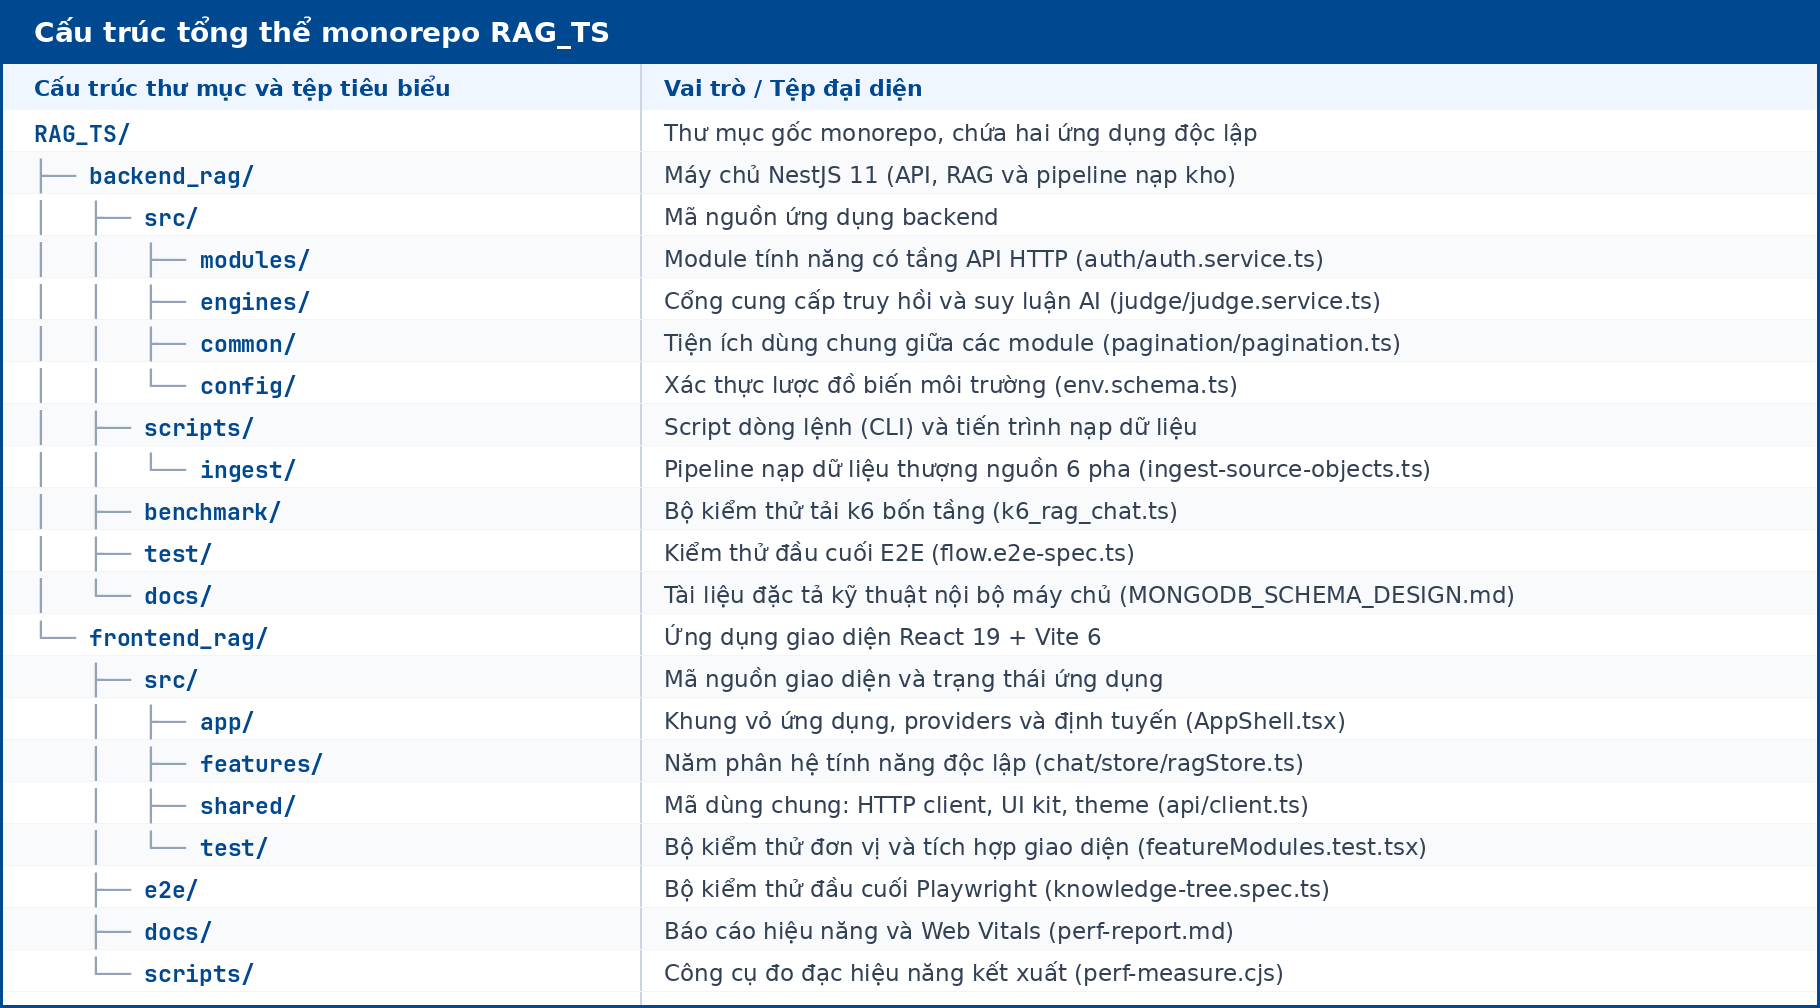
\includegraphics[width=0.95\textwidth]{assets/diagrams/tree-monorepo.png}
\caption{Cây thư mục của kho mã nguồn tới độ sâu ba cấp, kèm tệp đặc trưng tiêu biểu và trách nhiệm của từng thư mục}
\label{fig:cay-thu-muc-monorepo}
\end{figure}

Bên cạnh khối mã nguồn thực thi ở Hình~\ref{fig:cay-thu-muc-monorepo}, thư mục \texttt{docs/} chứa các đặc tả liên chương và \texttt{agents/} chứa quy chuẩn kỹ thuật biên soạn; việc tách biệt giúp cây mã nguồn chính chỉ tập trung vào ba khối được biên dịch, kiểm thử và đóng gói.

Bên trong \texttt{backend\_rag/src}, mã nguồn được tổ chức thành bốn tầng theo ranh giới trách nhiệm (Hình~\ref{fig:cay-thu-muc-backend}): tầng \texttt{modules/} chứa các phân hệ nghiệp vụ HTTP (\texttt{controller}, \texttt{service}, \texttt{DTO}, \texttt{schema} Mongoose); tầng \texttt{engines/} chứa các thành phần truy hồi và suy luận đứng sau cổng giao diện \texttt{Symbol}; tầng \texttt{common/} chứa bộ lọc lỗi, phân trang theo \texttt{cursor}, giới hạn tần suất và ngữ cảnh nhật ký; tầng \texttt{config/} chịu trách nhiệm xác thực biến môi trường. Ở phía giao diện, \texttt{frontend\_rag/src} áp dụng kiến trúc chia theo tính năng (\textit{vertical slice}) (Hình~\ref{fig:cay-thu-muc-frontend}).

\begin{figure}[htbp]
\centering
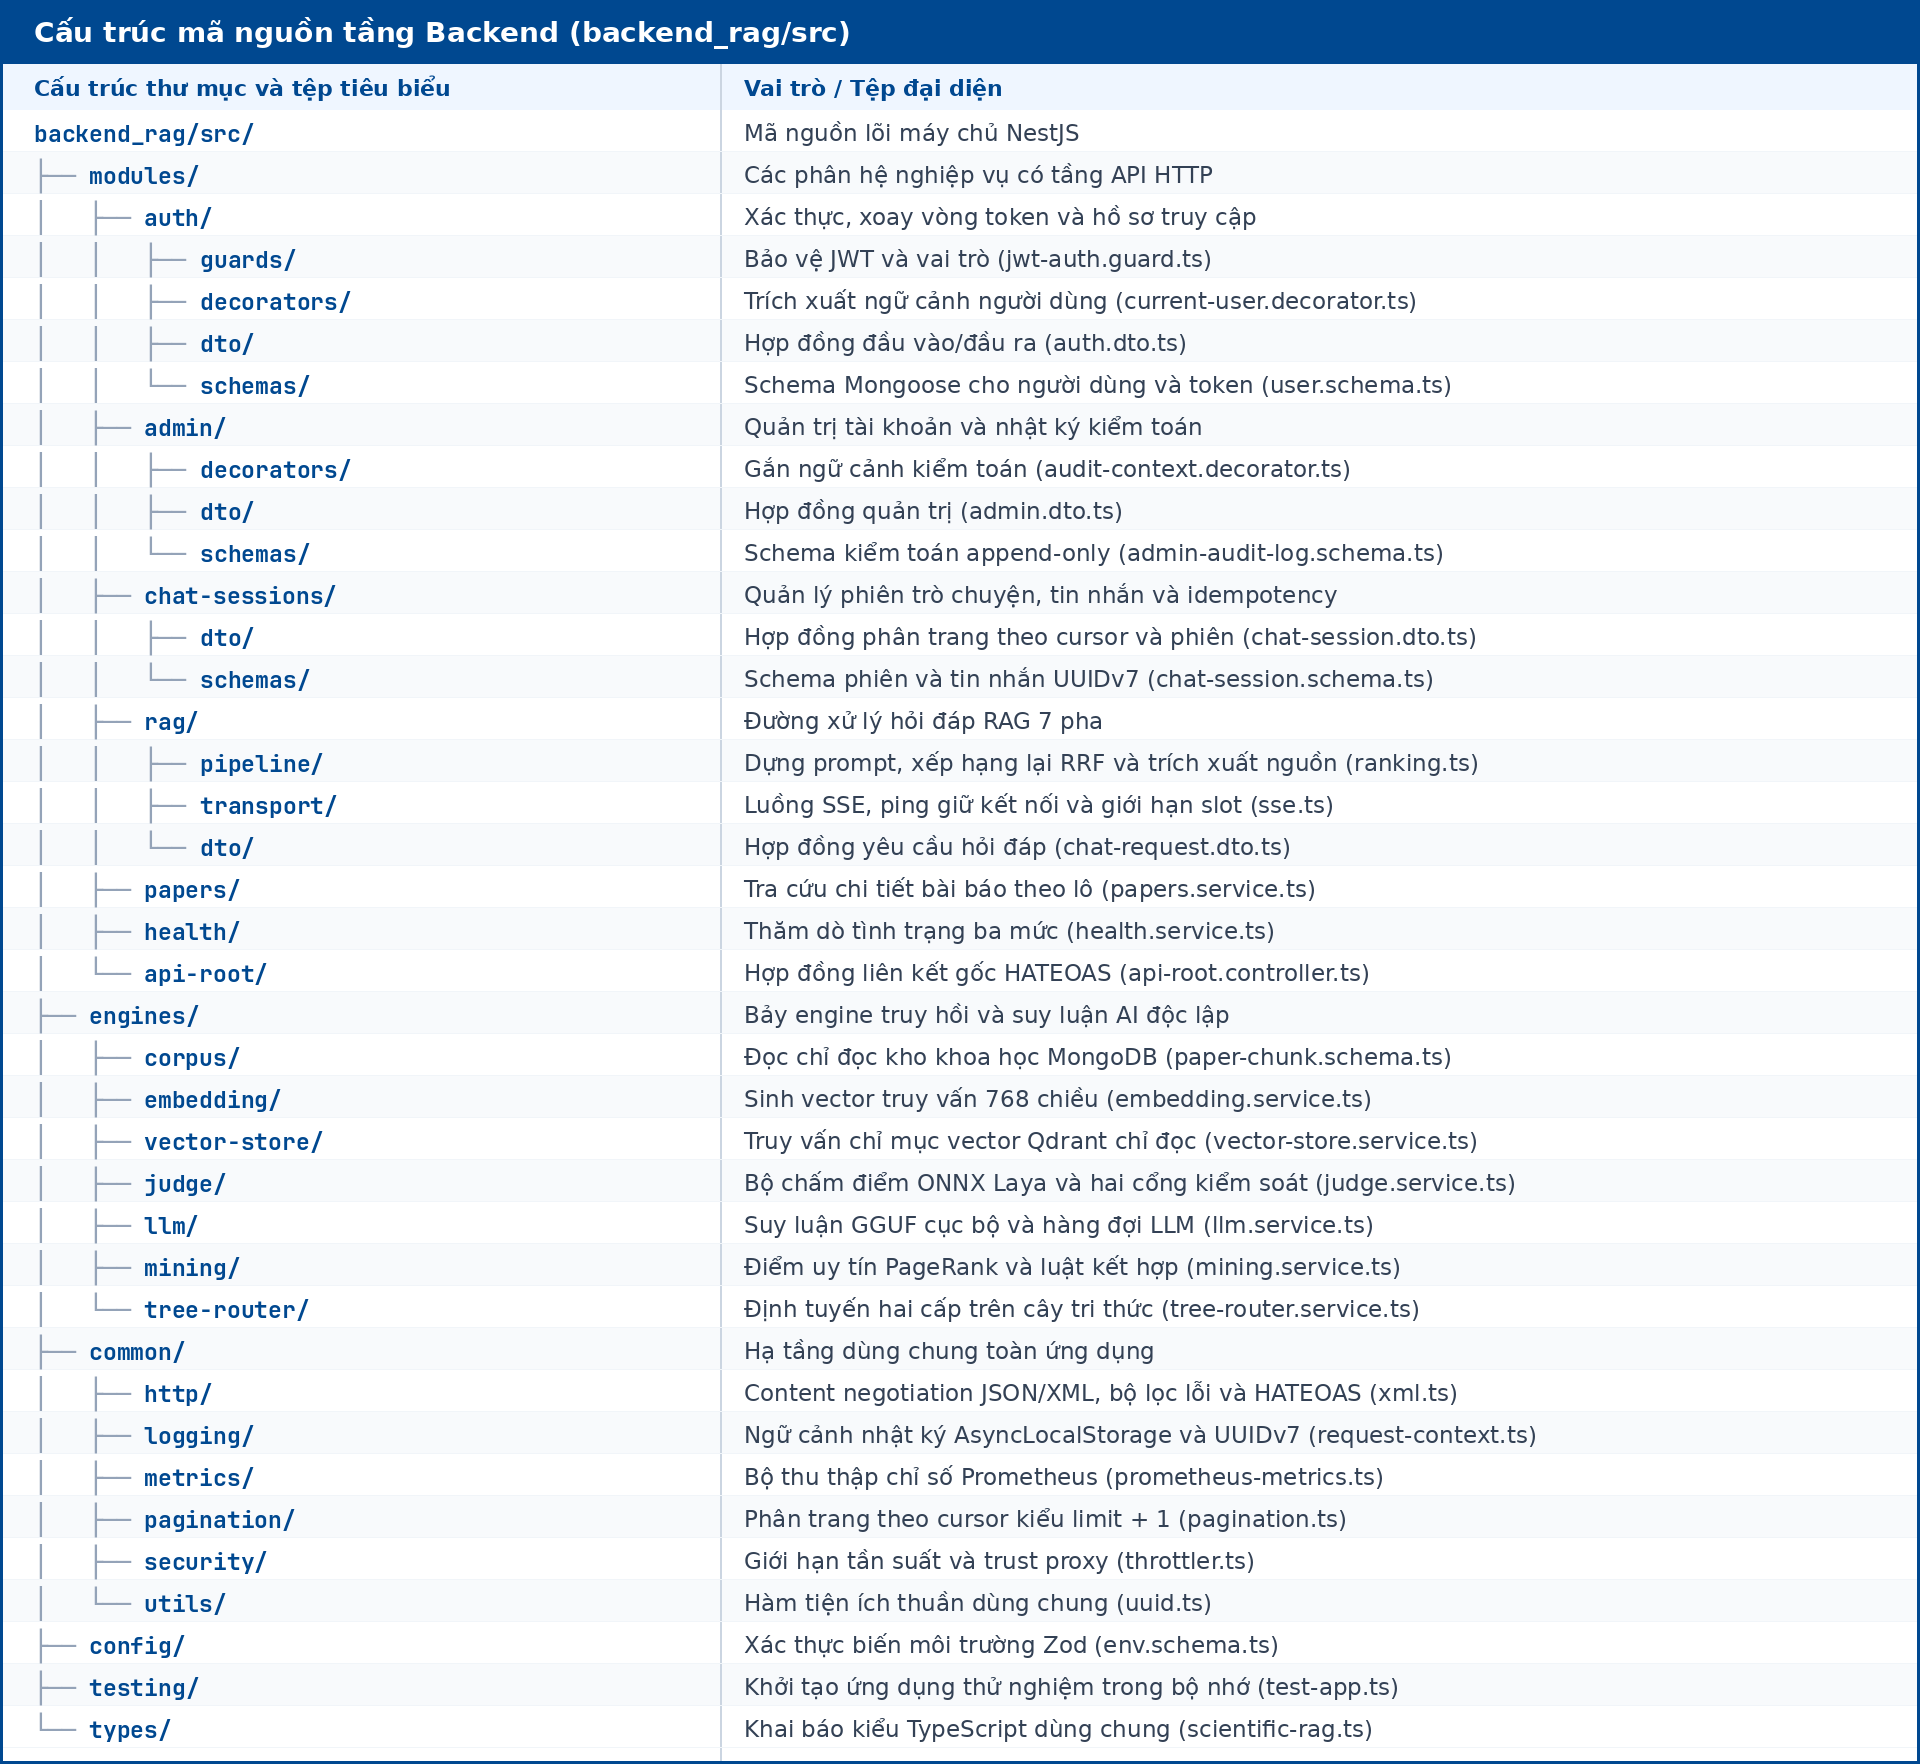
\includegraphics[width=0.95\textwidth,height=0.80\textheight,keepaspectratio]{assets/diagrams/tree-backend.png}
\caption{Cây thư mục tầng mã nguồn của máy chủ, theo ranh giới giữa tầng module, tầng engine và tầng mã dùng chung}
\label{fig:cay-thu-muc-backend}
\end{figure}

\begin{figure}[htbp]
\centering
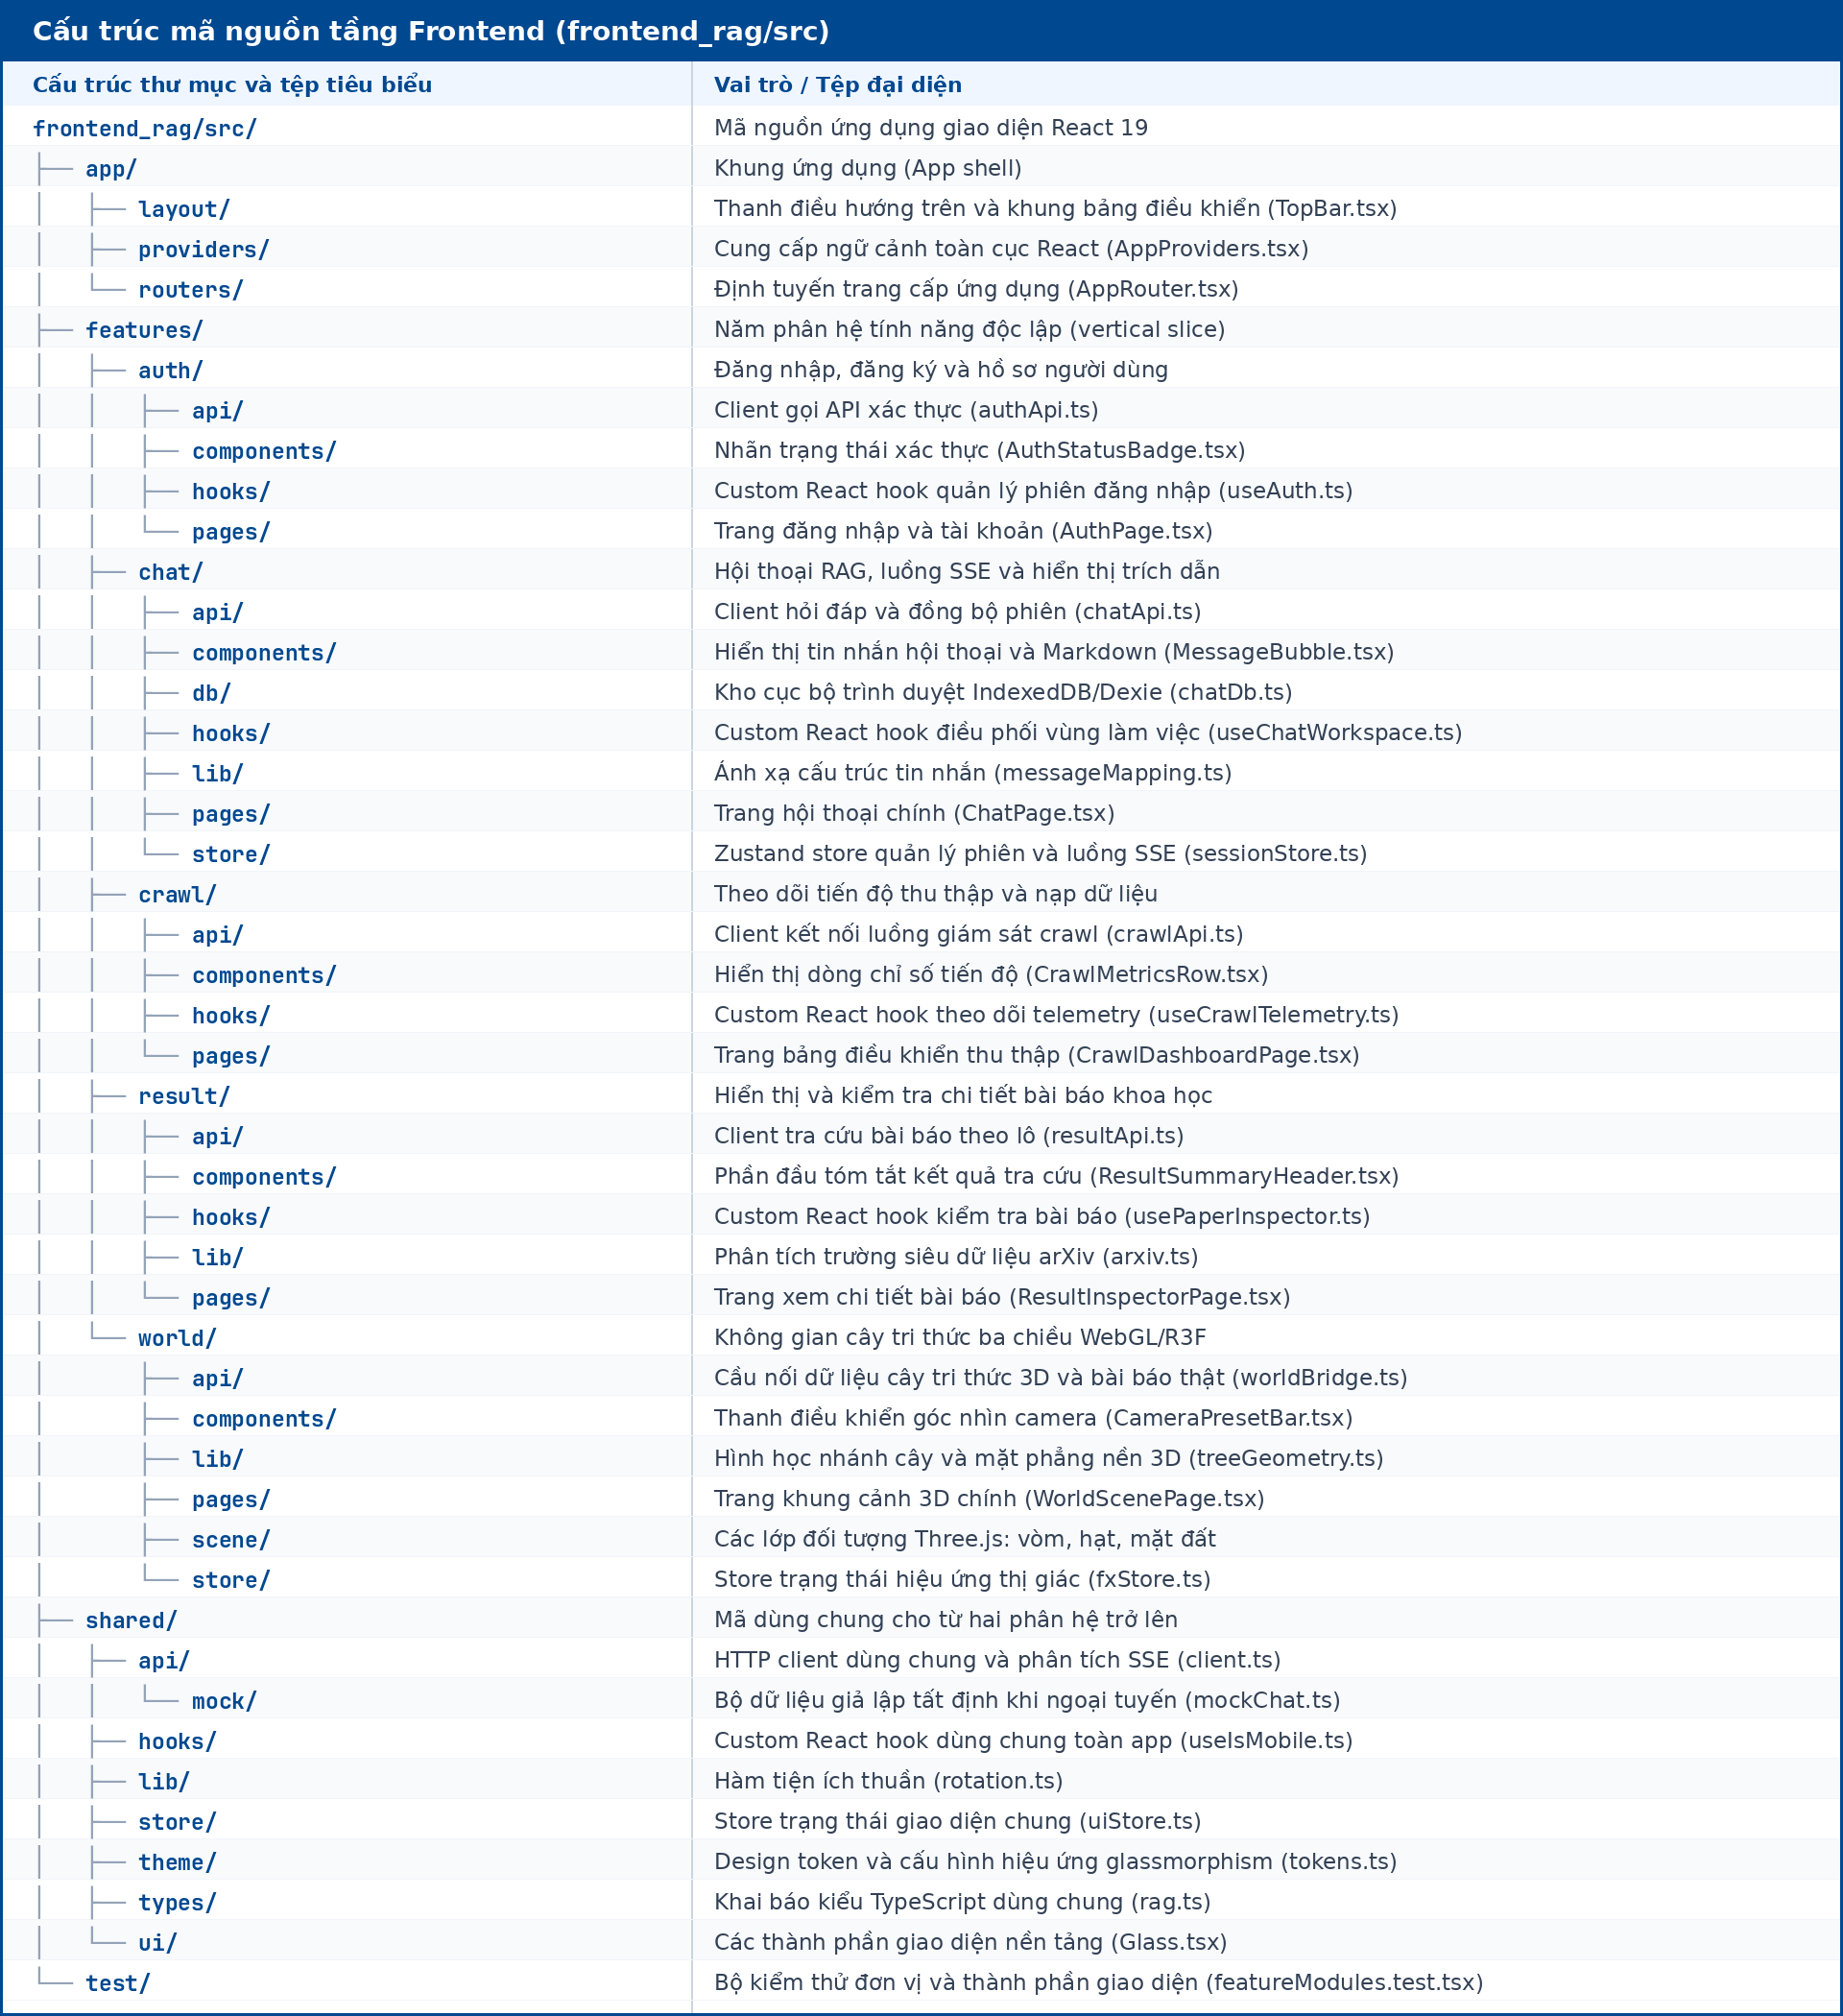
\includegraphics[width=0.95\textwidth,height=0.82\textheight,keepaspectratio]{assets/diagrams/tree-frontend.png}
\caption{Cây thư mục tầng mã nguồn của giao diện, theo kiến trúc vertical slice với năm tính năng độc lập}
\label{fig:cay-thu-muc-frontend}
\end{figure}

Nguyên tắc phân tách cổng và bộ chuyển đổi (\texttt{Ports and Adapters}) được hiện thực bằng cặp \texttt{interface} và định danh \texttt{Symbol} cho các engine cốt lõi. Nhờ cơ chế Dependency Injection (\texttt{DI}) qua \texttt{Symbol}, tầng \texttt{modules/} hoàn toàn không phụ thuộc trực tiếp vào thư viện hạ tầng và có thể thay thế mọi engine bằng bản \texttt{mock} khi chạy kiểm thử đơn vị:

\begin{tsbox}{Định nghĩa cổng giao diện nhúng bằng Symbol trong embedding.service.ts}
/** What the RAG pipeline needs from an embedder; mocked in tests. */
export interface EmbeddingPort {
  embedQuery(q: string): Promise<number[]>;
  isReady(): boolean;
}

export const EMBEDDING_PORT = Symbol('EMBEDDING_PORT');
\end{tsbox}

Hệ thống định nghĩa sáu cổng giao diện \texttt{Symbol} gồm \texttt{EMBEDDING\_\allowbreak{}PORT}, \texttt{VECTOR\_\allowbreak{}STORE\_\allowbreak{}PORT}, \texttt{LLM\_\allowbreak{}PORT}, \texttt{JUDGE\_\allowbreak{}PORT}, \texttt{CORPUS\_\allowbreak{}PORT} và \texttt{SESSION\_\allowbreak{}STORE}. Trong đó, cổng \texttt{SESSION\_\allowbreak{}STORE} nằm ở chiều ngược lại để phân hệ \texttt{rag} có thể lưu lượt hỏi đáp qua dịch vụ của \texttt{chat-\allowbreak{}sessions} mà không chứa bất kỳ truy vấn Mongoose nào bên trong pipeline AI. Hình~\ref{fig:ranh-gioi-ba-tang-be} minh hoạ ranh giới ba tầng của máy chủ thông qua các cổng giao diện này.

\begin{figure}[htbp]
\centering
\resizebox{\textwidth}{!}{%
\begin{tikzpicture}[
    node distance=0.35cm and 2.1cm,
    mnode/.style={ragbox, minimum width=3.2cm, minimum height=0.78cm, font=\footnotesize\sffamily},
    pnode/.style={ragbox, minimum width=4.1cm, minimum height=0.78cm, fill=primaryBlue!14, font=\footnotesize\ttfamily},
    enode/.style={ragbox, minimum width=3.4cm, minimum height=0.78cm, fill=primaryBlue!18, font=\footnotesize\sffamily}
]
    % Column 2: Ports (6 items)
    \node[pnode] (p1) {LLM\_PORT};
    \node[pnode, below=of p1] (p2) {VECTOR\_STORE\_PORT};
    \node[pnode, below=of p2] (p3) {EMBEDDING\_PORT};
    \node[pnode, below=of p3] (p4) {JUDGE\_PORT};
    \node[pnode, below=of p4] (p5) {CORPUS\_PORT};
    \node[pnode, below=of p5] (p6) {SESSION\_STORE};

    % Column 1: Modules (5 items aligned cleanly)
    \node[mnode, left=of p1] (rag) {\texttt{rag}};
    \node[mnode, left=of p2] (pap) {\texttt{papers}};
    \node[mnode, left=of p4] (aut) {\texttt{auth}};
    \node[mnode, left=of p5] (adm) {\texttt{admin}};
    \node[mnode, left=of p6] (chs) {\texttt{chat-sessions}};

    % Column 3: Engines (6 items)
    \node[enode, right=of p1] (e1) {\texttt{llm}};
    \node[enode, right=of p2] (e2) {\texttt{vector-store}};
    \node[enode, right=of p3] (e3) {\texttt{embedding}};
    \node[enode, right=of p4] (e4) {\texttt{judge}};
    \node[enode, right=of p5] (e5) {\texttt{corpus}};
    \node[enode, right=of p6] (e6) {\texttt{chat-sessions}};

    \begin{scope}[on background layer]
        \node[raggroup, fit=(rag)(chs), label={[font=\small\bfseries, text=primaryBlue, yshift=3pt]above:Tầng module (HTTP)}] {};
        \node[raggroup, fit=(p1)(p6), label={[font=\small\bfseries, text=primaryBlue, yshift=3pt]above:Cổng giao diện (Symbol)}] {};
        \node[raggroup, fit=(e1)(e6), label={[font=\small\bfseries, text=primaryBlue, yshift=3pt]above:Tầng engine (Hiện thực)}] {};
    \end{scope}

    % Connections
    \foreach \i in {1,...,6} {
        \draw[ragarrow] (rag.east) -- (p\i.west);
        \draw[ragarrow] (p\i.east) -- (e\i.west);
    }
    \draw[ragdashed] (pap.east) -- (p2.west);
    \draw[ragdashed] (pap.east) -- (p5.west);
    \draw[ragdashed] (chs.east) -- (p6.west);
\end{tikzpicture}%
}
\caption{Ranh giới ba tầng của máy chủ: phân hệ nghiệp vụ tiêu thụ engine qua cổng \texttt{Symbol}, không phụ thuộc trực tiếp vào hiện thực}
\label{fig:ranh-gioi-ba-tang-be}
\end{figure}

Về quản lý phụ thuộc phía máy chủ, cả \texttt{package.json} và tệp \texttt{lockfile} (\texttt{package-\allowbreak{}lock.\allowbreak{}json}) đều được theo dõi trong Git nhằm bảo đảm tính tái lập môi trường cho các phép đo hiệu năng tại Chương~\ref{chap:kiem-thu-danh-gia}. Bảng~\ref{tab:phu-thuoc-backend} tổng hợp 14~nhóm thư viện phụ thuộc chính của phân hệ backend.

\begingroup\footnotesize
\setlength{\tabcolsep}{4pt}
\begin{longtable}{
  @{}>{\raggedright\arraybackslash}p{2.7cm}
  >{\raggedright\arraybackslash}p{5.5cm}
  >{\raggedright\arraybackslash}p{7.0cm}@{}
}
\caption{Các phụ thuộc trực tiếp của máy chủ theo nhóm chức năng}
\label{tab:phu-thuoc-backend} \\
\toprule
\textbf{Nhóm} & \textbf{Phụ thuộc chính} & \textbf{Lý do lựa chọn} \\
\midrule
\endfirsthead
\caption[]{Các phụ thuộc trực tiếp của máy chủ theo nhóm chức năng (tiếp theo)} \\
\toprule
\textbf{Nhóm} & \textbf{Phụ thuộc chính} & \textbf{Lý do lựa chọn} \\
\midrule
\endhead
\midrule
\multicolumn{3}{r}{\textit{Xem tiếp ở trang sau}} \\
\endfoot
\bottomrule
\endlastfoot
\texttt{Framework} & \texttt{@nestjs/\allowbreak{}core}, \texttt{@nestjs/\allowbreak{}common}, \texttt{@nestjs/\allowbreak{}platform-\allowbreak{}express}~11; \texttt{reflect-\allowbreak{}metadata}, \texttt{rxjs} & Cung cấp cơ chế \texttt{DI}, module hoá và pipeline xử lý request chuẩn hoá \\
Kiểm tra dữ liệu & \texttt{class-\allowbreak{}validator}, \texttt{class-\allowbreak{}transformer} & Kiểm tra lược đồ \texttt{DTO} ngay tại biên HTTP trước khi vào tầng nghiệp vụ \\
Cấu hình & \texttt{zod}~4, \texttt{dotenv} & Xác thực biến môi trường kèm suy luận kiểu tĩnh và báo lỗi gom nhóm \\
Cơ sở dữ liệu & \texttt{mongoose}~8, \texttt{@nestjs/\allowbreak{}mongoose}~11 & Khai báo schema, chỉ mục tự động và truy vấn cơ sở dữ liệu ứng dụng \\
Chỉ mục vector & \texttt{@qdrant/\allowbreak{}js-\allowbreak{}client-\allowbreak{}rest} & Giao tiếp chỉ đọc với chỉ mục Qdrant qua bộ lọc có cấu trúc \\
Mô hình ngôn ngữ & \texttt{node-\allowbreak{}llama-\allowbreak{}cpp} & Suy luận GGUF cục bộ với tăng tốc CUDA và Metal, không gọi API ngoài \\
Mô hình nhúng & \texttt{@huggingface/\allowbreak{}transformers} & Thực thi mô hình nhúng ONNX cục bộ trong tiến trình Node.js \\
Bảo mật & \texttt{argon2}, \texttt{@nestjs/\allowbreak{}jwt}, \texttt{helmet} & Băm mật khẩu Argon2id, ký/xác minh JWT và thiết lập header bảo mật HTTP \\
Giới hạn tần suất (\texttt{rate limiting}) & \texttt{@nestjs/\allowbreak{}throttler} & Giới hạn tần suất theo địa chỉ IP kết hợp bộ đếm toàn cục và \texttt{decorator} theo route \\
Ghi nhật ký & \texttt{nestjs-\allowbreak{}pino}, \texttt{pino}, \texttt{pino-\allowbreak{}http} & Xuất nhật ký JSON một dòng gắn mã định danh yêu cầu \\
Đệm bộ nhớ & \texttt{lru-\allowbreak{}cache} & Bộ nhớ đệm trong tiến trình có giới hạn kích thước và \texttt{TTL} \\
Định dạng trao đổi & \texttt{fast-\allowbreak{}xml-\allowbreak{}parser} & \texttt{Content negotiation} cho XML và chặn khai báo \texttt{DOCTYPE}/\texttt{ENTITY} phòng chống \texttt{XXE} \\
Đặc tả API & \texttt{@nestjs/\allowbreak{}swagger}, \texttt{swagger-\allowbreak{}ui-\allowbreak{}express} & Sinh tài liệu OpenAPI~3.0 tự động ngoài môi trường production \\
Kiểm thử & \texttt{jest}~30, \texttt{ts-\allowbreak{}jest}, \texttt{supertest}, \texttt{mongodb-\allowbreak{}memory-\allowbreak{}server} & Kiểm thử đơn vị và tích hợp với cụm MongoDB chạy trong bộ nhớ \\
\end{longtable}
\endgroup

Về cấu hình TypeScript (\texttt{strict: true}), hai ứng dụng áp dụng hai điều chỉnh có chủ đích: phía backend trong \texttt{backend\_\allowbreak{}rag/\allowbreak{}tsconfig.\allowbreak{}json} tắt tuỳ chọn \texttt{strictProperty\allowbreak{}Initialization} (\texttt{false}) vì các lược đồ Mongoose gán thuộc tính qua decorator thay vì trong \texttt{constructor}; trong khi phía frontend tắt \texttt{noUnused\allowbreak{}Locals} và \texttt{noUnused\allowbreak{}Parameters} để tương thích với các thành phần React viết theo kiểu khai báo \texttt{callback}. Hai phía cũng dùng \texttt{moduleResolution} phù hợp với công cụ đóng gói: \texttt{commonjs} cho NestJS và \texttt{bundler} cho Vite.

\begin{minted}[fontsize=\footnotesize,breaklines,breakanywhere]{json}
{
  "compilerOptions": {
    "types": ["node", "jest"],
    "module": "commonjs",
    "esModuleInterop": true,
    "declaration": true,
    "removeComments": true,
    "emitDecoratorMetadata": true,
    "experimentalDecorators": true,
    "allowSyntheticDefaultImports": true,
    "resolveJsonModule": true,
    "target": "ES2023",
    "sourceMap": true,
    "outDir": "./dist",
    "baseUrl": "./",
    "incremental": true,
    "skipLibCheck": true,
    "strict": true,
    "strictPropertyInitialization": false,
    "forceConsistentCasingInFileNames": true,
    "noFallthroughCasesInSwitch": true,
    "noImplicitAny": true
  }
}
\end{minted}

% ==============================================================================
\section{Triển khai Backend}
\label{sec:trien-khai-backend}

Phân hệ backend áp dụng kiến trúc \textit{modular monolith} trên NestJS~11 gồm 34~\texttt{endpoint} dưới tiền tố \texttt{/api/v1}, cấu thành từ bảy module tính năng và bảy module engine.

\subsection{Xây dựng cấu trúc Backend và các module nghiệp vụ}
\label{subsec:backend-modules}

Module gốc \texttt{AppModule} làm điểm lắp ráp duy nhất cho hai kết nối Mongoose độc lập, bộ giới hạn tần suất toàn cục và danh sách các phân hệ nghiệp vụ (Bảng~\ref{tab:app-module-blocks}).

\begin{table}[htbp]
\centering
\caption{Các khối khai báo trong module gốc của máy chủ}
\label{tab:app-module-blocks}
\footnotesize
\setlength{\tabcolsep}{4pt}
\begin{tabularx}{\textwidth}{
  >{\raggedright\arraybackslash}p{3.4cm}
  >{\raggedright\arraybackslash}p{4.8cm}
  >{\raggedright\arraybackslash}X
}
\toprule
\textbf{Khối khai báo} & \textbf{Cấu hình chính} & \textbf{Ý nghĩa thiết kế} \\
\midrule
Kết nối Mongoose mặc định & \texttt{MONGO\_\allowbreak{}URI}, \texttt{serverSelection\allowbreak{}TimeoutMS:\allowbreak{} 5.000}, \texttt{maxPoolSize:\allowbreak{} 120}, \texttt{minPoolSize:\allowbreak{} 20}, \texttt{maxIdleTimeMS:\allowbreak{} 60.000} & Kết nối tới \texttt{rag\_ts}; duy trì \texttt{connection pool} lớn nhằm bù chi phí \texttt{round-trip} 15--25~ms qua \texttt{tunnel} \\
\midrule
Kết nối Mongoose \texttt{corpus} & \texttt{dbName} từ \texttt{MONGO\_\allowbreak{}CORPUS\_\allowbreak{}DB}, tên kết nối \texttt{corpus} & Tách biệt kết nối tới kho khoa học để đợt nạp hàng trăm nghìn tài liệu không làm nhiễu \texttt{working set} ứng dụng \\
\midrule
\texttt{ThrottlerModule.\allowbreak{}forRoot} & Một bộ giới hạn nền tên \texttt{default} (120~lượt/phút) & Các route nhạy cảm thu hẹp hạn mức riêng bằng \texttt{@RateLimit(...)}, tránh xung đột nhiều bộ giới hạn chồng chéo \\
\midrule
\texttt{APP\_GUARD} toàn ứng dụng & Đăng ký \texttt{ThrottlerGuard} ở cấp gốc & Mọi route mới bổ sung tự động kế thừa bảo vệ giới hạn tần suất mặc định \\
\midrule
\texttt{ApiRootController} & \texttt{GET /api/v1} & Điểm khởi đầu \texttt{HATEOAS} trả về liên kết tới các nhóm tài nguyên cấp cao \\
\bottomrule
\end{tabularx}
\end{table}

Đoạn mã lắp ráp hai kết nối Mongoose trong \texttt{backend\_\allowbreak{}rag/\allowbreak{}src/\allowbreak{}app.\allowbreak{}module.\allowbreak{}ts} cho thấy cách tách rời kết nối ứng dụng và kết nối kho khoa học ngay từ tầng khởi tạo:

\begin{tsbox}{Khai báo hai kết nối Mongoose tách biệt trong app.module.ts}
MongooseModule.forRootAsync({
  inject: [AppConfigService],
  useFactory: (config: AppConfigService) => ({
    uri: config.get('MONGO_URI'),
    serverSelectionTimeoutMS: 5000,
    maxPoolSize: 120,
    minPoolSize: 20,
    maxIdleTimeMS: 60_000,
  }),
}),
MongooseModule.forRootAsync({
  inject: [AppConfigService],
  useFactory: (config: AppConfigService) => ({
    uri: config.get('MONGO_CORPUS_URI') ?? config.get('MONGO_URI'),
    dbName: config.get('MONGO_CORPUS_DB'),
    serverSelectionTimeoutMS: 5000,
  }),
  connectionName: CORPUS_CONNECTION,
}),
\end{tsbox}

Mỗi module tính năng tuân theo bố cục bốn lớp thống nhất: \texttt{controller} (tầng API HTTP), \texttt{service} (logic nghiệp vụ), \texttt{dto/} (hợp đồng đầu vào/đầu ra) và \texttt{schemas/} (lược đồ Mongoose). Bảng~\ref{tab:bay-module-tinh-nang} và Bảng~\ref{tab:bay-module-engine} phân biệt ranh giới giữa bảy module nghiệp vụ và bảy module engine.

\begin{table}[htbp]
\centering
\caption{Bảy module tính năng, tầng API HTTP và quyền sở hữu dữ liệu}
\label{tab:bay-module-tinh-nang}
\footnotesize
\setlength{\tabcolsep}{4pt}
\begin{tabularx}{\textwidth}{
  >{\raggedright\arraybackslash}p{2.3cm}
  >{\raggedright\arraybackslash}p{4.4cm}
  >{\raggedright\arraybackslash}p{4.0cm}
  >{\raggedright\arraybackslash}X
}
\toprule
\textbf{Module} & \textbf{Đường dẫn chính} & \textbf{Collection sở hữu} & \textbf{Cơ chế bảo vệ} \\
\midrule
\texttt{auth} & \texttt{POST /auth/tokens}, \texttt{/auth/\allowbreak{}token-\allowbreak{}rotations}, \texttt{/auth/\allowbreak{}token-\allowbreak{}revocations} & \texttt{users}, \texttt{refresh\_\allowbreak{}tokens}, \texttt{login\_\allowbreak{}attempts} & \texttt{JwtAuthGuard} trên route thu hồi; \texttt{@RateLimit('login')} và \texttt{@RateLimit('refresh')} \\
\midrule
\texttt{admin} & \texttt{GET /admin/users}, \texttt{PUT /admin/\allowbreak{}users/\allowbreak{}:id/\allowbreak{}roles}, \texttt{/status}, \texttt{GET /admin/\allowbreak{}audit-\allowbreak{}logs} & \texttt{admin\_\allowbreak{}audit\_\allowbreak{}logs} (\texttt{append-\allowbreak{}only}) & Ba lớp: \texttt{JwtAuthGuard}, \texttt{RolesGuard}, kiểm tra lại ở tầng service \\
\midrule
\texttt{chat-\allowbreak{}sessions} & \texttt{GET /chat-\allowbreak{}sessions}, \texttt{/:id/\allowbreak{}messages}, \texttt{PATCH /:id}, \texttt{DELETE /:id} & \texttt{chat\_\allowbreak{}sessions}, \texttt{chat\_\allowbreak{}messages}, \texttt{chat\_\allowbreak{}requests} & Lọc \texttt{deleted\_\allowbreak{}at:\allowbreak{} null} và \texttt{user\_\allowbreak{}id}; trả \texttt{404} thay vì \texttt{403} \\
\midrule
\texttt{rag} & \texttt{POST /rag/chat}, \texttt{POST /rag/chat/stream} & Đọc Qdrant và kho khoa học; ghi phiên qua \texttt{SESSION\_\allowbreak{}STORE} & \texttt{OptionalJwtAuthGuard}; hạn mức 20~lượt/phút (đã đăng nhập), 10~lượt (khách) \\
\midrule
\texttt{papers} & \texttt{GET /papers}, \texttt{GET /papers/\allowbreak{}:paper\_\allowbreak{}id} & Không sở hữu \texttt{collection}; đọc kho khoa học và Qdrant & Chỉ đọc; trả \texttt{404} khi không tìm thấy \\
\midrule
\texttt{health} & \texttt{GET /health}, \texttt{/health/live}, \texttt{/health/ready} & Không có & Công khai; tác vụ kiểm tra nền (\texttt{background health probe}) mỗi 10~giây \\
\midrule
\texttt{api-root} & \texttt{GET /api/v1} & Không có & Công khai \\
\bottomrule
\end{tabularx}
\end{table}

Trong số bảy module engine, năm module (\texttt{embedding}, \texttt{vector-store}, \texttt{llm}, \texttt{judge}, \texttt{corpus}) đứng sau các cổng \texttt{Symbol} để có thể thay thế độc lập bằng bản \texttt{mock}, còn hai module (\texttt{mining}, \texttt{tree-router}) được \texttt{inject} trực tiếp theo đặc thù nạp dữ liệu tĩnh một lần (Bảng~\ref{tab:bay-module-engine}).

\begin{table}[htbp]
\centering
\caption{Bảy module engine, cổng giao diện và trách nhiệm hiện thực}
\label{tab:bay-module-engine}
\small
\begin{tabularx}{\textwidth}{
  >{\raggedright\arraybackslash}p{2.7cm}
  >{\raggedright\arraybackslash}p{4.1cm}
  >{\raggedright\arraybackslash}X
}
\toprule
\textbf{Module engine} & \textbf{Cổng / Cách tiêu thụ} & \textbf{Trách nhiệm hiện thực} \\
\midrule
\texttt{embedding} & \texttt{EMBEDDING\_\allowbreak{}PORT} & Nhúng câu hỏi thành vector 768~chiều kèm tiền tố \texttt{search\_query: } \\
\midrule
\texttt{vector-store} & \texttt{VECTOR\_\allowbreak{}STORE\_\allowbreak{}PORT} & Truy vấn Qdrant chỉ đọc theo bộ lọc danh mục/nhánh và nạp nội dung đoạn \\
\midrule
\texttt{llm} & \texttt{LLM\_\allowbreak{}PORT} & Suy luận cục bộ qua \texttt{node-\allowbreak{}llama-\allowbreak{}cpp} với hàng đợi 1~slot chạy và 8~chỗ chờ \\
\midrule
\texttt{judge} & \texttt{JUDGE\_\allowbreak{}PORT} & Đánh giá độ liên quan, độ căn cứ và xếp hạng lại qua mô hình ONNX Laya \\
\midrule
\texttt{corpus} & \texttt{CORPUS\_\allowbreak{}PORT} & Nạp nội dung đoạn trên đường xử lý chính và đọc dữ liệu đồ thị/cây ở \texttt{cold path} \\
\midrule
\texttt{mining} & \texttt{Inject} trực tiếp & Nạp điểm uy tín PageRank và luật kết hợp FP-Growth từ kho khoa học hoặc tệp đĩa \\
\midrule
\texttt{tree-router} & \texttt{Inject} trực tiếp & Định tuyến hai cấp trên cây tri thức dựa trên tâm cụm cấp~1 và cấp~2 \\
\bottomrule
\end{tabularx}
\end{table}

Nhờ ranh giới cổng giao diện này, tệp lắp ráp \texttt{RagModule} chỉ nhập các module cung cấp dịch vụ mà tầng nghiệp vụ hỏi đáp không hề chứa bất kỳ câu lệnh truy vấn cơ sở dữ liệu hay lời gọi thư viện AI cấp thấp nào:

\begin{tsbox}{Lắp ráp phụ thuộc qua module và cổng giao diện trong rag.module.ts}
@Module({
  imports: [
    EmbeddingModule,
    JudgeModule,
    VectorStoreModule,
    MiningModule,
    TreeRouterModule,
    LlmModule,
    ChatSessionsModule,
  ],
  controllers: [RagController],
  providers: [RagService],
})
export class RagModule {}
\end{tsbox}

Đối với tầng dữ liệu hội thoại, ba \texttt{collection} (\texttt{chat\_\allowbreak{}sessions}, \texttt{chat\_\allowbreak{}messages}, \texttt{chat\_\allowbreak{}requests}) sử dụng chuỗi \texttt{UUIDv7} sinh ở tầng ứng dụng làm \texttt{\_id} thay cho \texttt{ObjectId} của MongoDB. Thứ tự tăng dần theo thời gian của \texttt{UUIDv7} giúp phân trang theo \texttt{cursor} (\textit{cursor pagination}) giữ vị trí ổn định, đồng thời ngăn nguy cơ dò tìm tuần tự phiên của người dùng khác:

\begin{tsbox}{Lược đồ ChatSession với khoá chính UUIDv7 và chỉ mục TTL trong chat-session.schema.ts}
export class ChatSession {
  @Prop({ type: String, default: () => uuidv7() })
  _id: string;

  @Prop({ type: Types.ObjectId, required: true })
  user_id: Types.ObjectId;

  @Prop({ required: true })
  title: string;

  @Prop({ default: 0 })
  message_count: number;

  @Prop({ type: Date, default: () => new Date() })
  last_message_at: Date;

  @Prop({ type: Date, default: null })
  deleted_at: Date | null;

  created_at: Date;
  updated_at: Date;
}

export type ChatSessionDocument = HydratedDocument<ChatSession>;
export const ChatSessionSchema = SchemaFactory.createForClass(ChatSession);
ChatSessionSchema.index({
  user_id: 1,
  deleted_at: 1,
  last_message_at: -1,
  _id: -1,
});
ChatSessionSchema.index(
  { deleted_at: 1 },
  { expireAfterSeconds: SESSION_TTL_SECONDS },
);
\end{tsbox}

Chỉ mục kép trên bốn trường \texttt{\{ user\_\allowbreak{}id, deleted\_\allowbreak{}at, last\_\allowbreak{}message\_\allowbreak{}at: -1, \_id: -1 \}} phục vụ truy vấn danh sách phiên đang hoạt động sắp theo tin nhắn gần nhất, trong khi chỉ mục \texttt{TTL} trên \texttt{deleted\_\allowbreak{}at} tự động xoá vĩnh viễn phiên đã xoá mềm sau 259.200~giây (3~ngày) mà không cần tác vụ nền thủ công.

\subsection{Triển khai API và xử lý Request/Response}
\label{subsec:trien-khai-api}

Toàn bộ pipeline xử lý yêu cầu HTTP được đóng gói trong hàm \texttt{configureApp(app)} tại \texttt{backend\_\allowbreak{}rag/\allowbreak{}src/\allowbreak{}app.\allowbreak{}setup.\allowbreak{}ts}, bảo đảm máy chủ thực thi thật và ứng dụng kiểm thử E2E sử dụng chung cùng một chuỗi 12~bước từ lúc nhận request tới khi trả phản hồi (Hình~\ref{fig:chuoi-12-buoc-request} và Bảng~\ref{tab:muoi-hai-buoc-request}).

\begin{figure}[htbp]
\centering
\resizebox{\textwidth}{!}{%
\begin{tikzpicture}[
    node distance=0.8cm and 0.9cm,
    snode/.style={ragbox, text width=3.6cm, minimum height=1.15cm, font=\footnotesize\sffamily}
]
    % Row 1: 1 -> 2 -> 3 -> 4
    \node[snode] (s1) {\textbf{1. Gán định danh}\\(\texttt{X-Request-Id})};
    \node[snode, right=of s1] (s2) {\textbf{2. Bảo mật biên}\\Header HTTP \& \texttt{trust proxy}};
    \node[snode, right=of s2] (s3) {\textbf{3. Đo chỉ số}\\Histogram Prometheus};
    \node[snode, right=of s3] (s4) {\textbf{4. Kiểm tra body}\\Định dạng \& phân tích XML};

    % Row 2 (right to left: 5 -> 6 -> 7 -> 8)
    \node[snode, below=of s4] (s5) {\textbf{5. Giới hạn tần suất}\\\texttt{ThrottlerGuard}};
    \node[snode, left=of s5] (s6) {\textbf{6. Xác thực \& Quyền}\\\texttt{JwtAuth} \& \texttt{RolesGuard}};
    \node[snode, left=of s6] (s7) {\textbf{7. Kiểm tra \texttt{DTO}}\\\texttt{ValidationPipe} chặt chẽ};
    \node[snode, left=of s7] (s8) {\textbf{8. Nghiệp vụ}\\Controller \& Service};

    % Row 3 (left to right: 9 -> 10 -> 11 -> 12)
    \node[snode, below=of s8] (s9) {\textbf{9. Liên kết HATEOAS}\\Gắn \texttt{\_links}};
    \node[snode, right=of s9] (s10) {\textbf{10. Content negotiation}\\JSON hoặc XML};
    \node[snode, right=of s10] (s11) {\textbf{11. Lọc ngoại lệ}\\Chuẩn hoá error body};
    \node[snode, right=of s11] (s12) {\textbf{12. Nhật ký \& Trả về}\\Pino JSON \& phản hồi};

    \draw[ragarrow] (s1) -- (s2);
    \draw[ragarrow] (s2) -- (s3);
    \draw[ragarrow] (s3) -- (s4);
    \draw[ragarrow] (s4) -- (s5);
    \draw[ragarrow] (s5) -- (s6);
    \draw[ragarrow] (s6) -- (s7);
    \draw[ragarrow] (s7) -- (s8);
    \draw[ragarrow] (s8) -- (s9);
    \draw[ragarrow] (s9) -- (s10);
    \draw[ragarrow] (s10) -- (s11);
    \draw[ragarrow] (s11) -- (s12);
\end{tikzpicture}%
}
\caption{Chuỗi mười hai bước xử lý yêu cầu của máy chủ NestJS}
\label{fig:chuoi-12-buoc-request}
\end{figure}

\begingroup\footnotesize
\setlength{\tabcolsep}{4pt}
\begin{longtable}{
  @{}>{\raggedleft\arraybackslash}p{0.9cm}
  >{\raggedright\arraybackslash}p{3.4cm}
  >{\raggedright\arraybackslash}p{4.6cm}
  >{\raggedright\arraybackslash}p{6.1cm}@{}
}
\caption{Mười hai bước xử lý yêu cầu và hiện thực tương ứng}
\label{tab:muoi-hai-buoc-request} \\
\toprule
\textbf{Bước} & \textbf{Trách nhiệm} & \textbf{Cơ chế hiện thực} & \textbf{Lý do thiết kế} \\
\midrule
\endfirsthead
\caption[]{Mười hai bước xử lý yêu cầu và hiện thực tương ứng (tiếp theo)} \\
\toprule
\textbf{Bước} & \textbf{Trách nhiệm} & \textbf{Cơ chế hiện thực} & \textbf{Lý do thiết kế} \\
\midrule
\endhead
\midrule
\multicolumn{4}{r}{\textit{Xem tiếp ở trang sau}} \\
\endfoot
\bottomrule
\endlastfoot
1 & Gán mã định danh yêu cầu & \texttt{requestIdMiddleware} & Gắn \texttt{UUIDv7} vào ngữ cảnh \texttt{AsyncLocalStorage}, header \texttt{X-Request-Id} và mọi \texttt{error body} \\
2 & Bảo mật và tin cậy proxy & \texttt{securityHeaders}, \texttt{trustProxySetting} & Đặt \texttt{trust proxy} trước mọi lớp đọc IP để bộ giới hạn tần suất không khoá nhầm người dùng sau proxy \\
3 & Chỉ số Prometheus & \texttt{Prometheus\allowbreak{}Metrics\allowbreak{}Registry.\allowbreak{}middleware} & Ghi nhận histogram độ trễ và mã trạng thái HTTP không thêm truy vấn phụ \\
4 & Kiểm tra loại nội dung và XML & \texttt{unsupportedBody}, \texttt{xmlBodyMiddleware} & Chặn khai báo \texttt{DOCTYPE}/\texttt{ENTITY} ngay khi nhận \texttt{payload} XML để phòng chống \texttt{XXE} \\
5 & Giới hạn tần suất & \texttt{ThrottlerGuard} toàn cục, \texttt{@RateLimit(...)} & Bảo vệ nền mặc định toàn API và thu hẹp riêng cho route nhạy cảm \\
6 & Xác thực và phân quyền & \texttt{JwtAuthGuard}, \texttt{OptionalJwtAuthGuard}, \texttt{RolesGuard} & Tách biệt xác thực danh tính và kiểm tra quyền hạn tại biên HTTP \\
7 & Kiểm tra \texttt{DTO} & \texttt{createValidationPipe} & Loại bỏ và từ chối thuộc tính lạ ngoài lược đồ trước khi vào service \\
8 & Xử lý nghiệp vụ & Controller và Service & Tầng nghiệp vụ tách khỏi HTTP, cho phép kiểm thử độc lập \\
9 & Liên kết \texttt{HATEOAS} & \texttt{LinksInterceptor} & Gắn \texttt{\_links} cho các endpoint có \texttt{@WithLinks(...)} \\
10 & \texttt{Content negotiation} & \texttt{ContentNegotiation\allowbreak{}Interceptor} & Chuyển đổi linh hoạt JSON hoặc XML dựa theo header \texttt{Accept} \\
11 & Chuẩn hoá \texttt{error body} & \texttt{HttpExceptionFilter} & Đảm bảo cấu trúc phản hồi lỗi 4~trường đồng nhất cho mọi định dạng trao đổi \\
12 & Nhật ký và phản hồi & \texttt{nestjs-pino} (\texttt{pino-http}) & Ghi nhật ký một dòng JSON có lọc bỏ trường nhạy cảm \\
\end{longtable}
\endgroup

Hai cấu hình thứ tự trong \texttt{backend\_\allowbreak{}rag/\allowbreak{}src/\allowbreak{}app.\allowbreak{}setup.\allowbreak{}ts} mang tính quyết định đối với an ninh mạng: cấu hình \texttt{trust proxy} phải được áp dụng trước mọi middleware đọc \texttt{req.ip}, và tham số \texttt{TRUST\_\allowbreak{}PROXY\_\allowbreak{}HOPS} phải được truyền tường minh theo hạ tầng thực tế thay vì suy đoán từ \texttt{NODE\_\allowbreak{}ENV}:

\begin{tsbox}{Thiết lập trust proxy trước các middleware đọc IP trong app.setup.ts}
const express = app.getHttpAdapter().getInstance() as Express;
express.set(
  'trust proxy',
  trustProxySetting(nodeEnv, config.get('TRUST_PROXY_HOPS')),
);
app.use(requestIdMiddleware);
app.use(securityHeaders(isProduction));
\end{tsbox}

Tại bước~7, bộ kiểm tra (\texttt{backend\_\allowbreak{}rag/\allowbreak{}src/\allowbreak{}common/\allowbreak{}http/\allowbreak{}validation.\allowbreak{}ts}) bật cả \texttt{whitelist: true} lẫn \texttt{forbidNonWhitelisted: true} để ném lỗi~\texttt{400} ngay khi client gửi trường không khai báo, ngăn chặn lỗ hổng \textit{mass assignment} (ghi đè trường ngoài lược đồ) như chèn trường \texttt{role}:

\begin{tsbox}{Cấu hình ValidationPipe nghiêm ngặt trong validation.ts}
export function createValidationPipe(): ValidationPipe {
  return new ValidationPipe({
    whitelist: true,
    forbidNonWhitelisted: true,
    transform: true,
    exceptionFactory: (errors) =>
      new BadRequestException(firstValidationMessage(errors)),
  });
}
\end{tsbox}

Tại bước~4 và bước~10, bộ phân tích XML tuỳ biến trong \texttt{backend\_\allowbreak{}rag/\allowbreak{}src/\allowbreak{}common/\allowbreak{}http/\allowbreak{}xml.\allowbreak{}ts} vô hiệu hoá thuộc tính thẻ, giữ nguyên kiểu chuỗi (\texttt{parseTagValue: false} tránh biến mật khẩu thuần số thành kiểu số) và chặn thẳng biểu thức \texttt{<!DOCTYPE} hoặc \texttt{<!ENTITY} trước khi phân tích cú pháp:

\begin{tsbox}{Phân tích XML an toàn và chặn XXE trong xml.ts}
const parser = new XMLParser({
  ignoreAttributes: true,
  // Tag values stay strings: a numeric password or title must not turn into a number.
  parseTagValue: false,
  isArray: (name) => ARRAY_FIELDS.has(name),
  tagValueProcessor: (name, value) =>
    BOOLEAN_FIELDS.has(name) && (value === 'true' || value === 'false')
      ? value === 'true'
      : value,
});
const builder = new XMLBuilder({ ignoreAttributes: true });

export function toXml(body: unknown): string {
  return `<?xml version="1.0" encoding="UTF-8"?>${builder.build({ response: body })}`;
}

/** Any well-formed document with one root element -> the object inside that root. */
export function parseXmlBody(xml: string): Record<string, unknown> {
  // No document type means no entity expansion and no external entities (XXE, billion laughs).
  if (/<!DOCTYPE|<!ENTITY/i.test(xml) || XMLValidator.validate(xml) !== true) {
    throw new BadRequestException('invalid xml');
  }
\end{tsbox}

Tại bước~11, mọi ngoại lệ HTTP đi qua \texttt{backend\_\allowbreak{}rag/\allowbreak{}src/\allowbreak{}common/\allowbreak{}http/\allowbreak{}http-\allowbreak{}exception.\allowbreak{}filter.\allowbreak{}ts} đều chuẩn hoá về cấu trúc \texttt{error body} bốn trường thống nhất gồm \texttt{statusCode}, \texttt{error}, \texttt{message} (mã lỗi chuẩn hoá như \texttt{session \allowbreak{}not \allowbreak{}found}, \texttt{llm \allowbreak{}timeout}) và \texttt{request\_\allowbreak{}id}:

\begin{tsbox}{Chuẩn hoá cấu trúc phản hồi lỗi bốn trường trong http-exception.filter.ts}
export interface ErrorBody {
  statusCode: number;
  error: string;
  message: string;
  request_id: string | null;
}

export function messageOf(exception: HttpException): string {
  const res = exception.getResponse();
  if (typeof res === 'string') return res;
  const m = (res as { message?: unknown }).message;
  if (Array.isArray(m)) return String(m[0] ?? exception.message);
  if (typeof m === 'string') return m;
  return exception.message;
}
\end{tsbox}

Cơ chế phân trang cho mọi danh sách dùng chung bộ lọc phân trang theo \texttt{cursor} tại \texttt{backend\_\allowbreak{}rag/\allowbreak{}src/\allowbreak{}common/\allowbreak{}pagination/\allowbreak{}pagination.\allowbreak{}ts}. Con trỏ \texttt{cursor} được ràng buộc chặt với khoá sắp xếp (\texttt{sort}); nếu người gọi tái sử dụng \texttt{cursor} cũ với thứ tự sắp xếp khác, hệ thống trả về \texttt{400 invalid cursor} thay vì âm thầm bỏ sót dữ liệu. Kỹ thuật truy vấn \texttt{limit + 1} bản ghi cho phép xác định \texttt{has\_more} chỉ bằng một lượt truy vấn duy nhất mà không cần chạy thêm truy vấn \texttt{countDocuments}:

\begin{tsbox}{Bộ lọc con trỏ ràng buộc thứ tự và kỹ thuật limit + 1 trong pagination.ts}
/**
 * Keyset condition for "rows after the cursor". The cursor is bound to its sort order: reusing it
 * with another `sort` -> 400 `invalid cursor`, instead of silently skipping or repeating rows.
 */
export function keysetFilter(
  raw: string,
  terms: SortTerm[],
  spec: ListSpec,
): MongoFilter {
  const c = decodeCursor(raw, isKeysetCursor);
  if (c.s !== sortKey(terms) || c.v.length !== terms.length) {
    throw new BadRequestException(INVALID_CURSOR);
  }
  let id: unknown;
  let values: unknown[];
  try {
    if (spec.idType === 'uuid' && !isUuid(c.id)) throw new Error('bad id');
    id = parseValue(spec.idType === 'uuid' ? 'string' : 'objectId', c.id);
    values = terms.map((t, i) =>
      parseValue(spec.sortable[t.field], String(c.v[i])),
    );
  } catch {
    throw new BadRequestException(INVALID_CURSOR);
  }
  const or: MongoFilter[] = [];
  const equal: MongoFilter = {};
  terms.forEach((t, i) => {
    const op = t.dir === 'asc' ? '$gt' : '$lt';
    or.push({ ...equal, [t.field]: { [op]: values[i] } });
    equal[t.field] = values[i];
  });
  const idOp = terms.at(-1)?.dir === 'asc' ? '$gt' : '$lt';
  or.push({ ...equal, _id: { [idOp]: id } });
  return { $or: or };
}

/** One `limit + 1` result set -> the page envelope every list endpoint returns. */
export function toCursorPage<R extends object, T>(
  rows: R[],
  limit: number,
  terms: SortTerm[],
  map: (row: R) => T,
): { items: T[]; next_cursor: string | null; has_more: boolean } {
  const hasMore = rows.length > limit;
  const page = rows.slice(0, limit);
  const last = page.at(-1) as
    | (Record<string, unknown> & { _id: unknown })
    | undefined;
  return {
    items: page.map(map),
    next_cursor:
      hasMore && last
        ? encodeCursor({
            s: sortKey(terms),
            v: terms.map((t) => {
              const v = last[t.field] ?? last.created_at;
              return v instanceof Date ? v.toISOString() : v;
            }),
            id: String(last._id),
          })
        : null,
    has_more: hasMore,
  };
}
\end{tsbox}

Tại bước~9, thành phần gắn liên kết \texttt{HATEOAS} (\texttt{backend\_\allowbreak{}rag/\allowbreak{}src/\allowbreak{}common/\allowbreak{}http/\allowbreak{}hateoas.\allowbreak{}ts}) cung cấp tập hành động chuyển tiếp cho từng tài nguyên:

\begin{tsbox}{Định nghĩa liên kết HATEOAS cho tài khoản và phiên trò chuyện trong hateoas.ts}
export const accountLinks = (): Links => ({
  self: get('/users/me'),
  update: act('PATCH', '/users/me'),
  password: act('PUT', '/users/me/password'),
  'chat-sessions': get('/chat-sessions'),
  'token-rotations': act('POST', '/auth/token-rotations'),
  'token-revocations': act('POST', '/auth/token-revocations'),
});

export const sessionLinks = (id: string): Links => ({
  self: get(`/chat-sessions/${id}`),
  messages: get(`/chat-sessions/${id}/messages`),
  rename: act('PATCH', `/chat-sessions/${id}`),
  delete: act('DELETE', `/chat-sessions/${id}`),
  chat: act('POST', '/rag/chat'),
});
\end{tsbox}

Trên nhóm endpoint hỏi đáp, \texttt{POST /rag/chat} trả về câu trả lời hoàn chỉnh trong một phản hồi HTTP, còn \texttt{POST /rag/chat/stream} phát tuần tự từng token theo chuẩn \texttt{SSE} thông qua \texttt{SseWriter} (\texttt{backend\_\allowbreak{}rag/\allowbreak{}src/\allowbreak{}modules/\allowbreak{}rag/\allowbreak{}transport/\allowbreak{}sse.\allowbreak{}ts}). Hai chi tiết thiết kế quan trọng gồm header \texttt{X-\allowbreak{}Accel-\allowbreak{}Buffering:\allowbreak{} no} (ngăn proxy trung gian gom gói làm đơ luồng token) và \texttt{listener} \texttt{prependListener(\allowbreak{}'close',\allowbreak{} ...)} chạy trước \texttt{pino-http} để kích hoạt \texttt{AbortController} giải phóng hàng đợi ngay khi người dùng đóng kết nối:

\begin{tsbox}{Truyền phát SSE và huỷ lượt sinh khi client đóng kết nối trong sse.ts}
/** Server-Sent Events over a raw Express response (POST, so `@Sse()` cannot be used). */
export class SseWriter {
  private ping: NodeJS.Timeout | null = null;

  constructor(private readonly res: Response) {}

  /** Sends the headers right away so proxies and the browser start reading. */
  open(): void {
    this.res.status(200);
    this.res.setHeader('Content-Type', 'text/event-stream; charset=utf-8');
    this.res.setHeader('Cache-Control', 'no-cache, no-transform');
    this.res.setHeader('Connection', 'keep-alive');
    this.res.setHeader('X-Accel-Buffering', 'no');
    this.res.socket?.setNoDelay(true);
    this.res.flushHeaders();
    this.write(': ok\n\n');
    this.ping = setInterval(() => this.write(': ping\n\n'), PING_INTERVAL_MS);
  }
}

/**
 * Aborts when the client goes away before the response is complete. The listener runs before
 * pino-http's own `close` listener, so the request line is logged as `abortedEvent`.
 */
export function abortOnClientClose(
  res: Response,
  abortedEvent: string,
): AbortController {
  const ctrl = new AbortController();
  res.prependListener('close', () => {
    if (res.writableFinished) return;
    const ctx = contextOf(res);
    if (ctx) ctx.event = abortedEvent;
    ctrl.abort();
  });
  return ctrl;
}
\end{tsbox}

\subsection{Triển khai Authentication và Authorization}
\label{subsec:trien-khai-auth}

Hệ thống xác thực và phân quyền được hiện thực dựa trên nguyên tắc mọi thay đổi về trạng thái tài khoản hoặc vai trò phải vô hiệu hoá tức thì token đang hoạt động, đồng thời chống dò tài khoản bằng thời gian phản hồi đồng nhất. Bảng~\ref{tab:thong-so-bao-mat-ch5} tổng hợp 11~thông số bảo mật đã hiện thực.

\begingroup\footnotesize
\setlength{\tabcolsep}{4pt}
\begin{longtable}{
  @{}>{\raggedright\arraybackslash}p{3.0cm}
  >{\raggedright\arraybackslash}p{2.7cm}
  >{\raggedright\arraybackslash}p{4.6cm}
  >{\raggedright\arraybackslash}p{4.7cm}@{}
}
\caption{Thông số bảo mật và cơ chế hiện thực tương ứng}
\label{tab:thong-so-bao-mat-ch5} \\
\toprule
\textbf{Thông số} & \textbf{Giá trị} & \textbf{Cơ chế hiện thực} & \textbf{Lý do thiết kế} \\
\midrule
\endfirsthead
\caption[]{Thông số bảo mật và cơ chế hiện thực tương ứng (tiếp theo)} \\
\toprule
\textbf{Thông số} & \textbf{Giá trị} & \textbf{Cơ chế hiện thực} & \textbf{Lý do thiết kế} \\
\midrule
\endhead
\midrule
\multicolumn{4}{r}{\textit{Xem tiếp ở trang sau}} \\
\endfoot
\bottomrule
\endlastfoot
Thuật toán băm mật khẩu & Argon2id & \texttt{memoryCost:\allowbreak{} 65.536}~KiB, \texttt{timeCost:\allowbreak{} 3}, \texttt{parallelism:\allowbreak{} 4} & Kháng tấn công phần cứng chuyên dụng GPU/ASIC và tấn công kênh bên \\
\texttt{thread pool} Node.js & 4 & Gán \texttt{UV\_\allowbreak{}THREADPOOL\_\allowbreak{}SIZE = 4} đầu tệp \texttt{src/main.ts} & Khớp mức song song của Argon2id, cô lập tác vụ mật mã khỏi endpoint nhẹ (Mục~\ref{subsec:tang-3-crypto}) \\
Giới hạn đăng nhập sai & 5~lần/chu kỳ & Đếm nhanh trong bộ nhớ đệm (\texttt{TTL} 15~phút) kèm ghi \texttt{login\_attempts} & Khoá tạm thời tức thời trong tiến trình đồng thời lưu dấu vết quản trị \\
Chống dò email & Mật khẩu giả & Luôn thực thi \texttt{argon2.verify} với chuỗi băm giả khi không tìm thấy email & Thời gian phản hồi đồng đều giữa email đã đăng ký và chưa đăng ký \\
Thời hạn access token & 15~phút & \texttt{ACCESS\_\allowbreak{}TTL\_\allowbreak{}SECONDS} & Rút ngắn cửa sổ rủi ro khi token truy cập bị rò rỉ \\
Thời hạn refresh token & 7~ngày & \texttt{REFRESH\_\allowbreak{}TTL\_\allowbreak{}SECONDS} & Cân bằng trải nghiệm phiên đăng nhập và giới hạn thời gian tồn tại \\
Xoay vòng refresh token & Dùng 1~lần theo họ token & Cập nhật nguyên tử điều kiện \texttt{revoked\_\allowbreak{}at:\allowbreak{} null}; tái sử dụng $\implies$ thu hồi cả họ & Phát hiện và vô hiệu hoá ngay cả họ token khi bị đánh cắp \\
Thu hồi token đang hoạt động & \texttt{token\_version} trong claim \texttt{ver} & Đối chiếu \texttt{user.token\_version} tại \texttt{JwtAuthGuard} & Thu hồi tức thời access token khi đổi vai trò hoặc khoá tài khoản \\
Bộ nhớ đệm trạng thái & LRU 5.000~mục, \texttt{TTL} 5~giây & \texttt{tokenVersionCache} dùng \texttt{TTL} cố định (\texttt{updateAgeOnGet:\allowbreak{} false}) & Giảm truy vấn MongoDB nhưng vẫn bảo đảm cận trên thời gian có hiệu lực khi thay đổi quyền \\
Chính sách mật khẩu & 10--200~ký tự & \texttt{validatePassword} chặn 200~mật khẩu yếu phổ biến và phần tên email & Ngăn mật khẩu dễ đoán mà không áp đặt quy tắc ký tự phức tạp gây khó nhớ \\
Tạo tài khoản quản trị & Qua CLI cục bộ & Lệnh \texttt{npm run create:admin} & Không tồn tại API tạo hay tự nâng quyền quản trị viên qua mạng \\
\end{longtable}
\endgroup

Trong dịch vụ xác thực (\texttt{backend\_\allowbreak{}rag/\allowbreak{}src/\allowbreak{}modules/\allowbreak{}auth/\allowbreak{}auth.\allowbreak{}service.\allowbreak{}ts}), ba thông số của Argon2id được cố định thành hằng số \texttt{ARGON2\_\allowbreak{}OPTIONS}, còn bộ nhớ đệm hồ sơ người dùng giới hạn ở 5.000~mục. Khi email chưa tồn tại, hàm \texttt{dummyHash()} tạo một chuỗi băm Argon2id giả theo đúng cấu hình trên để \texttt{argon2.verify} luôn tiêu tốn cùng thời gian tính toán:

\begin{tsbox}{Băm mật khẩu Argon2id và chống dò tài khoản trong auth.service.ts}
export const ARGON2_OPTIONS: argon2.HashOptions = {
  type: argon2.argon2id,
  memoryCost: 65536,
  timeCost: 3,
  parallelism: 4,
};

// Always run Argon2id against the dummy hash when the email is unknown so response time
// cannot be used to tell registered emails from unregistered ones.
const ok = await argon2.verify(
  user ? user.password_hash : await this.dummyHash(),
  dto.password,
);
if (!user || !ok) {
  this.attemptCountCache.set(key, attemptCount + 1);
  await this.attempts.create({ key });
  logEvent('LOGIN_FAILED', { email_hash: emailHash(email) });
  throw new UnauthorizedException('invalid credentials');
}
\end{tsbox}

Cơ chế xoay vòng refresh token trong \texttt{backend\_\allowbreak{}rag/\allowbreak{}src/\allowbreak{}modules/\allowbreak{}auth/\allowbreak{}token.\allowbreak{}service.\allowbreak{}ts} cố ý \textbf{không \texttt{idempotent} (\textit{non-idempotent})}: thao tác \texttt{findOneAndUpdate} với điều kiện \texttt{revoked\_\allowbreak{}at:\allowbreak{} null} chỉ cho phép đúng một yêu cầu đồng thời thắng cuộc. Mọi nỗ lực dùng lại token đã đánh dấu thu hồi lập tức gọi \texttt{revokeFamily} để huỷ toàn bộ họ token:

\begin{tsbox}{Xoay vòng refresh token theo cơ chế atomic và thu hồi họ token trong token.service.ts}
async consume(raw: string): Promise<ConsumeResult> {
  const hash = this.hashRefresh(raw);
  const now = new Date();
  const won = await this.refreshTokens
    .findOneAndUpdate(
      { token_hash: hash, revoked_at: null, expires_at: { $gt: now } },
      { $set: { revoked_at: now } },
    )
    .lean();
  if (won) {
    return {
      ok: true,
      userId: won.user_id.toString(),
      familyId: won.family_id,
    };
  }
  const rec = await this.refreshTokens.findOne({ token_hash: hash }).lean();
  if (!rec) return { ok: false, reason: 'invalid' };
  if (rec.expires_at.getTime() <= now.getTime())
    return { ok: false, reason: 'expired' };
  if (rec.revoked_at) {
    await this.revokeFamily(rec.family_id);
    return { ok: false, reason: 'reused' };
  }
  return { ok: false, reason: 'race' };
}
\end{tsbox}

Tại tầng kiểm tra access token, \texttt{JwtAuthGuard} trong \texttt{backend\_\allowbreak{}rag/\allowbreak{}src/\allowbreak{}modules/\allowbreak{}auth/\allowbreak{}guards/\allowbreak{}jwt-\allowbreak{}auth.\allowbreak{}guard.\allowbreak{}ts} truy vấn trạng thái người dùng trên mỗi lượt gọi (qua bộ nhớ đệm \texttt{TTL} cố định 5~giây) để kiểm tra cờ \texttt{is\_active} và đối chiếu \texttt{token\_version}:

\begin{tsbox}{Kiểm tra trạng thái tài khoản và token\_version trong jwt-auth.guard.ts}
async canActivate(ctx: ExecutionContext): Promise<boolean> {
  const req = ctx.switchToHttp().getRequest<Request>();
  const token = bearerToken(req);
  if (!token) throw new UnauthorizedException(UNAUTHORIZED);
  const claims = await this.tokens.verifyAccess(token);
  // Check account state on every request so a disabled account or stale token fails immediately.
  const user = await this.auth.getActiveUser(claims.id);
  if (!user || !user.is_active) throw new UnauthorizedException(UNAUTHORIZED);
  if ((user.token_version ?? 0) !== (claims.tokenVersion ?? 0)) {
    throw new UnauthorizedException(UNAUTHORIZED);
  }
  req.user = {
    id: user._id.toString(),
    roles: user.roles,
    email: user.email,
  };
  return true;
}
\end{tsbox}

Phân quyền quản trị áp dụng phòng thủ nhiều lớp (\textit{defense in depth}): ngoài \texttt{JwtAuth\allowbreak{}Guard} và \texttt{Roles\allowbreak{}Guard}, tầng dịch vụ luôn gọi kiểm tra lại \texttt{assertAdmin} tại \texttt{backend\_\allowbreak{}rag/\allowbreak{}src/\allowbreak{}modules/\allowbreak{}admin/\allowbreak{}assert-\allowbreak{}admin.\allowbreak{}ts}. Song song đó, dịch vụ \texttt{Admin\allowbreak{}Identity\allowbreak{}Service} trong \texttt{backend\_\allowbreak{}rag/\allowbreak{}src/\allowbreak{}modules/\allowbreak{}admin/\allowbreak{}admin-\allowbreak{}identity.\allowbreak{}service.\allowbreak{}ts} ngăn quản trị viên tự khoá chính mình hoặc xoá vai trò quản trị cuối cùng bằng mã \texttt{HTTP 409 Conflict}:

\begin{tsbox}{Phòng thủ nhiều lớp và ngăn quản trị viên tự khoá tài khoản trong mô đun admin}
export function assertAdmin(actor: AuthUser): void {
  if (!actor.roles.includes('admin')) {
    throw new ForbiddenException(ADMIN_ROLE_REQUIRED);
  }
}

/** An admin may not remove their own admin role or lock their own account. */
assertNotSelf(actor: AuthUser, targetId: string): void {
  if (actor.id === targetId) {
    throw new ConflictException(SELF_LOCKOUT_FORBIDDEN);
  }
}

async countActiveAdmins(): Promise<number> {
  return this.users.countDocuments({ roles: 'admin', is_active: true });
}

/** Keep at least one active admin at all times. */
async assertNotLastAdmin(target: LeanUser): Promise<void> {
  if (!target.roles.includes('admin')) return;
  if ((await this.countActiveAdmins()) <= 1) {
    throw new ConflictException(LAST_ADMIN_PROTECTED);
  }
}
\end{tsbox}

Mọi thao tác trên phân hệ quản trị đều được ghi vào \texttt{collection} bất biến \texttt{admin\_\allowbreak{}audit\_\allowbreak{}logs}; lớp \texttt{AdminAudit\allowbreak{}Service} chỉ cung cấp phương thức ghi bổ sung và liệt kê (\texttt{listAudit\allowbreak{}Logs}), tuyệt đối không cài đặt phương thức sửa hay xoá bản ghi.

Để bảo vệ tài nguyên máy chủ, \texttt{backend\_\allowbreak{}rag/\allowbreak{}src/\allowbreak{}common/\allowbreak{}security/\allowbreak{}throttler.\allowbreak{}ts} khai báo tập trung tám nhóm hạn mức theo chi phí xử lý, kết hợp giới hạn đồng thời theo người dùng và địa chỉ IP trong \texttt{backend\_\allowbreak{}rag/\allowbreak{}src/\allowbreak{}modules/\allowbreak{}rag/\allowbreak{}transport/\allowbreak{}client-\allowbreak{}slots.\allowbreak{}ts} nhằm ngăn một client đơn lẻ chiếm trọn 1~slot thực thi và 8~chỗ chờ của hàng đợi suy luận:

\begin{tsbox}{Cấu hình giới hạn tần suất và số luồng đồng thời mỗi người dùng/IP}
export const RATE_LIMITS = {
  register: { limit: 5, ttl: 60_000 },
  login: { limit: 10, ttl: 60_000 },
  refresh: { limit: 30, ttl: 60_000 },
  changePassword: { limit: 5, ttl: 60_000 },
  ragChat: { limit: 20, ttl: 60_000 },
  ragChatAnonymous: { limit: 10, ttl: 60_000 },
  papersBatch: { limit: 30, ttl: 60_000 },
  default: { limit: 120, ttl: 60_000 },
} as const;

export const TOO_MANY_INFLIGHT = 'too many concurrent requests';
/** One active stream plus one being replaced while the old abort signal propagates. */
export const MAX_INFLIGHT_PER_USER = 2;
/** Prevent a single shared IP from exhausting the 1-slot + 8-queue LLM budget. */
export const MAX_INFLIGHT_PER_IP = 3;
\end{tsbox}

\subsection{Tích hợp cơ sở dữ liệu}
\label{subsec:tich-hop-csdl}

Tầng lưu trữ phía máy chủ phối hợp bốn kết nối độc lập phục vụ hai chế độ truy cập: đường xử lý chính nhạy cảm độ trễ (\texttt{hot path}) và luồng đọc tĩnh (\texttt{cold path}) (Bảng~\ref{tab:bon-ket-noi-csdl}).

\begin{table}[htbp]
\centering
\caption{Bốn kết nối cơ sở dữ liệu của ứng dụng máy chủ}
\label{tab:bon-ket-noi-csdl}
\footnotesize
\setlength{\tabcolsep}{4pt}
\begin{tabularx}{\textwidth}{
  >{\raggedright\arraybackslash}p{3.4cm}
  >{\raggedright\arraybackslash}p{3.4cm}
  >{\raggedright\arraybackslash}p{3.8cm}
  >{\raggedright\arraybackslash}X
}
\toprule
\textbf{Kết nối} & \textbf{Thư viện} & \textbf{Quyền} & \textbf{Mục đích} \\
\midrule
Cơ sở dữ liệu ứng dụng \texttt{rag\_ts} & Mongoose (\texttt{pool} tối đa 120~kết nối) & Đọc và ghi tài khoản, token, phiên, tin nhắn, nhật ký & Đường xử lý chính và đồng bộ hội thoại \\
\midrule
Kết nối \texttt{corpus} tới kho khoa học & Mongoose (tên kết nối \texttt{corpus}) & Đọc theo lược đồ kiểm tra & \texttt{Cold path}: chi tiết bài báo, dữ liệu khai phá, cây tri thức \\
\midrule
Kết nối chỉ đọc tới kho khoa học & \texttt{Driver} MongoDB gốc (\texttt{native driver}) & Chỉ đọc trên \texttt{rag\_\allowbreak{}ts\_\allowbreak{}corpus} & Đường xử lý chính: nạp nội dung đoạn còn thiếu từ chỉ mục vector \\
\midrule
Chỉ mục vector \texttt{scientific\_\allowbreak{}papers\_\allowbreak{}gold} & Qdrant REST client & Chỉ đọc & Truy vấn tương đồng ngữ nghĩa 768~chiều \\
\bottomrule
\end{tabularx}
\end{table}

Việc tách kho khoa học thành hai kết nối (\texttt{CorpusService} cho đường xử lý chính và \texttt{CorpusReaderService} cho \texttt{cold path}) loại bỏ hoàn toàn chi phí khởi tạo đối tượng Mongoose (\textit{document hydration}) khi đọc lô văn bản lớn ở mỗi lượt hỏi đáp. Bên cạnh đó, \texttt{CorpusService.\allowbreak{}onModuleInit()} mở kết nối nền kèm tự kiểm tra vai trò để phát hiện cảnh báo \texttt{OVERPRIVILEGED} nếu tài khoản kho khoa học bị cấp thừa quyền quản trị:

\begin{tsbox}{Khởi tạo kết nối nền chỉ đọc và kiểm tra đặc quyền trong corpus.service.ts}
const OVERPRIVILEGED = new Set(['root', 'dbOwner', 'userAdminAnyDatabase']);

onModuleInit(): void {
  const uri = this.config.get('CORPUS_MONGO_URI');
  if (!uri) {
    this.logger.warn(
      'CORPUS_NOT_CONFIGURED: chunks without text in Qdrant are skipped',
    );
    return;
  }
  this.conn = mongoose.createConnection(uri, {
    dbName: CORPUS_DB,
    serverSelectionTimeoutMS: 5000,
    maxPoolSize: 20,
    readPreference: 'secondaryPreferred',
  });
  // Connect in the background: a corpus outage must not stop the app from booting.
  this.conn.on('error', (e: unknown) => {
    this.logger.warn({ err: e }, 'CORPUS_CONNECTION_ERROR');
  });
  void this.checkRoles(this.conn);
}
\end{tsbox}

Bảng~\ref{tab:nguyen-tac-truy-cap-csdl} hệ thống hoá bảy quy tắc truy cập cơ sở dữ liệu bắt buộc trong mã nguồn cùng hệ quả vận hành nếu vi phạm.

\begin{table}[htbp]
\centering
\caption{Các nguyên tắc bắt buộc khi truy cập cơ sở dữ liệu}
\label{tab:nguyen-tac-truy-cap-csdl}
\footnotesize
\setlength{\tabcolsep}{4pt}
\begin{tabularx}{\textwidth}{
  >{\raggedright\arraybackslash}p{3.6cm}
  >{\raggedright\arraybackslash}p{4.8cm}
  >{\raggedright\arraybackslash}X
}
\toprule
\textbf{Nguyên tắc} & \textbf{Cách hiện thực} & \textbf{Hệ quả nếu vi phạm} \\
\midrule
Không dùng tài khoản \texttt{root} & Tài khoản \texttt{rag\_ts} tách khỏi tài khoản chỉ đọc \texttt{rag\_ts\_corpus} & Lỗ hổng ứng dụng có thể làm hỏng kho khoa học hoặc tạo tài khoản đặc quyền \\
\midrule
Song song hoá truy vấn độc lập & Thực thi qua \texttt{Promise.all} & Ba truy vấn tuần tự qua \texttt{tunnel} (15--25~ms/lượt) cộng dồn thêm 45--50~ms chờ mạng \\
\midrule
Dùng \texttt{.lean()} cho truy vấn chỉ đọc & Bỏ qua bước chuyển đổi đối tượng Mongoose & Tăng tiêu thụ CPU và cấp phát bộ nhớ trên từng bản ghi \\
\midrule
Lọc trạng thái xoá mềm & Luôn kèm \texttt{deleted\_\allowbreak{}at:\allowbreak{} null} trên \texttt{chat\_sessions} và \texttt{chat\_messages} & Làm hiển thị lại dữ liệu người dùng đã xoá \\
\midrule
Trả \texttt{404} khi không thuộc sở hữu & Gộp điều kiện \texttt{user\_id} ngay trong truy vấn & Trả \texttt{403} làm lộ sự tồn tại định danh phiên của người dùng khác \\
\midrule
Khoá chính \texttt{UUIDv7} cho hội thoại & Sinh tại ứng dụng thay cho \texttt{ObjectId} & Phân trang theo \texttt{cursor} mất ổn định hoặc dễ bị dò đoán ID tuần tự \\
\midrule
Bộ nhớ đệm \texttt{write-through cache} & Gắn bộ đếm thế hệ theo tài khoản người dùng & Dữ liệu hiển thị bị cũ sau khi người dùng vừa đổi tên hoặc xoá phiên \\
\bottomrule
\end{tabularx}
\end{table}

Trong \texttt{CorpusService.\allowbreak{}hydrate()}, việc nạp văn bản đoạn và siêu dữ liệu bài báo được thực thi song song theo lô với \texttt{projection} giới hạn trường và \texttt{maxTimeMS} 5.000~ms, tránh hoàn toàn phép ghép \texttt{\$lookup} tốn kém:

\begin{tsbox}{Nạp nội dung đoạn và bài báo song song theo lô trong corpus.service.ts}
async hydrate(refs: ChunkRef[]): Promise<Map<string, ChunkContent>> {
  const out = new Map<string, ChunkContent>();
  if (!refs.length || !this.conn) return out;
  const chunkIds = [...new Set(refs.map((r) => r.chunk_id))];
  const paperIds = [...new Set(refs.map((r) => r.paper_id))];
  try {
    await this.conn.asPromise();
    const [chunks, papers] = await Promise.all([
      this.conn
        .collection<ChunkDoc>('paper_chunks')
        .find(
          { _id: { $in: chunkIds } },
          {
            projection: {
              paper_id: 1,
              text: 1,
              section_title: 1,
              section_type: 1,
              chunk_index: 1,
            },
            maxTimeMS: CORPUS_TIMEOUT_MS,
          },
        )
        .toArray(),
      this.conn
        .collection<PaperDoc>('papers')
        .find(
          { _id: { $in: paperIds } },
          {
            projection: { title: 1, authors: 1 },
            maxTimeMS: CORPUS_TIMEOUT_MS,
          },
        )
        .toArray(),
    ]);
\end{tsbox}

Ở tầng đọc chi tiết bài báo, dịch vụ \texttt{Papers\allowbreak{}Service} tại \texttt{backend\_\allowbreak{}rag/\allowbreak{}src/\allowbreak{}modules/\allowbreak{}papers/\allowbreak{}papers.\allowbreak{}service.\allowbreak{}ts} sử dụng kho khoa học làm nguồn dữ liệu chuẩn (\textit{source of truth}) và chỉ mục vector làm tầng dự phòng: nếu số đoạn đọc về từ kho khoa học nhỏ hơn trường \texttt{chunk\_\allowbreak{}count} (dấu hiệu bài báo đang nạp dở dang), dịch vụ chủ động chuyển sang đọc bản ghi đầy đủ trên Qdrant:

\begin{tsbox}{Kiểm tra tính đầy đủ chunk\_count trước khi dùng từ kho khoa học trong papers.service.ts}
private async fromCorpus(paperId: string): Promise<PaperDetail | null> {
  if (!this.corpus) return null;
  const read = await this.corpus.readPaper(paperId);
  if (!read || read.chunks.length === 0) return null;
  const { paper, chunks } = read;

  // When chunk_count is known and fewer chunks came back, the corpus copy is still being written.
  if (
    typeof paper.chunk_count === 'number' &&
    paper.chunk_count > 0 &&
    chunks.length < paper.chunk_count
  ) {
    return null;
  }
\end{tsbox}

Cơ chế chống gửi lặp khi hỏi đáp RAG dùng \texttt{collection} \texttt{chat\_\allowbreak{}requests} (\texttt{backend\_\allowbreak{}rag/\allowbreak{}src/\allowbreak{}modules/\allowbreak{}chat-\allowbreak{}sessions/\allowbreak{}chat-\allowbreak{}requests.\allowbreak{}service.\allowbreak{}ts}) với khoá chính ghép \texttt{<user\_id>:<key>}, thời hạn lưu 24~giờ và \texttt{lease lock} 5~phút để không giữ khoá vĩnh viễn khi tiến trình gặp sự cố:

\begin{tsbox}{Khởi tạo khoá yêu cầu theo cơ chế atomic với Idempotency-Key trong chat-requests.service.ts}
async begin(
  userId: string,
  key: string,
  fingerprint: string,
): Promise<BeginRequestResult> {
  const _id = requestId(userId, key);
  const now = Date.now();
  const lockedUntil = new Date(now + REQUEST_LOCK_MS);
  try {
    await this.requests.create({
      _id,
      user_id: new Types.ObjectId(userId),
      fingerprint,
      status: 'in_progress',
      locked_until: lockedUntil,
    });
    return { state: 'started' };
  } catch (e) {
    if (!isDuplicateKey(e)) throw e;
  }
  const existing = await this.requests.findById(_id).lean();
  // Released between the failed insert and this read: the client may retry.
  if (!existing) throw new ConflictException(REQUEST_IN_PROGRESS);
  if (existing.fingerprint !== fingerprint) {
    throw new ConflictException(REQUEST_KEY_REUSED);
  }
  if (
    existing.status === 'completed' &&
    existing.session_id &&
    existing.message_id
  ) {
    return {
      state: 'completed',
      session_id: existing.session_id,
      message_id: existing.message_id,
    };
  }
\end{tsbox}

Ở lớp bộ nhớ đệm trong tiến trình cho danh sách và chi tiết phiên (\texttt{backend\_\allowbreak{}rag/\allowbreak{}src/\allowbreak{}modules/\allowbreak{}chat-\allowbreak{}sessions/\allowbreak{}chat-\allowbreak{}sessions.\allowbreak{}service.\allowbreak{}ts}), hàm \texttt{invalidate} tăng bộ đếm thế hệ \texttt{userGen} theo tài khoản trong thời gian $O(1)$ để vô hiệu hoá toàn bộ các trang danh sách đang lưu đệm khi có thao tác ghi mới:

\begin{tsbox}{Vô hiệu hoá bộ nhớ đệm theo thế hệ trong chat-sessions.service.ts}
private bumpUserGen(userId: string): void {
  this.userGen.set(userId, (this.userGen.get(userId) ?? 0) + 1);
}

/** Every write path calls this: all list pages of the user go, plus named session details. */
private invalidate(userId: string, ...sessionIds: string[]): void {
  if (!this.cacheEnabled) return;
  this.bumpUserGen(userId);
  for (const id of sessionIds) {
    this.sessionDetailCache.delete(detailKey(userId, id));
  }
}
\end{tsbox}

Bảng~\ref{tab:dac-diem-bon-kho-ch5} đối chiếu chế độ lưu trữ và cơ chế bảo vệ của cả bốn kho dữ liệu trên toàn hệ thống.

\begin{table}[htbp]
\centering
\caption{Đặc điểm lưu trữ và cơ chế bảo vệ của bốn kho dữ liệu}
\label{tab:dac-diem-bon-kho-ch5}
\footnotesize
\setlength{\tabcolsep}{4pt}
\begin{tabularx}{\textwidth}{
  >{\raggedright\arraybackslash}p{3.6cm}
  >{\raggedright\arraybackslash}p{2.3cm}
  >{\raggedright\arraybackslash}p{4.3cm}
  >{\raggedright\arraybackslash}X
}
\toprule
\textbf{Kho lưu trữ} & \textbf{Truy cập} & \textbf{Cơ chế xoá} & \textbf{Cơ chế bảo vệ chính} \\
\midrule
Cơ sở dữ liệu ứng dụng \texttt{rag\_ts} & Đọc và ghi & Xoá mềm kèm \texttt{TTL} 3~ngày; nhật ký kiểm toán không bao giờ bị xoá & Xác thực, phân quyền, bộ nhớ đệm vô hiệu hoá theo thế hệ \\
\midrule
Kho khoa học \texttt{rag\_\allowbreak{}ts\_\allowbreak{}corpus} & Chỉ đọc từ ứng dụng & Không áp dụng; pipeline nạp cập nhật từ kho đối tượng & Tài khoản chỉ đọc, tự kiểm tra vai trò lúc khởi động \\
\midrule
Chỉ mục vector \texttt{scientific\_\allowbreak{}papers\_\allowbreak{}gold} & Chỉ đọc & Không áp dụng & Không có đường ghi trong mã ứng dụng; kiểm tra số chiều lúc khởi động \\
\midrule
Kho cục bộ trình duyệt \texttt{RagChatDB} & Đọc và ghi & Xoá theo thao tác người dùng & Khoá chính \texttt{UUIDv7}; ghi cục bộ trước rồi đồng bộ nền \\
\bottomrule
\end{tabularx}
\end{table}

% ==============================================================================
\section{Triển khai Frontend}
\label{sec:trien-khai-frontend}

Phân hệ giao diện hiện thực các thiết kế ở Mục~\ref{sec:kien-truc-frontend}, Mục~\ref{sec:state-management} và Mục~\ref{sec:ui-ux} trên React~19, đóng gói bằng Vite~6. Cảnh ba chiều được dựng bằng React Three Fiber~9 trên three.js~r186, trạng thái được quản lý bằng Zustand~5, lịch sử hội thoại được lưu cục bộ bằng Dexie.js~4 trên IndexedDB, còn giao diện hai chiều được tạo kiểu bằng Tailwind CSS~4. Mã nguồn gồm khoảng 14~nghìn dòng TypeScript (không tính tệp kiểm thử), chia thành năm tính năng: hội thoại, không gian ba chiều, xác thực, thu thập dữ liệu và kết quả. Mỗi tính năng tuân theo chuỗi phân tầng \texttt{component} $\rightarrow$ \texttt{hook} $\rightarrow$ \texttt{service} $\rightarrow$ \texttt{api}, đặt cạnh kho trạng thái \texttt{store/} và kiểu dữ liệu riêng (Hình~\ref{fig:cay-thu-muc-frontend}).

\subsection{Khởi động ứng dụng và lắp ráp giao diện}
\label{subsec:fe-khoi-dong}

Thứ tự khởi động được sắp xếp để phần chữ của giao diện hiện ra trước, còn cảnh ba chiều nặng được dựng sau. Bảng~\ref{tab:fe-khoi-dong} liệt kê bốn bước theo đúng trình tự thực thi.

\begin{table}[htbp]
\centering
\caption{Trình tự khởi động phía giao diện}
\label{tab:fe-khoi-dong}
\footnotesize
\setlength{\tabcolsep}{4pt}
\begin{tabularx}{\textwidth}{
  >{\raggedright\arraybackslash}p{3.0cm}
  >{\raggedright\arraybackslash}p{5.0cm}
  >{\raggedright\arraybackslash}X
}
\toprule
\textbf{Bước} & \textbf{Hiện thực} & \textbf{Mục đích} \\
\midrule
Áp theme trước khi gắn React & \texttt{main.tsx} gọi \texttt{applyCssVars(\allowbreak{}themes[\allowbreak{}currentThemeName()])} trước \texttt{createRoot} & Không nháy màu tối sang sáng ở lần vẽ đầu \\
\midrule
Tải song song mã nguồn cảnh 3D & \texttt{AppShell.tsx} gọi \texttt{import('.../WorldCanvas')} ngay khi mô đun được nạp, rồi bọc kết quả bằng \texttt{lazy} & Gói mã WebGL được tải song song với lần vẽ đầu, không nằm trên đường găng \\
\midrule
Trì hoãn nạp dữ liệu thế giới & \texttt{App.tsx} gọi \texttt{useWorld.getState().load()} bên trong \texttt{requestAnimationFrame} & Thanh trên cùng và khung hội thoại được vẽ trước, giữ \texttt{LCP} dưới 2,5~giây \\
\midrule
Nạp năm tài nguyên thế giới & \texttt{loadWorld} chạy \texttt{Promise.all} trên danh mục, nền đất, cây, \texttt{vectors.bin} và danh sách định danh & Một lượt chờ mạng thay cho năm lượt tuần tự \\
\bottomrule
\end{tabularx}
\end{table}

Thành phần \texttt{AppShell} xếp các lớp giao diện theo đúng sáu tầng hiển thị đã quy định ở Bảng~\ref{tab:sau-lop-phu}. Cảnh ba chiều nằm ở tầng thấp nhất và chỉ được gắn khi trạng thái thế giới là \texttt{ready}. Thanh trên cùng, cột hội thoại, bảng chú thích danh mục và bảng thiết lập nằm ở các tầng phía trên. Trên màn hình hẹp, cột hội thoại được thay bằng một ngăn kéo từ dưới lên (\textit{bottom sheet}). Phím \texttt{Esc} đóng phần tử nằm trên cùng theo thứ tự: bảng thiết lập, panel bài báo, rồi bộ lọc làm nổi bật.

\begin{tsbox}{Tải song song cảnh 3D và trì hoãn nạp thế giới trong AppShell.tsx, App.tsx}
// AppShell.tsx: the WorldCanvas chunk starts downloading during the first paint
const worldCanvasPromise = import('../features/world/scene/WorldCanvas');
const WorldCanvas = lazy(() => worldCanvasPromise);

// App.tsx: yield one frame so the text shell paints before the 3D world is built
useEffect(() => {
  const id = requestAnimationFrame(() => {
    void useWorld.getState().load();
  });
  return () => cancelAnimationFrame(id);
}, []);
\end{tsbox}

\subsection{Lớp giao tiếp API và làm mới token}
\label{subsec:fe-lop-api}

Mọi lời gọi cần xác thực tới máy chủ đều đi qua một hàm duy nhất là \texttt{apiFetch} trong \texttt{shared/\allowbreak{}api/\allowbreak{}http.ts}. Hàm này gắn access token vào tiêu đề \texttt{Authorization}. Khi máy chủ trả về \texttt{401}, hàm xoay vòng cặp token đúng một lần rồi gửi lại yêu cầu. Nếu xoay vòng thất bại, mã \texttt{401} ban đầu được trả nguyên cho tầng gọi. Các lời gọi công khai như đăng nhập và đăng ký dùng \texttt{publicFetch}, không có cơ chế tự làm mới.

\begin{tsbox}{Gắn access token và xoay vòng một lần khi gặp 401 trong http.ts}
export async function apiFetch(path: string, init: RequestInit = {}): Promise<Response> {
  const send = (token: string | null) =>
    fetch(`${API_BASE}${path}`, {
      ...init,
      headers: { ...init.headers, ...(token ? { Authorization: `Bearer ${token}` } : {}) },
    });
  const token = useAuth.getState().accessToken;
  const res = await send(token);
  if (res.status !== 401 || !token) return res;
  const rotated = await useAuth.getState().rotateTokens(token);
  return rotated ? send(useAuth.getState().accessToken) : res;
}
\end{tsbox}

Phía máy chủ áp dụng xoay vòng refresh token theo cơ chế atomic và thu hồi cả họ token khi phát hiện dùng lại (Mục~\ref{subsec:trien-khai-auth}). Vì vậy giao diện tuyệt đối không được gửi cùng một refresh token hai lần. Rủi ro này xuất hiện khi nhiều yêu cầu cùng nhận \texttt{401} một lúc, hoặc khi người dùng mở nhiều tab. Hàm \texttt{rotateSessionTokens} chặn rủi ro ở hai mức. Trong một tab, mọi lời gọi đồng thời dùng chung một \texttt{Promise} xoay vòng duy nhất. Giữa các tab, phần xoay vòng chạy bên trong khoá \texttt{navigator.locks} tên \texttt{rag-token-rotation}. Sau khi giành được khoá, hàm đọc lại token từ \texttt{localStorage}. Nếu một tab khác vừa xoay xong thì access token đã khác token cũ, và hàm trả về thành công mà không gọi lại máy chủ. Chỉ khi máy chủ trả \texttt{401} cho chính refresh token, phiên đăng nhập mới bị xoá.

\begin{tsbox}{Xoay vòng token dùng chung Promise và khoá Web Lock trong authService.ts}
function withTabLock<T>(run: () => Promise<T>): Promise<T> {
  const locks = globalThis.navigator?.locks;
  return locks ? (locks.request('rag-token-rotation', run) as Promise<T>) : run();
}

export function rotateSessionTokens(staleAccessToken: string, hooks: TokenRotationHooks): Promise<boolean> {
  rotation ??= withTabLock(async () => {
    await hooks.rehydrate();
    const { accessToken, refreshToken } = hooks.getTokens();
    if (accessToken && accessToken !== staleAccessToken) return true; // another tab rotated
    if (!refreshToken) return false;
    try {
      const data = await refreshAuthTokens(refreshToken);
      hooks.onRotated(data);
      return true;
    } catch (err) {
      if (err instanceof HttpError && err.status === 401) hooks.onRevoked();
      return false;
    }
  }).finally(() => {
    rotation = null;
  });
  return rotation;
}
\end{tsbox}

Ba cơ chế bổ trợ khác của lớp API được trình bày ở Bảng~\ref{tab:fe-co-che-api}. Cả ba đều nhằm giảm số lượt đi--về qua \texttt{tunnel} tới máy chủ.

\begin{table}[htbp]
\centering
\caption{Các cơ chế giảm số lượt gọi mạng ở lớp API phía giao diện}
\label{tab:fe-co-che-api}
\footnotesize
\setlength{\tabcolsep}{4pt}
\begin{tabularx}{\textwidth}{
  >{\raggedright\arraybackslash}p{3.0cm}
  >{\raggedright\arraybackslash}p{5.2cm}
  >{\raggedright\arraybackslash}X
}
\toprule
\textbf{Cơ chế} & \textbf{Hiện thực} & \textbf{Tác dụng} \\
\midrule
Duyệt hết danh sách theo \texttt{cursor} & \texttt{fetchAllPages} lần theo \texttt{next\_\allowbreak{}cursor} cho tới khi rỗng, có giới hạn số trang tối đa & Dùng đúng ngôn ngữ phân trang chung của API, không tự chế tham số \texttt{offset} \\
\midrule
Gom yêu cầu bài báo & Các yêu cầu chi tiết bài báo phát sinh trong cùng 10~ms được gộp thành một lời gọi \texttt{GET /papers?ids=}, tối đa 20 định danh; kết quả được lưu đệm theo định danh & Một danh sách thẻ kết quả chỉ tốn một lượt gọi thay vì một lượt cho mỗi thẻ \\
\midrule
Định dạng nhị phân cho toạ độ & \texttt{vectors.bin} được giải mã bằng \texttt{DataView} thành các mảng cột kiểu \texttt{Float32Array}, \texttt{Uint32Array}, \texttt{Uint16Array} & Khoảng 150 nghìn bản ghi được truyền gọn hơn JSON và đưa thẳng vào bộ đệm GPU \\
\bottomrule
\end{tabularx}
\end{table}

Tệp \texttt{vectors.bin} có phần đầu 16~byte gồm chữ ký \texttt{VTRE}, số phiên bản (hiện là 2), số bản ghi và độ dài mỗi bản ghi (32~byte). Mỗi bản ghi chứa toạ độ ba chiều, định danh cành và thùng tri thức, mã danh mục, năm xuất bản, điểm uy tín và cờ trạng thái. Hàm \texttt{parseVectors} kiểm tra chữ ký, phiên bản, độ dài bản ghi và kích thước tệp trước khi giải mã. Sau đó \texttt{loadWorld} đối chiếu số bản ghi với độ dài danh sách định danh. Nhờ vậy một tệp bị cắt cụt hoặc lệch phiên bản sẽ báo lỗi rõ ràng thay vì dựng ra một cảnh sai.

\subsection{Truyền phát SSE và nối lại luồng bị mất}
\label{subsec:fe-sse}

API chuẩn \texttt{EventSource} của trình duyệt chỉ hỗ trợ phương thức \texttt{GET}, trong khi điểm cuối hỏi đáp \texttt{/rag/chat/stream} nhận câu hỏi qua thân yêu cầu \texttt{POST}. Vì vậy hàm \texttt{streamChat} trong \texttt{shared/\allowbreak{}api/\allowbreak{}client.ts} tự đọc luồng phản hồi bằng \texttt{ReadableStream}. Các byte nhận được đi qua \texttt{TextDecoder} ở chế độ \texttt{stream} để không cắt đôi ký tự tiếng Việt nhiều byte. Bộ đệm \texttt{SseBuffer} tách dữ liệu theo khối sự kiện, và mỗi khối được phân tích thành một sự kiện có kiểu. Hàm được viết dưới dạng \texttt{async generator}, nên tầng trên chỉ cần duyệt bằng \texttt{for await} và dừng được bất cứ lúc nào qua \texttt{AbortSignal}.

Mỗi lượt hỏi gửi kèm tiêu đề \texttt{Idempotency-Key} có giá trị bằng định danh \texttt{UUIDv7} của tin nhắn người dùng. Với người dùng đã đăng nhập, máy chủ tiếp tục sinh câu trả lời khi kết nối bị đứt và lưu kết quả theo khoá này (Mục~\ref{subsec:van-chuyen-sse-idempotency}). Giao diện tận dụng điều đó để nối lại luồng: khi mất kết nối, hàm gửi lại đúng yêu cầu \texttt{POST} với cùng khoá, cách nhau 3~giây, trong cửa sổ tối đa 180~giây. Mã \texttt{409} (lượt đầu vẫn đang giữ khoá) và \texttt{429} (lượt đầu vẫn giữ suất chạy đồng thời của người dùng) được hiểu là ``đang bận'' nên hàm tiếp tục chờ, có tôn trọng tiêu đề \texttt{Retry-After}. Khi luồng mới bắt đầu, câu trả lời được phát lại từ đầu, nên giao diện phát sự kiện \texttt{answer\_\allowbreak{}replaced} rỗng để xoá phần chữ của luồng cũ. Yêu cầu ẩn danh không được nối lại, vì máy chủ không lưu câu trả lời cho chúng và gửi lại sẽ chạy toàn bộ pipeline thêm một lần.

\begin{tsbox}{Nối lại luồng SSE bị mất bằng cùng Idempotency-Key trong client.ts}
const resumable = Boolean(idempotencyKey) && Boolean(useAuth.getState().accessToken);
const deadline = Date.now() + RESUME_WINDOW_MS; // 180 000 ms
// ...
try {
  for await (const ev of readSse(res.body)) {
    if (!isStreamEvent(ev)) continue;
    yield ev;
    if (ev.type === 'done' || ev.type === 'error') return;
  }
  // A proxy can close the response cleanly when its upstream drops: that is a lost stream too.
  throw new Error('stream closed before done');
} catch (err) {
  if (signal.aborted) return; // only our own signal means "cancelled"
  lost = `Mất kết nối stream: ${(err as Error).message}`;
  if (resumable && Date.now() < deadline) {
    resuming = true;
    if (!(await pause(RESUME_DELAY_MS, signal))) return; // 3 000 ms
    continue; // repeat the same POST with the same Idempotency-Key
  }
  yield* giveUp(lost, streamedText);
  return;
}
\end{tsbox}

Hai chi tiết nhỏ giúp luồng đóng đúng lúc. Thứ nhất, một proxy có thể đóng phản hồi ``sạch'' khi phía sau nó bị đứt, nên kết thúc luồng mà chưa gặp sự kiện \texttt{done} cũng được coi là mất kết nối. Thứ hai, khi hết cửa sổ nối lại, hàm \texttt{giveUp} không xoá phần trả lời đã nhận. Nếu đã có chữ, hàm phát một sự kiện \texttt{done} cục bộ và trích các trích dẫn \texttt{[Paper: \dots]} có trong phần chữ đó, nên người dùng vẫn giữ được câu trả lời dở dang cùng nguồn của nó.

\subsection{Quản lý trạng thái lượt hỏi đáp và hiển thị câu trả lời}
\label{subsec:fe-rag-store}

Kho \texttt{useRag} trong \texttt{features/\allowbreak{}chat/\allowbreak{}store/\allowbreak{}ragStore.ts} điều phối một lượt hỏi đáp từ lúc gửi tới lúc lưu. Khi người dùng gửi câu hỏi, kho thực hiện các bước sau:
\begin{enumerate}
    \item Huỷ lượt đang chạy (nếu có) bằng \texttt{AbortController}, rồi tăng số thứ tự lượt \texttt{runId}.
    \item Sinh hai định danh \texttt{UUIDv7} cho tin nhắn người dùng và tin nhắn trả lời, rồi thêm ngay cả hai vào danh sách. Tin trả lời mang trạng thái \texttt{streaming}.
    \item Tạo hoặc lấy phiên hội thoại hiện tại trong IndexedDB trước khi mở luồng (Mục~\ref{subsec:fe-offline-first}).
    \item Duyệt luồng sự kiện. Mỗi sự kiện chỉ được áp dụng khi \texttt{runId} của nó vẫn là lượt hiện hành, nên sự kiện đến muộn của một lượt đã huỷ bị bỏ qua.
    \item Trong khối \texttt{finally}, lưu cặp hỏi--đáp vào IndexedDB, kể cả khi lượt kết thúc bằng lỗi hoặc bị dừng.
\end{enumerate}

\begin{sloppypar}
Mọi thay đổi trạng thái của một lượt đều đi qua hàm thuần \texttt{reduceEvent} trong \texttt{pipeline.ts}. Hàm này nhận trạng thái hiện tại cùng một sự kiện và trả về trạng thái mới, không có tác dụng phụ. Các pha được xếp theo thứ tự cố định \texttt{idle} $\rightarrow$ \texttt{embedding} $\rightarrow$ \texttt{flying} $\rightarrow$ \texttt{comparing} $\rightarrow$ \texttt{found} $\rightarrow$ \texttt{generating} $\rightarrow$ \texttt{done}. Một chuyển pha chỉ hợp lệ khi đi tới, hoặc khi chuyển sang \texttt{error}. Sự kiện đến sau khi lượt đã kết thúc bị bỏ qua kèm cảnh báo trong console. Khi nhận \texttt{done}, hàm \texttt{checkCitations} đối chiếu từng bài báo được trích dẫn với danh sách đoạn căn cứ đã truy hồi, rồi gắn nhãn \texttt{verified} hoặc \texttt{unverified}.
\end{sloppypar}

\begin{tsbox}{Máy trạng thái pha và kiểm chứng trích dẫn trong pipeline.ts}
export const PHASE_ORDER = ['idle', 'embedding', 'flying', 'comparing', 'found', 'generating', 'done'] as const;

export function isValidTransition(from: PipelinePhase, to: PipelinePhase): boolean {
  if (to === 'error') return true;
  if ((from === 'done' || from === 'error') && to === 'embedding') return true;
  if (from === 'error') return false;
  return phaseIndex(to) > phaseIndex(from);
}

export function checkCitations(citations: readonly string[], chunks: readonly GroundedChunk[]): CitationCheck[] {
  const ids = new Set(chunks.map((c) => c.paper_id));
  return citations.map((paper_id) => ({ paper_id, status: ids.has(paper_id) ? 'verified' : 'unverified' }));
}
\end{tsbox}

Kho tách \emph{pha dữ liệu} (\texttt{phase}) khỏi \emph{pha hình ảnh} (\texttt{visualPhase}). Pha dữ liệu đi theo sự kiện của máy chủ. Pha hình ảnh do hoạt cảnh bay qua cây tri thức đẩy lên từng bước bằng \texttt{advanceVisual} và không bao giờ vượt pha dữ liệu. Nhờ vậy hoạt cảnh không hiển thị một kết quả chưa có. Ngược lại, khi máy chủ trả lời nhanh hơn hoạt cảnh, người dùng có thể bỏ qua phần còn lại bằng \texttt{skipAnimation}. Khi bật chế độ giảm chuyển động, hoạt cảnh được bỏ qua ngay từ đầu.

Với sự kiện \texttt{token}, phần chữ mới của câu trả lời và trạng thái của lượt được cập nhật trong cùng một lời gọi \texttt{set} của Zustand. Nhờ vậy mỗi token chỉ gây một lượt vẽ lại thay vì hai. Phần tốn kém nhất là phân tích Markdown và công thức KaTeX. Thành phần \texttt{Markdown} xử lý phần này bằng \texttt{useDeferredValue} của React~19 khi đang truyền phát: React được phép trì hoãn lượt phân tích sang mức ưu tiên thấp, nhường chỗ cho thao tác của người dùng và khung hình của cảnh ba chiều. Khi câu trả lời đã xong, văn bản được hiển thị trực tiếp không qua trì hoãn. Thanh cuộn tự động bám theo câu trả lời được gom vào \texttt{requestAnimationFrame} để tránh ép trình duyệt tính lại bố cục đồng bộ.

Trước khi phân tích, hàm \texttt{normalizeDisplayMath} chuyển các ký hiệu công thức mà mô hình ngôn ngữ hay sinh ra (\texttt{\textbackslash[\dots\textbackslash]} và \texttt{\textbackslash(\dots\textbackslash)}) về cú pháp \texttt{\$\$\dots\$\$} và \texttt{\$\dots\$} mà \texttt{remark-math} hiểu được. Plugin tự viết \texttt{remarkCitations} chuyển các mẫu \texttt{[Paper: \dots]} trong nút văn bản thành phần tử \texttt{<cite>}, và bỏ qua nội dung bên trong công thức và khối mã. Mỗi phần tử \texttt{<cite>} được hiển thị thành một chip trích dẫn có ba trạng thái: đã kiểm chứng, chưa kiểm chứng (viền đứt màu cảnh báo) và đang chờ (khi câu trả lời còn đang truyền). Bấm vào chip sẽ đưa camera tới đúng điểm của bài báo đó trong cây tri thức.

\subsection{Lưu trữ cục bộ theo hướng offline-first}
\label{subsec:fe-offline-first}

Lịch sử hội thoại phía trình duyệt được lưu trong cơ sở dữ liệu IndexedDB tên \texttt{RagChatDB}, khai báo bằng Dexie.js. IndexedDB được chọn thay cho \texttt{localStorage} vì hai lý do. Thứ nhất, \texttt{localStorage} chạy đồng bộ nên tuần tự hoá JSON lớn sẽ chặn luồng chính. Thứ hai, \texttt{localStorage} bị giới hạn khoảng 5~MB. Cơ sở dữ liệu cục bộ là nguồn dữ liệu đầu tiên mà giao diện đọc: lịch sử vẫn xem và chuyển phiên được ngay cả khi máy chủ không hoạt động.

\begin{tsbox}{Lược đồ IndexedDB hai bảng khoá UUIDv7 trong chatDb.ts}
export class ChatDatabase extends Dexie {
  sessions!: Table<LocalChatSession, string>;
  messages!: Table<LocalChatMessage, string>;

  constructor() {
    super('RagChatDB');
    this.version(1).stores({
      sessions: 'id, userId, last_message_at, updated_at',
      messages: 'id, sessionId, role, created_at',
    });
  }
}

/** Local sessions, most recent conversation first. */
export const listLocalSessions = () => chatDb.sessions.orderBy('last_message_at').reverse().toArray();
\end{tsbox}

Hai bảng dùng khoá chính \texttt{UUIDv7} sinh ngay tại trình duyệt, cùng định dạng với khoá của \texttt{chat\_\allowbreak{}sessions} và \texttt{chat\_\allowbreak{}messages} phía máy chủ. Vì \texttt{UUIDv7} mang dấu thời gian mili giây ở các bit cao, định danh sinh ngoại tuyến vẫn sắp đúng thứ tự thời gian khi được đồng bộ lên MongoDB. Mỗi phiên cục bộ có cờ \texttt{synced} cho biết máy chủ đã xác nhận phiên đó hay chưa. Chỉ phiên đã đồng bộ mới được gửi kèm \texttt{session\_\allowbreak{}id} trong yêu cầu hỏi đáp. Bảng~\ref{tab:fe-dong-bo} mô tả cách từng thao tác được ghi cục bộ và đồng bộ với máy chủ.

\begin{table}[htbp]
\centering
\caption{Ghi cục bộ và đồng bộ nền của từng thao tác trên phiên hội thoại}
\label{tab:fe-dong-bo}
\footnotesize
\setlength{\tabcolsep}{4pt}
\begin{tabularx}{\textwidth}{
  >{\raggedright\arraybackslash}p{2.6cm}
  >{\raggedright\arraybackslash}p{5.0cm}
  >{\raggedright\arraybackslash}X
}
\toprule
\textbf{Thao tác} & \textbf{Ghi cục bộ (IndexedDB)} & \textbf{Đồng bộ với máy chủ} \\
\midrule
Mở ứng dụng & Đọc ngay danh sách phiên cục bộ, sắp theo tin nhắn gần nhất & Kiểm tra \texttt{/health}; nếu sống và đã đăng nhập thì kéo danh sách phiên từ xa, giữ bản có \texttt{updated\_\allowbreak{}at} mới hơn \\
\midrule
Gửi câu hỏi đầu tiên & Tạo phiên với khoá \texttt{UUIDv7}, tiêu đề là 48 ký tự đầu của câu hỏi, \texttt{synced: false} & Khi sự kiện \texttt{done} trả về \texttt{session\_\allowbreak{}id}, chuyển phiên và các tin nhắn sang khoá của máy chủ, đặt \texttt{synced: true}, đồng bộ tiêu đề ở nền \\
\midrule
Kết thúc một lượt & Ghi cặp hỏi--đáp bằng \texttt{bulkPut}, kể cả lượt lỗi hoặc bị dừng & Với người dùng đã đăng nhập, máy chủ đã tự lưu lượt hỏi đáp vào phiên khi kết thúc truyền phát \\
\midrule
Chuyển phiên & Đọc tin nhắn cục bộ theo \texttt{sessionId}, sắp theo \texttt{created\_\allowbreak{}at} & Chỉ khi cục bộ rỗng và đang trực tuyến mới tải tin nhắn từ xa rồi lưu lại \\
\midrule
Xoá phiên & Xoá phiên và toàn bộ tin nhắn của phiên & Gửi \texttt{DELETE} ở nền (máy chủ xoá mềm); lỗi chỉ ghi cảnh báo \\
\bottomrule
\end{tabularx}
\end{table}

Mỗi lượt đồng bộ đều có giới hạn an toàn: danh sách phiên được tải 50 mục mỗi trang, tối đa 10 trang (500 phiên); tin nhắn được tải 100 mục mỗi trang, tối đa 20 trang (2.000 tin nhắn); mỗi yêu cầu bị huỷ sau 4~giây bằng \texttt{AbortSignal.timeout}. Khi máy chủ không phản hồi, kho \texttt{useSessionStore} bật cờ \texttt{isOffline} và giao diện hiển thị nhãn ``Ngoại tuyến'', nhưng mọi phiên cũ vẫn đọc được. Hàm \texttt{init} ghi nhớ danh tính mà nó đã chạy cho, nên khi bố cục chuyển giữa cột hội thoại và ngăn kéo di động, thành phần hội thoại được gắn lại mà không nạp lại phiên và không huỷ câu trả lời đang truyền.

\subsection{Hiện thực cảnh ba chiều}
\label{subsec:fe-canh-3d}

Toàn bộ cảnh được vẽ trong một \texttt{<Canvas>} duy nhất của React Three Fiber, chia thành bốn nhóm: nền đất, thân cây, tán vector và hiệu ứng. Cấu hình bộ vẽ được chọn theo hai nguyên tắc: không trả chi phí cho thứ không nhìn thấy, và giữ độ nét trước khi giữ độ phân giải. Khử răng cưa của canvas bị tắt vì ảnh được vẽ ngoài màn hình qua bộ hậu kỳ, nên khử răng cưa ở canvas là lãng phí. Kênh alpha và bộ đệm stencil cũng bị tắt vì bầu trời luôn phủ kín khung hình. Tỷ lệ điểm ảnh được giới hạn trong khoảng 1 tới 1,15 lần độ phân giải thiết bị.

Theo ràng buộc ranh giới điều phối của R3F, bên trong canvas chỉ có đối tượng three.js và các thành phần không vẽ gì (\textit{renderless}). Ví dụ, \texttt{PerfSampler} đo khung hình bên trong canvas và trả về \texttt{null}, còn bảng hiển thị chỉ số \texttt{PerfHUD} là phần tử HTML đặt cạnh canvas.

\begin{tsbox}{Cấu hình bộ vẽ và ranh giới R3F trong WorldCanvas.tsx}
<Canvas
  dpr={[1, 1.15]}
  camera={{ fov: 45, near: 0.5, far: 3000, position: [...start.position] }}
  // Canvas MSAA is wasted under the composer (it renders off-screen). Opaque: the sky covers everything.
  gl={{ antialias: false, alpha: false, stencil: false, powerPreference: 'high-performance', toneMapping: THREE.NoToneMapping }}
  performance={{ min: 0.6, debounce: 250 }}
>
  <group name="ground"><GroundGrid /><KnowledgeBlocks /><FeedCables /></group>
  <group name="tree"><AncientTree /></group>
  <group name="canopy"><VectorCanopy /></group>
  <group name="fx"><Fireflies /><QueryFlight /><CrawlEffects /></group>
  <CameraDirector />
  <AdaptiveQuality />
  {SHOW_PERF && <PerfSampler />}   {/* renderless: returns null */}
</Canvas>
{SHOW_PERF && <PerfHUD />}         {/* HTML overlay: sibling of the canvas */}
\end{tsbox}

\paragraph{Tán vector.} Khoảng 150 nghìn bài báo được vẽ bằng một đối tượng \texttt{THREE.Points} duy nhất với shader tự viết, tức chỉ tốn một lệnh vẽ. Shader đỉnh loại sớm các điểm không nhìn thấy theo hai điều kiện. Điểm nằm sau mặt phẳng camera ($z \geq -0{,}1$ trong hệ toạ độ quan sát) bị loại. Điểm có tâm nằm ngoài vùng đệm 1,25 lần khung hình cũng bị loại. Mỗi điểm bị loại được đẩy ra ngoài không gian cắt với kích thước 0, nên GPU không phải tô điểm ảnh nào cho nó.

\begin{tsbox}{Loại sớm điểm sau camera và ngoài vùng đệm trong canopyShader.ts}
vec4 mv = modelViewMatrix * vec4(position, 1.0);
// Near-plane culling: prune points behind the camera plane
if (mv.z >= -0.1) {
  gl_Position = vec4(2.0, 2.0, 2.0, 1.0);
  gl_PointSize = 0.0;
  return;
}
vec4 clip = projectionMatrix * mv;
// Guard-band frustum culling: early out if the point centre is outside the screen bounds
if (abs(clip.x) > clip.w * 1.25 || abs(clip.y) > clip.w * 1.25) {
  gl_Position = vec4(2.0, 2.0, 2.0, 1.0);
  gl_PointSize = 0.0;
  return;
}
\end{tsbox}

Trạng thái hiển thị của từng điểm (được lọc, được làm nổi bật, đang được so sánh) nằm trong hai thuộc tính đỉnh kiểu \texttt{DynamicDrawUsage}. Khi bộ lọc hoặc lớp làm nổi bật thay đổi, kho chỉ tính các chỉ số điểm thực sự đổi, gộp chúng thành các đoạn liên tiếp và gọi \texttt{addUpdateRange} cho từng đoạn. Nhờ vậy GPU chỉ nhận lại phần bộ đệm bị thay đổi thay vì toàn bộ 150 nghìn phần tử.

\paragraph{Chọn điểm dưới con trỏ.} Hàm dựng sẵn \texttt{THREE.Points.raycast} phải kiểm tra lần lượt toàn bộ 150 nghìn điểm cho mỗi tia. Hệ thống thay nó bằng một lưới không gian đều dựng một lần khi nạp thế giới (\texttt{spatialGrid.ts}). Mỗi ô có cạnh 3 đơn vị, và chỉ số điểm của các ô được lưu liền nhau theo định dạng nén hàng (CSR): điểm của ô $c$ nằm trong đoạn \texttt{items[start[c] .. start[c+1])}. Khi chọn điểm, tia được cắt theo hộp bao của lưới. Sau đó thuật toán duyệt lưới 3D DDA đi qua từng ô mà tia xuyên qua, kèm các ô lân cận trong bán kính ngưỡng, nên các điểm nằm sát tia không bị bỏ sót. Mảng đánh dấu ``đã thăm ở truy vấn thứ $n$'' được tái sử dụng giữa các truy vấn, nên mỗi lần chọn không phải cấp phát bộ nhớ mới. Các điểm được thêm vào sau khi lưới đã dựng (bài báo mới từ luồng thu thập) được kiểm tra riêng bằng phép duyệt tuyến tính trên đoạn đuôi của mảng.

\begin{tsbox}{Dựng lưới không gian theo định dạng CSR trong spatialGrid.ts}
for (let i = 0; i < n; i++) {
  const cx = Math.min(dims[0] - 1, Math.floor((positions[i * 3] - min[0]) / cellSize));
  const cy = Math.min(dims[1] - 1, Math.floor((positions[i * 3 + 1] - min[1]) / cellSize));
  const cz = Math.min(dims[2] - 1, Math.floor((positions[i * 3 + 2] - min[2]) / cellSize));
  const c = (cz * dims[1] + cy) * dims[0] + cx;
  cellOf[i] = c;
  count[c + 1]++;
}
for (let c = 0; c < cells; c++) count[c + 1] += count[c]; // prefix sum -> start offsets
const start = count;
const fill = start.slice(0, cells);
const items = new Uint32Array(n);
for (let i = 0; i < n; i++) items[fill[cellOf[i]]++] = i;
return { cellSize, min, dims, start, items, positions, stamp: new Uint32Array(cells), query: 0 };
\end{tsbox}

Bộ chọn điểm lắng nghe trực tiếp sự kiện con trỏ trên canvas và giới hạn tối đa một lần chọn mỗi 30~ms. Khi người dùng đang kéo để xoay cảnh, bộ chọn không chạy. Một cú nhấp chỉ được tính là chọn bài báo khi con trỏ di chuyển không quá 5~pixel giữa lúc nhấn và lúc thả, nên thao tác xoay không vô tình mở panel bài báo.

\paragraph{Thang chất lượng tự thích ứng.} Thành phần \texttt{AdaptiveQuality} hiện thực thang bốn bậc ở Bảng~\ref{tab:bon-bac-chat-luong} bằng \texttt{PerformanceMonitor} của thư viện drei. Bộ theo dõi chỉ bắt đầu đánh giá sau 2,5~giây khởi động, để bỏ qua giai đoạn dựng thế giới và biên dịch shader. Ngưỡng hạ và nâng bậc phụ thuộc tần số quét của màn hình: $[40, 58]$ khung hình mỗi giây với màn hình 60~Hz và $[75, 115]$ với màn hình trên 100~Hz. Sau bốn lần đảo chiều liên tiếp, bộ theo dõi dừng ở bậc 2 để giao diện không dao động mãi giữa hai bậc. Khi người dùng chọn chất lượng ``Cao'' hoặc ``Thấp'', bậc được cố định lần lượt ở 0 và 2.

\paragraph{Camera.} Thành phần \texttt{CameraDirector} đưa camera tới một trong năm góc nhìn định sẵn (tổng quan, tán cây, mặt đất, bay theo và tiêu điểm), sau đó người dùng vẫn xoay tự do được. Khi cột hội thoại trượt vào hoặc trượt ra, tâm khung nhìn được dịch theo cùng thời lượng với hoạt cảnh trượt (hằng số \texttt{CHAT\_\allowbreak{}SLIDE\_\allowbreak{}S}, khớp với bậc thời gian 1.500~ms của hệ thống thiết kế), nên cây tri thức luôn nằm giữa phần màn hình còn trống.

Bảng~\ref{tab:fe-hieu-nang-canh} trình bày kết quả đo trước và sau khi áp dụng các tối ưu ở trên. Số đo được lấy trên bản build production, 150 nghìn vector, máy Apple M4 với GPU tích hợp 8~nhân, Chromium headless ở độ phân giải $1440 \times 900$, ngày 19/10/2026. Thời gian khung hình được đo ở chế độ đồng bộ: mỗi khung hình đọc lại một điểm ảnh để buộc GPU vẽ xong, nên đây là cận trên của chi phí thật.

\begin{table}[htbp]
\centering
\caption{Hiệu năng cảnh ba chiều trước và sau tối ưu (150 nghìn vector)}
\label{tab:fe-hieu-nang-canh}
\footnotesize
\setlength{\tabcolsep}{4pt}
\begin{tabularx}{\textwidth}{
  >{\raggedright\arraybackslash}X
  >{\raggedright\arraybackslash}p{1.4cm}
  >{\raggedleft\arraybackslash}p{2.0cm}
  >{\raggedleft\arraybackslash}p{2.0cm}
  >{\raggedleft\arraybackslash}p{1.6cm}
}
\toprule
\textbf{Hạng mục} & \textbf{Theme} & \textbf{Trước} & \textbf{Sau} & \textbf{Thay đổi} \\
\midrule
Thời gian khung hình trung vị & Tối & 12,7~ms & 8,0~ms & $-37\%$ \\
Thời gian khung hình trung vị & Sáng & 13,3~ms & 8,9~ms & $-33\%$ \\
Thời gian khung hình p95 & Tối & 17,3~ms & 13,7~ms & $-21\%$ \\
Thời gian khung hình p95 & Sáng & 18,4~ms & 13,7~ms & $-26\%$ \\
Chọn điểm khi rê chuột (trung bình) & Tối & 2,10~ms & 0,165~ms & $\div 12{,}7$ \\
Chọn điểm khi rê chuột (trung bình) & Sáng & 5,95~ms & 0,34~ms & $\div 17{,}5$ \\
Cập nhật trạng thái điểm khi đổi bộ lọc (trung bình) & Tối & 6,18~ms & 0,22~ms & $\div 28$ \\
Cập nhật trạng thái điểm khi đổi bộ lọc (trung bình) & Sáng & 14,27~ms & 0,53~ms & $\div 27$ \\
\bottomrule
\end{tabularx}
\end{table}

Đo riêng trên CPU bằng Vitest bench với 150 nghìn vector, một lần bắn tia giảm từ 1,20~ms (\texttt{THREE.Points.raycast}) xuống 0,022~ms trên lưới không gian, tức nhanh hơn khoảng 56 lần.

\subsection{Hiện thực hệ thống thiết kế và Liquid Glass}
\label{subsec:fe-design-system}

Hệ thống thiết kế và vật liệu Liquid Glass đã được trình bày ở Mục~\ref{subsec:design-system} và Mục~\ref{subsec:liquid-glass}. Phần này chỉ nêu cách chúng được nối vào mã nguồn.

\begin{sloppypar}
Toàn bộ token màu của hai theme nằm trong \texttt{shared/\allowbreak{}theme/\allowbreak{}tokens.ts}. Hook \texttt{useThemeSync} được gọi một lần ở \texttt{App}. Hook này ghi token ra biến CSS mỗi khi theme đổi, và lắng nghe truy vấn \texttt{prefers-color-scheme} khi người dùng chọn chế độ ``theo hệ điều hành''. Cảnh ba chiều đọc cùng đối tượng token qua \texttt{useTheme}. Ví dụ, khi đổi theme, tán vector cập nhật lại màu, cường độ phát sáng, viền và chế độ vẽ hoa của các điểm ngay trên vật liệu shader hiện có mà không dựng lại hình học.
\end{sloppypar}

\begin{sloppypar}
Mọi bề mặt kính được tạo bằng component \texttt{Glass} trong \texttt{shared/\allowbreak{}ui/\allowbreak{}Glass.tsx}. Component này chỉ xuất ra các thuộc tính dữ liệu \texttt{data-material}, \texttt{data-shape}, \texttt{data-nested} và \texttt{data-refract}, còn toàn bộ phần vẽ do CSS đảm nhận theo cấp kính ghi trên \texttt{<html data-lg-level>}. Panel có thuộc tính \texttt{refract} tự đăng ký với \texttt{LiquidFilters}. Từ cấp 2, \texttt{LiquidFilters} nướng ánh sáng vát cạnh theo kích thước panel thành ảnh và ghi vào biến \texttt{--lg-light-map}. Hook \texttt{useLiquidLight} theo dõi con trỏ, nội suy hướng sáng dạng rotor bằng \texttt{nlerp} với hệ số 0,25 mỗi khung hình, và chỉ ghi hai biến \texttt{--lg-light-x}, \texttt{--lg-light-y} lên các bề mặt có viền sáng. Vòng \texttt{requestAnimationFrame} tự dừng khi hướng sáng đã gần đích (sai lệch dưới $10^{-3}$), nên khi chuột đứng yên không có công việc nào chạy.
\end{sloppypar}

Ở cấp 3, bốn panel nổi được bọc bởi thư viện \texttt{@samasante/\allowbreak{}liquid-glass} thông qua \texttt{LiquidShell}. Dưới cấp 3, \texttt{LiquidShell} trả về panel nguyên trạng, nên cùng một cây component chạy ở mọi cấp.

\begin{tsbox}{Bọc thấu kính ở cấp 3 và chọn optics theo theme trong LiquidShell.tsx}
const OPTICS: Record<ThemeName, Record<LiquidPanel, Partial<GlassOptics>>> = { dark: DARK_OPTICS, light: LIGHT_OPTICS };

export function LiquidLens({ panel, ...props }: Omit<GlassProps, 'optics'> & { panel: LiquidPanel }) {
  const theme = useTheme().name;
  return <LiquidGlass {...props} optics={liquidOptics(panel, theme)} />;
}

export function LiquidShell({ panel, className, style, children }: {
  panel: LiquidPanel;
  className?: string;
  style?: CSSProperties;
  children: ReactElement<{ 'data-lgr'?: boolean }>;
}) {
  const liquid = useGlassLevel() === 3;
  if (!liquid) return children;
  // The wrapper bends the backdrop, so the panel drops its own backdrop filter ([data-lgr] in index.css).
  return (
    <LiquidLens panel={panel} className={className} style={style}>
      {cloneElement(children, { 'data-lgr': true })}
    </LiquidLens>
  );
}
\end{tsbox}

Các quy tắc của hệ thống thiết kế được kiểm tra tự động trong quá trình phát triển: \texttt{npm run check:design} quét mã nguồn theo 14 quy tắc, \texttt{npm run test:visual} so sánh ảnh chụp giao diện với ảnh mốc, và các bộ kiểm thử đơn vị trong \texttt{shared/\allowbreak{}theme/} kiểm tra thang token cùng tỷ lệ tương phản WCAG của cả hai theme. Kết quả kiểm thử của toàn bộ phân hệ giao diện được tổng hợp ở Mục~\ref{subsec:kiem-thu-bat-bien}.

% ==============================================================================
\section[Triển khai AI Subsystem, Local Inference Runtime và Pipeline nạp kho]{Triển khai AI Subsystem, Local Inference Runtime\\và Pipeline nạp kho}
\label{sec:trien-khai-ai-subsystem}

Phân hệ AI được hiện thực thành bảy module engine trong \texttt{backend\_\allowbreak{}rag/\allowbreak{}src/\allowbreak{}engines/}, kết nối với tầng nghiệp vụ qua năm cổng giao diện \texttt{Symbol} và hai đường \texttt{inject} trực tiếp (Hình~\ref{fig:bay-engine-ai-cong}). Bảng~\ref{tab:thong-so-bay-engine} tổng hợp các tham số cố định trong mã nguồn và loại thời hạn thực thi của từng engine.

\begin{table}[htbp]
\centering
\caption{Thông số thực thi của bảy module engine}
\label{tab:thong-so-bay-engine}
\footnotesize
\setlength{\tabcolsep}{4pt}
\begin{tabularx}{\textwidth}{
  >{\raggedright\arraybackslash}p{2.2cm}
  >{\raggedright\arraybackslash}p{3.0cm}
  >{\raggedright\arraybackslash}p{4.3cm}
  >{\raggedright\arraybackslash}p{2.7cm}
  >{\raggedright\arraybackslash}X
}
\toprule
\textbf{Engine} & \textbf{Mô hình / Dữ liệu} & \textbf{Tham số cố định} & \textbf{Vị trí dữ liệu} & \textbf{Loại thời hạn} \\
\midrule
\texttt{embedding} & \texttt{nomic-\allowbreak{}embed-\allowbreak{}text-\allowbreak{}v1.5} & 768~chiều, tiền tố \texttt{search\_query: }, chuẩn L2 & Bộ nhớ đệm LRU 500~mục, 10~phút & Thời gian thực \\
\midrule
\texttt{vector-\allowbreak{}store} & \texttt{scientific\_\allowbreak{}papers\_\allowbreak{}gold} & Chỉ đọc; \texttt{limit = max(40, top\_k * 8)}; 15~giây & Chỉ mục vector Qdrant & Thời gian thực \\
\midrule
\texttt{corpus} & \texttt{rag\_\allowbreak{}ts\_\allowbreak{}corpus} & Chỉ đọc; thời hạn 5~giây; nạp theo lô (\texttt{Promise.all}) & Kho khoa học MongoDB & Thời gian thực (nạp đoạn) \& \texttt{cold path} \\
\midrule
\texttt{tree-\allowbreak{}router} & Tâm cụm cấp~1 và cấp~2 & \texttt{nprobe} giới hạn trong $[1, 6]$; độ tương đồng cosin & Kho khoa học, dự phòng tệp đĩa & Thời gian thực \\
\midrule
\texttt{mining} & Bảng PageRank và luật kết hợp & $0{,}85 \times \text{sim} + 0{,}15 \times \text{PR}$; tối đa 5~từ mở rộng & Nạp vào bộ nhớ lúc khởi động & Nạp tĩnh lúc khởi động (\texttt{cold-start}) \\
\midrule
\texttt{judge} & Bộ chấm điểm ONNX Laya & Hàng đợi tối đa 8~tác vụ chờ; 30~giây; cắt 900/1.100~ký tự & Tệp ONNX trên đĩa & Thời gian thực, suy giảm mềm \\
\midrule
\texttt{llm} & \texttt{Qwen2.5-\allowbreak{}7B-\allowbreak{}Instruct-\allowbreak{}Q4\_\allowbreak{}K\_\allowbreak{}M} & Ngữ cảnh 8.192~token; \texttt{temperature = 0,2}; tối đa 1.024~token; 1~slot + 8~chờ & Tệp GGUF khoảng 4,68~GB & Thời gian thực, thời hạn 60~giây \\
\bottomrule
\end{tabularx}
\end{table}

\begin{figure}[htbp]
\centering
\resizebox{\textwidth}{!}{%
\begin{tikzpicture}[
    node distance=0.45cm and 1.9cm,
    pnode/.style={ragbox, minimum width=4.0cm, minimum height=0.82cm, fill=primaryBlue!12, font=\footnotesize\ttfamily},
    enode/.style={ragbox, text width=3.9cm, minimum height=0.9cm, fill=primaryBlue!18, font=\footnotesize\sffamily}
]
    % Column 2: 5 Symbol ports + 2 direct lanes
    \node[pnode] (p1) {EMBEDDING\_PORT};
    \node[pnode, below=of p1] (p2) {VECTOR\_STORE\_PORT};
    \node[pnode, below=of p2] (p3) {LLM\_PORT};
    \node[pnode, below=of p3] (p4) {JUDGE\_PORT};
    \node[pnode, below=of p4] (p5) {CORPUS\_PORT};

    % Column 1: RagService centered vertically on p3
    \node[ragbox, minimum width=3.0cm, minimum height=1.2cm, fill=primaryBlue!22, font=\small\sffamily\bfseries, left=1.8cm of p3] (rag) {\texttt{RagService}};

    % Column 3: 7 Engines
    \node[enode, right=of p1] (e1) {\texttt{embedding}\\nomic 768~chiều};
    \node[enode, right=of p2] (e2) {\texttt{vector-store}\\Qdrant chỉ đọc};
    \node[enode, right=of p3] (e3) {\texttt{llm}\\\texttt{node-llama-cpp}};
    \node[enode, right=of p4] (e4) {\texttt{judge}\\Laya ONNX};
    \node[enode, right=of p5] (e5) {\texttt{corpus}\\MongoDB chỉ đọc};
    \node[enode, below=0.55cm of e5] (e6) {\texttt{tree-router}\\Định tuyến 2~cấp};
    \node[enode, below=0.45cm of e6] (e7) {\texttt{mining}\\PageRank + FP-Growth};

    \begin{scope}[on background layer]
        \node[raggroup, fit=(p1)(p5), label={[font=\small\bfseries, text=primaryBlue, yshift=3pt]above:Năm cổng Symbol}] {};
        \node[raggroup, fit=(e1)(e7), label={[font=\small\bfseries, text=primaryBlue, yshift=3pt]above:Bảy engine AI}] {};
    \end{scope}

    % Solid arrows via ports
    \foreach \i in {1,...,5} {
        \draw[ragarrow] (rag.east) -- (p\i.west);
        \draw[ragarrow] (p\i.east) -- (e\i.west);
    }

    % Batch hydration between vector-store and corpus
    \draw[ragarrow] (e2.east) to[bend left=24] node[right, font=\scriptsize] {Nạp đoạn theo lô} (e5.east);

    % Direct DI arrows from RagService to tree-router and mining
    \draw[ragdashed] (rag.south) |- node[below, pos=0.68, font=\scriptsize] {Inject trực tiếp} (e6.west);
    \draw[ragdashed] (rag.south) |- (e7.west);

    % Cold-start reads from mining & tree-router to corpus
    \draw[ragdashed] (e6.east) to[bend right=24] (e5.east);
    \draw[ragdashed] (e7.east) to[bend right=36] node[right=3pt, pos=0.48, font=\scriptsize] {Cold-start read} (e5.east);
\end{tikzpicture}%
}
\caption{Bảy engine AI, năm cổng giao diện \texttt{Symbol} và các luồng \texttt{cold-start read}}
\label{fig:bay-engine-ai-cong}
\end{figure}

Việc tách hai luồng nạp tĩnh lúc khởi động (\texttt{tree-router} và \texttt{mining}) khỏi đường xử lý chính giúp mỗi lượt hỏi đáp chỉ phát sinh đúng một \texttt{round-trip} tới kho khoa học để nạp nội dung đoạn văn bản.

\subsection{Hiện thực embedding engine}
\label{subsec:engine-nhung}

Dịch vụ \texttt{embedding} chuẩn hoá câu hỏi trước khi tra bộ nhớ đệm LRU (500~mục, \texttt{TTL} 10~phút), gắn tiền tố \texttt{search\_\allowbreak{}query: } ngay trước bước suy luận ONNX và kiểm tra cứng số chiều trả về (768) tại \texttt{backend\_\allowbreak{}rag/\allowbreak{}src/\allowbreak{}engines/\allowbreak{}embedding/\allowbreak{}embedding.\allowbreak{}service.\allowbreak{}ts}:

\begin{tsbox}{Bộ nhớ đệm LRU, tiền tố tác vụ và kiểm tra số chiều trong embedding.service.ts}
private readonly cache = new LRUCache<string, number[]>({
  max: 500,
  ttl: 10 * 60 * 1000,
});

async embedQuery(q: string): Promise<number[]> {
  const text = normalizeQuery(q);
  if (!text) throw new BadRequestException('query should not be empty');
  const hit = this.cache.get(text);
  if (hit) return hit;

  const extractor = await this.ensureLoaded();
  if (!extractor)
    throw new ServiceUnavailableException(EMBEDDING_UNAVAILABLE);
  let raw: ArrayLike<number>;
  try {
    raw = await extractor(QUERY_PREFIX + text);
  } catch (e) {
    this.logger.error({ err: e }, 'EMBEDDING_FAILED');
    throw new ServiceUnavailableException(EMBEDDING_UNAVAILABLE);
  }
  if (raw.length !== EMBEDDING_DIM) {
    throw new Error(
      `embedding has ${raw.length} dimensions, expected ${EMBEDDING_DIM}`,
    );
  }
  const vector = Array.from(raw);
  this.cache.set(text, vector);
  return vector;
}
\end{tsbox}

Để ngăn tình trạng khởi tạo trùng lặp khi nhiều yêu cầu đến đồng thời lúc khởi động, \texttt{ensureLoaded()} dùng chung một \texttt{Promise} duy nhất và tự đặt lại \texttt{this.loading = null} khi thất bại để cho phép thử nạp lại ở lượt sau. Khi \texttt{EMBEDDING\_MODEL} trỏ tới đường dẫn cục bộ, \texttt{allowRemoteModels = false} chặn mọi yêu cầu tải từ xa và đồng bộ các tham số \texttt{pooling: 'mean'}, \texttt{normalize: true} với pha lập chỉ mục:

\begin{tsbox}{Nạp mô hình nhúng dùng chung Promise và chế độ ngoại tuyến}
/** Loads the model once; concurrent callers share the same promise. A failed load can retry. */
private ensureLoaded(): Promise<Extractor | null> {
  if (this.extractor) return Promise.resolve(this.extractor);
  this.loading ??= this.loadExtractor()
    .then((ex) => {
      this.extractor = ex;
      this.logger.log({ model: this.config.get('EMBEDDING_MODEL') }, 'EMBEDDING_READY');
      return ex;
    })
    .catch((e: unknown) => {
      this.logger.error({ err: e }, 'EMBEDDING_LOAD_FAILED');
      this.loading = null;
      return null;
    });
  return this.loading;
}

protected async loadExtractor(): Promise<Extractor> {
  const { pipeline, env } = await import('@huggingface/transformers');
  const model = this.config.get('EMBEDDING_MODEL');
  const local = resolve(model);
  let id = model;
  if (existsSync(local)) {
    env.localModelPath = dirname(local);
    env.allowRemoteModels = false;
    id = basename(local);
  }
  const extract = await pipeline('feature-extraction', id, { dtype: 'fp32' });
  return async (text: string) => {
    const out = await extract(text, { pooling: 'mean', normalize: true });
    return out.data as Float32Array;
  };
}
\end{tsbox}

\subsection{Hiện thực truy vấn chỉ mục vector và bổ sung nội dung từ kho khoa học}
\label{subsec:truy-van-vector-kho}

Tại \texttt{backend\_\allowbreak{}rag/\allowbreak{}src/\allowbreak{}engines/\allowbreak{}vector-\allowbreak{}store/\allowbreak{}vector-\allowbreak{}store.\allowbreak{}service.\allowbreak{}ts}, dịch vụ \texttt{Vector\allowbreak{}Store\allowbreak{}Service} dựng bộ lọc có cấu trúc trên Qdrant (chỉ thêm điều kiện \texttt{twig\_\allowbreak{}id} nếu chỉ mục payload tồn tại trường này), bao bọc toàn bộ truy vấn qua hàm \texttt{call} áp đặt thời hạn cứng 15~giây, tự thử lại khi gặp lỗi \texttt{stale socket} (\texttt{UND\_\allowbreak{}ERR\_\allowbreak{}SOCKET}, \texttt{ECONN\allowbreak{}RESET}, \texttt{EPIPE}, \texttt{UND\_\allowbreak{}ERR\_\allowbreak{}CLOSED} tìm sâu tới bốn tầng \texttt{cause}), rồi gọi \texttt{Corpus\allowbreak{}Service.\allowbreak{}hydrate()} (Mục~\ref{subsec:tich-hop-csdl}) để nạp nội dung đoạn song song theo lô:

\begin{tsbox}{Truy vấn Qdrant với bộ lọc cấu trúc và giới hạn 15 giây trong vector-store.service.ts}
async search(vector: number[], opts: SearchOptions): Promise<ScoredChunk[]> {
  const must: Condition[] = [];
  if (opts.category !== undefined) {
    if (!CATEGORY_RE.test(opts.category))
      throw new BadRequestException('validation error');
    must.push({ key: 'primary_category', match: { value: opts.category } });
  }
  if (opts.twigIds?.length && (await this.hasPayloadField('twig_id'))) {
    must.push({ key: 'twig_id', match: { any: opts.twigIds } });
  }
  const res = await this.call(() =>
    this.client.query(this.collection, {
      query: vector,
      limit: opts.limit,
      filter: must.length ? { must } : undefined,
      with_payload: true,
      with_vector: false,
    }),
  );
  const contents = await this.contentOf(res.points);
  const out: ScoredChunk[] = [];
  for (const p of res.points) {
    const chunk = this.mapOrWarn(this.merge(p.payload, contents), p.id);
    if (chunk) out.push({ ...chunk, score: p.score });
  }
  return out;
}

/** Every Qdrant call: 15 s deadline, any failure -> 503 `qdrant unavailable`. */
private async call<T>(fn: () => Promise<T>): Promise<T> {
  let timer: NodeJS.Timeout | undefined;
  const deadline = new Promise<never>((_, reject) => {
    timer = setTimeout(
      () => reject(new Error('qdrant timeout')),
      QDRANT_TIMEOUT_MS,
    );
  });
  try {
    return await Promise.race([this.retryStaleSocket(fn), deadline]);
  } catch (e) {
    this.logger.warn({ err: e }, 'QDRANT_CALL_FAILED');
    throw new ServiceUnavailableException(QDRANT_UNAVAILABLE);
  } finally {
    clearTimeout(timer);
  }
}
\end{tsbox}

\subsection{Hiện thực định tuyến hai cấp trên cây tri thức}
\label{subsec:dinh-tuyen-cay}

Tại \texttt{backend\_\allowbreak{}rag/\allowbreak{}src/\allowbreak{}engines/\allowbreak{}tree-\allowbreak{}router/\allowbreak{}tree-\allowbreak{}router.\allowbreak{}service.\allowbreak{}ts}, cơ chế định tuyến hai cấp chuẩn hoá vector truy vấn về chuẩn L2 trên \texttt{Float32Array}, chấm điểm \texttt{nprobe} nhánh cấp~1 tốt nhất rồi chỉ thu hẹp phạm vi chấm điểm cấp~2 trên tập con của các nhánh đã chọn. Dữ liệu cây được nạp ưu tiên từ kho khoa học (\texttt{nodes.length === 0} làm điều kiện dừng phát hiện kho chưa sẵn sàng) trước khi dự phòng về tệp JSON trên đĩa:

\begin{tsbox}{Định tuyến hai cấp trong bộ nhớ và nạp cây dự phòng trong tree-router.service.ts}
export function route(
  query: number[],
  index: WorldIndex,
  nprobe: number,
): RouteStep[] {
  const n = clampNprobe(nprobe);
  const q = Float32Array.from(query);
  let norm = 0;
  for (const x of q) norm += x * x;
  norm = Math.sqrt(norm) || 1;
  for (let i = 0; i < q.length; i++) q[i] /= norm;

  const c1 = scoreRows(
    q,
    index.l1,
    index.l1.ids.map((_, i) => i),
  );
  const chosen1 = topIds(c1, n);
  const rowOf = new Map(index.l2.ids.map((id, i) => [id, i]));
  const twigRows = chosen1
    .flatMap((b) => index.children.get(b) ?? [])
    .map((id) => rowOf.get(id))
    .filter((r): r is number => r !== undefined);
  const c2 = scoreRows(q, index.l2, twigRows);
  return [
    { depth: 1, candidates: c1, chosen: chosen1 },
    { depth: 2, candidates: c2, chosen: topIds(c2, n) },
  ];
}

private async loadFromCorpus(): Promise<boolean> {
  if (!this.corpus) return false;
  try {
    const { nodes } = await this.corpus.readWorldNodes();
    if (nodes.length === 0) return false;
    const categories = await this.corpus.readCategories();
    if (categories.length > 0) this.categories = categories;

    const l1 = this.matrixOf(nodes.filter((n) => n.depth === 1));
    const l2 = this.matrixOf(nodes.filter((n) => n.depth === 2));
    this.load({ version: null, nodes }, l1, l2);
    return true;
  } catch (e) {
    this.logger.warn({ err: e }, 'WORLD_CORPUS_UNAVAILABLE: falling back to JSON files');
    return false;
  }
}
\end{tsbox}

\subsection{Hiện thực module khai phá: uy tín PageRank, luật kết hợp và hợp nhất thứ hạng}
\label{subsec:khai-pha-xep-hang}

Tại \texttt{backend\_\allowbreak{}rag/\allowbreak{}src/\allowbreak{}engines/\allowbreak{}mining/\allowbreak{}name-\allowbreak{}normalizer.\allowbreak{}ts}, hàm \texttt{normalizeName} loại bỏ dấu thanh, chữ~\textit{đ}, chú thích trong ngoặc và hậu tố \textit{``et al.''} nhằm ánh xạ thống nhất tên tác giả về một khoá chuẩn hoá duy nhất (giữ giá trị PageRank lớn nhất nếu trùng khoá). Tiếp theo, \texttt{rerank} trong \texttt{mining.\allowbreak{}service.\allowbreak{}ts} giữ trường \texttt{exact} chưa làm tròn phục vụ sắp xếp tất định trước khi loại bỏ nó ở bước trả về cuối cùng. Phần mở rộng truy vấn sử dụng tối đa 5~từ khoá có tiền tố \texttt{tag:} (bỏ qua mã danh mục \texttt{cat:}):

\begin{tsbox}{Chuẩn hoá tên tác giả và giữ giá trị exact khi xếp hạng lại}
export function normalizeName(name: string): string {
  return name
    .normalize('NFD')
    .replace(/[\u0300-\u036f]/g, '')
    .replace(/\u0111/gi, 'd')
    .toLowerCase()
    .replace(/\([^)]*\)/g, ' ')
    .replace(/\bet\s+al\b\.?/g, ' ')
    .replace(/[^a-z0-9\s'-]/g, ' ')
    .replace(/\s+/g, ' ')
    .trim();
}

export function rerank(
  chunks: ScoredChunk[],
  useAuthority: boolean,
  table: AuthorityTable,
): GroundedChunk[] {
  return chunks
    .map((c) => {
      const authority = useAuthority ? authorityOf(c.authors, table) : 0;
      const final = useAuthority
        ? SIMILARITY_WEIGHT * c.score + AUTHORITY_WEIGHT * authority
        : c.score;
      return {
        chunk_id: c.chunk_id,
        paper_id: c.paper_id,
        title: c.title,
        section_title: c.section_title,
        section_type: toSectionType(c.section_type),
        text: c.text,
        similarity_score: round4(c.score),
        authority_score: round4(authority),
        final_score: round4(final),
        citation_tag: `[Paper: ${c.paper_id}]`,
        exact: final,
      };
    })
    .sort((a, b) => b.exact - a.exact)
    .map(({ exact: _exact, ...g }) => g);
}
\end{tsbox}

\subsection{Hiện thực hai cổng kiểm soát chất lượng với mô hình Laya}
\label{subsec:hai-cong-laya}

Dịch vụ \texttt{JudgeService} (\texttt{backend\_\allowbreak{}rag/\allowbreak{}src/\allowbreak{}engines/\allowbreak{}judge/\allowbreak{}judge.\allowbreak{}service.\allowbreak{}ts}) thực thi cơ chế suy giảm mềm tuyệt đối: thiếu trọng số \texttt{LAYA\_\allowbreak{}MODEL\_\allowbreak{}DIR}, quá 8~tác vụ chờ hoặc quá thời hạn 30~giây đều trả về \texttt{null} thay vì làm sập luồng hỏi đáp. Mọi tác vụ chạy tuần tự qua chuỗi \texttt{this.tail} để không tranh chấp lõi CPU của ONNX Runtime, đồng thời giới hạn đầu vào ở 900~ký tự cho câu trả lời và 1.100~ký tự cho đoạn bằng chứng nhằm giữ vừa cửa sổ ngữ cảnh 512~token:

\begin{tsbox}{Hàng đợi tuần tự, thời hạn 30 giây và prompt hai cổng trong judge.service.ts}
export const RELEVANCE_QUESTION =
  'Does the passage directly answer the question? True only if the passage states the answer. ' +
  'False if it merely shares words or the topic without answering.';

export const GROUNDEDNESS_QUESTION =
  'Is the answer supported by the evidence passage? True only if the claims in the answer are ' +
  'stated in the evidence. False if the answer adds facts the evidence does not contain.';

private async job<T>(
  work: (model: LayaModel) => Promise<T>,
): Promise<T | null> {
  const dir = this.config.get('LAYA_MODEL_DIR');
  if (!dir) return null;
  if (this.pending >= MAX_PENDING) {
    this.logger.warn({ pending: this.pending }, 'JUDGE_OVERLOADED: skipped');
    return null;
  }
  this.pending++;
  const run = this.tail.then(async () => {
    const model = await this.model(dir);
    return model ? work(model) : null;
  });
  this.tail = run.catch(() => undefined);
  let timer: NodeJS.Timeout | undefined;
  try {
    return await Promise.race([
      run,
      new Promise<null>((res) => {
        timer = setTimeout(() => {
          this.logger.warn('JUDGE_TIMEOUT: skipped');
          res(null);
        }, this.config.get('LAYA_TIMEOUT_MS'));
      }),
    ]);
  } catch (e) {
    this.logger.warn({ err: e }, 'JUDGE_FAILED: skipped');
    return null;
  } finally {
    clearTimeout(timer);
    void run
      .catch(() => undefined)
      .finally(() => {
        this.pending--;
      });
  }
}
\end{tsbox}

\subsection{Hiện thực runtime suy luận cục bộ}
\label{subsec:runtime-suy-luan}

Runtime suy luận cục bộ tách làm ba thành phần: nạp động ESM (\texttt{dynamic import}, \texttt{llm-\allowbreak{}engine.\allowbreak{}ts}), hàng đợi giới hạn đồng thời hỗ trợ huỷ tức thì bằng \texttt{AbortSignal} (\texttt{llm-\allowbreak{}queue.\allowbreak{}ts}) và kênh bất đồng bộ (\texttt{AsyncIterable}) FIFO (\texttt{token-\allowbreak{}channel.\allowbreak{}ts}):

\begin{tsbox}{Nạp động ESM-only node-llama-cpp và cấu hình cửa sổ ngữ cảnh 8.192 token}
// node-llama-cpp is ESM-only: keep a real dynamic import (TS would turn `import()` into `require`).
// eslint-disable-next-line @typescript-eslint/no-implied-eval
const importNodeLlamaCpp = new Function(
  'return import("node-llama-cpp")',
) as () => Promise<NodeLlamaCpp>;

this.context = await this.model.createContext({
  sequences: this.opts.sequences,
  contextSize: this.opts.contextSize ?? 8192,
});
\end{tsbox}

Trong \texttt{LlmQueue.\allowbreak{}acquire()} (\texttt{llm-\allowbreak{}queue.\allowbreak{}ts}), yêu cầu bị huỷ tự rút khỏi danh sách chờ \texttt{waiting} ngay lập tức để giải phóng chỗ cho client kế tiếp, còn hàm giải phóng \texttt{releaser()} bảo đảm tính \texttt{idempotent} dù được gọi lại trong khối \texttt{finally}. \texttt{TokenChannel} (\texttt{token-\allowbreak{}channel.\allowbreak{}ts}) dùng cơ chế đánh thức qua \texttt{callback} \texttt{wake} giữ nguyên thứ tự token trước khi truyền qua lớp dịch vụ \texttt{LlmService}:

\begin{tsbox}{Hàng đợi giới hạn LlmQueue, TokenChannel FIFO và ánh xạ lỗi tại LlmService}
acquire(signal?: AbortSignal): Promise<Release> {
  if (signal?.aborted) return Promise.reject(new AbortedError());
  if (this.active < this.concurrency) {
    this.active++;
    return Promise.resolve(this.releaser());
  }
  if (this.waiting.length >= this.maxWaiting)
    return Promise.reject(new QueueFullError());
  return new Promise<Release>((resolve, reject) => {
    const w: Waiter = { resolve, reject, signal };
    if (signal) {
      w.onAbort = () => {
        const i = this.waiting.indexOf(w);
        if (i >= 0) this.waiting.splice(i, 1);
        reject(new AbortedError());
      };
      signal.addEventListener('abort', w.onAbort, { once: true });
    }
    this.waiting.push(w);
  });
}

async *[Symbol.asyncIterator](): AsyncIterator<string> {
  for (;;) {
    if (this.buffer.length) {
      yield this.buffer.shift() as string;
      continue;
    }
    if (this.error) throw this.error;
    if (this.closed) return;
    await new Promise<void>((resolve) => (this.wake = resolve));
  }
}

async *generate(
  system: string,
  user: string,
  signal: AbortSignal,
): AsyncIterable<string> {
  if (!this.ready) throw new ServiceUnavailableException(LLM_UNAVAILABLE);
  let release: Release;
  try {
    release = await this.queue.acquire(signal);
  } catch (e) {
    if (e instanceof QueueFullError) {
      throw new HttpException(LLM_QUEUE_FULL, HttpStatus.TOO_MANY_REQUESTS);
    }
    throw e;
  }
\end{tsbox}

Bảng~\ref{tab:anh-xa-loi-llm-ch5} quy chuẩn hoá ánh xạ lỗi từ tầng runtime sang hợp đồng mã HTTP phản hồi cho client, phân biệt rõ mã~\texttt{429} (có thể chờ thử lại) với mã~\texttt{503} (mô hình chưa sẵn sàng).

\begin{table}[htbp]
\centering
\caption{Ánh xạ lỗi của runtime suy luận cục bộ sang mã trả về cho client}
\label{tab:anh-xa-loi-llm-ch5}
\small
\begin{tabularx}{\textwidth}{
  >{\raggedright\arraybackslash}p{3.4cm}
  >{\raggedright\arraybackslash}p{1.6cm}
  >{\raggedright\arraybackslash}p{3.8cm}
  >{\raggedright\arraybackslash}X
}
\toprule
\textbf{Điều kiện lỗi} & \textbf{Mã HTTP} & \textbf{Mã lỗi chuẩn hoá} & \textbf{Hành vi kỳ vọng phía client} \\
\midrule
Mô hình chưa nạp xong & \texttt{503} & \texttt{llm unavailable} & Tạm dừng gọi lại sau, không tính là lỗi thao tác \\
\midrule
Hàng đợi suy luận đầy & \texttt{429} & \texttt{llm queue is full} & Chờ giãn cách rồi thử lại, không tạo phiên mới \\
\midrule
Vượt thời hạn 60~giây & \texttt{504} & \texttt{llm timeout} & Hiển thị phần trả lời đã nhận (nếu có) kèm thông báo quá hạn \\
\midrule
Client đóng kết nối & \texttt{499} & \texttt{client closed request} & Ghi nhận ở mức \texttt{info}, không báo lỗi hệ thống \\
\midrule
Ngoại lệ sinh văn bản & \texttt{503} & \texttt{llm unavailable} & Hiển thị thông báo fallback an toàn \\
\bottomrule
\end{tabularx}
\end{table}

\subsection{Hiện thực pipeline nạp kho khoa học và cơ chế kiểm tra toàn vẹn}
\label{subsec:duong-ong-nap-kho}

Vì ứng dụng chỉ đọc trên kho khoa học, toàn bộ dữ liệu trên \texttt{rag\_\allowbreak{}ts\_\allowbreak{}corpus} được xây dựng bằng bộ kịch bản nạp \texttt{idempotent} (luỹ đẳng) trong \texttt{backend\_\allowbreak{}rag/\allowbreak{}scripts/\allowbreak{}ingest/}. Tiếp nối thiết kế kiến trúc lưu trữ tại Mục~\ref{sec:chuan-hoa-luu-tru} (Chương~\ref{chap:data-pipeline-ai}), Hình~\ref{fig:sau-pha-nap-kho} và Bảng~\ref{tab:sau-pha-nap-kho-ch5} trình bày trình tự thực thi thực tế của các bước chuẩn bị và năm pha nạp dữ liệu.

\begin{figure}[htbp]
\centering
\resizebox{0.98\textwidth}{!}{%
\begin{tikzpicture}[
    node distance=0.8cm and 0.65cm,
    srcnode/.style={ragdb, minimum width=2.8cm, minimum height=0.95cm, font=\footnotesize\sffamily},
    pnode/.style={ragbox, text width=2.6cm, minimum height=1.25cm, font=\scriptsize\sffamily}
]
    % Bottom row: P0b -> P0c -> P1 -> P2 -> P3 -> P4 -> P5
    \node[pnode] (p0b) {\textbf{Pha 0b}\\\texttt{apply-indexes}\\Chỉ mục B-Tree};
    \node[pnode, right=of p0b] (p0c) {\textbf{Pha 0c}\\\texttt{apply-validators}\\Cài \texttt{\$jsonSchema}};
    \node[pnode, right=of p0c] (p1) {\textbf{Pha 1}\\\texttt{backfill-qdrant}\\Metadata khung};
    \node[pnode, right=of p1] (p2) {\textbf{Pha 2}\\\texttt{enrich-silver}\\Văn bản + SHA-256};
    \node[pnode, right=of p2] (p3) {\textbf{Pha 3}\\\texttt{migrate-world}\\Cây, cụm, luật};
    \node[pnode, right=of p3] (p4) {\textbf{Pha 4}\\\texttt{ingest-source}\\Manifest đối tượng};
    \node[pnode, right=of p4] (p5) {\textbf{Pha 5}\\\texttt{reconcile}\\Đối soát hai kho};

    % Top row: 4 data sources aligned above P1..P4
    \node[srcnode, above=1.35cm of p1] (q) {Qdrant\\913.205~điểm};
    \node[srcnode, above=1.35cm of p2] (sv) {Silver Parquet\\(MinIO)};
    \node[srcnode, above=1.35cm of p3] (wd) {Tệp JSON\\Cây, tâm cụm, luật};
    \node[srcnode, above=1.35cm of p4] (br) {Bronze\\Đối tượng thô};

    \begin{scope}[on background layer]
        \node[raggroup, fit=(q)(br), label={[font=\small\bfseries, text=primaryBlue, yshift=3pt]above:Nguồn đầu vào}] {};
    \end{scope}

    \draw[ragarrow] (p0b) -- (p0c);
    \draw[ragarrow] (p0c) -- (p1);
    \draw[ragarrow] (p1) -- (p2);
    \draw[ragarrow] (p2) -- (p3);
    \draw[ragarrow] (p3) -- (p4);
    \draw[ragarrow] (p4) -- (p5);

    \draw[ragdashed] (q) -- (p1);
    \draw[ragdashed] (sv) -- (p2);
    \draw[ragdashed] (wd) -- (p3);
    \draw[ragdashed] (br) -- (p4);
\end{tikzpicture}%
}
\caption{Trình tự chuẩn bị và năm pha nạp kho khoa học kèm quan hệ nguồn dữ liệu}
\label{fig:sau-pha-nap-kho}
\end{figure}

\begin{table}[htbp]
\centering
\caption{Trình tự thực thi và tính \texttt{idempotent} của các pha nạp kho khoa học}
\label{tab:sau-pha-nap-kho-ch5}
\footnotesize
\setlength{\tabcolsep}{4pt}
\begin{tabularx}{\textwidth}{
  >{\raggedright\arraybackslash}p{0.9cm}
  >{\raggedright\arraybackslash}p{2.7cm}
  >{\raggedright\arraybackslash}p{4.3cm}
  >{\raggedright\arraybackslash}p{2.1cm}
  >{\raggedright\arraybackslash}X
}
\toprule
\textbf{Pha} & \textbf{Nguồn vào} & \textbf{Collection đích} & \textbf{Tính lặp lại} & \textbf{Ghi chú thực thi} \\
\midrule
\texttt{0b} & Không có & Chỉ mục B-Tree tám \texttt{collection} & \texttt{idempotent} & \texttt{createIndex} trên chỉ mục đã tồn tại không gây thay đổi (\texttt{no-op}) \\
\midrule
\texttt{0c} & Không có & Bộ kiểm tra \texttt{\$jsonSchema} & \texttt{idempotent} & \texttt{collMod} cập nhật bộ kiểm tra ngay trước khi nạp dữ liệu \\
\midrule
\texttt{1} & Chỉ mục vector & \texttt{papers}, \texttt{paper\_chunks} (khung metadata) & \texttt{upsert} theo \texttt{\_id} & Xác minh khoá điểm bằng \texttt{uuidv5(chunk\_id)} \\
\midrule
\texttt{2} & Tầng \texttt{Silver} & \texttt{papers}, \texttt{paper\_chunks} (văn bản) & \texttt{upsert} theo \texttt{\_id} & Gán \texttt{chunk\_index} theo thứ tự đọc và tính \texttt{checksum} 3~cấp \\
\midrule
\texttt{3} & Tệp JSON \& MinIO & \texttt{world\_nodes}, \texttt{categories}, \texttt{authors}, \texttt{association\_rules} & \texttt{upsert} theo \texttt{\_id} & Chuyển đổi và nạp (\texttt{migrate}) cấu trúc cây tri thức và dữ liệu khai phá \\
\midrule
\texttt{4} & Tầng \texttt{Bronze} & \texttt{source\_objects} & \texttt{upsert} theo \texttt{\_id} & Chỉ lập danh mục siêu dữ liệu (\texttt{manifest}), không tải nội dung tệp thô \\
\midrule
\texttt{5} & Cả hai kho & \texttt{datasets} & \texttt{idempotent} & Đóng gói \texttt{checksum} cấp tập dữ liệu và báo cáo sai lệch \\
\bottomrule
\end{tabularx}
\end{table}

Như trình bày ở Hình~\ref{fig:sau-pha-nap-kho}, pha~\texttt{0b} tạo chỉ mục và pha~\texttt{0c} cài đặt bộ kiểm tra \texttt{\$jsonSchema} được thực thi ngay trước pha~\texttt{1} để ràng buộc chặt toàn bộ bản ghi từ pha~\texttt{1} trở đi phải thoả mãn lược đồ hợp lệ tại biên CSDL. Pha~\texttt{5} chỉ đóng vai trò kiểm định và báo cáo sai lệch, tuyệt đối không tự ý ghi sửa ngược lên Qdrant nhằm tránh che giấu lỗi pipeline thượng nguồn.

Hai hàm trọng tâm bảo đảm tính toàn vẹn gồm bộ tính \texttt{checksum} SHA-256 ba cấp lồng nhau trong \texttt{checksum.ts} (đoạn mã sắp xếp các khoá bài báo và số lượng \texttt{collection} trước khi băm ở cấp tập dữ liệu) và hàm phân tách (\texttt{parser}) \texttt{parseChunkPosition} dùng biểu thức chính quy neo cuối chuỗi (\texttt{\$}) trong \texttt{chunk-order.ts} (giải quyết nghịch đảo thứ tự từ điển trong Parquet trên 100\% đoạn thử nghiệm tại Mục~\ref{sec:chunking-retrieval}):

\begin{tsbox}{Tính checksum SHA-256 ba cấp và suy xuất thứ tự đọc từ chunk\_id}
export function paperContentSha256(chunks: ChunkDigestInput[]): string {
  const lines = chunks.map((c) => `${c.chunk_id}:${chunkTextSha256(c.text)}`);
  return sha256(lines.join('\n'));
}

export function datasetContentSha256(
  papers: PaperDigestInput[],
  counts: Record<string, number> = {},
): string {
  const lines = [...papers]
    .map((p) => `${p.paper_id}:${p.content_sha256}`)
    .sort();
  const countLines = Object.keys(counts)
    .sort()
    .map((k) => `${k}=${counts[k]}`);
  return sha256([lines.join('\n'), countLines.join(',')].join('|'));
}

const ABS_RE = /_abs(?:_p(\d+))?$/;
const SEC_RE = /_sec(\d+)(?:_p(\d+))?$/;

export function parseChunkPosition(chunk_id: string): ChunkPosition | null {
  const abs = ABS_RE.exec(chunk_id);
  if (abs) {
    return {
      section: 0,
      part: abs[1] ? Number.parseInt(abs[1], 10) : 0,
      is_abstract: true,
    };
  }
  const sec = SEC_RE.exec(chunk_id);
  if (sec) {
    return {
      section: Number.parseInt(sec[1], 10),
      part: sec[2] ? Number.parseInt(sec[2], 10) : 0,
      is_abstract: false,
    };
  }
  return null;
}
\end{tsbox}

Các tiến trình nạp dùng chung tiện ích \texttt{withRetry} trong \texttt{backend\_\allowbreak{}rag/\allowbreak{}scripts/\allowbreak{}ingest/\allowbreak{}lib/\allowbreak{}ingest-\allowbreak{}lib.\allowbreak{}ts} với cơ chế thử lại \texttt{exponential backoff} (trần 15~giây) chỉ dành cho lỗi truyền tải mạng tạm thời, còn lỗi logic nghiệp vụ được ném ra ngay lập tức:

\begin{tsbox}[minted options={fontsize=\small,breaklines=true,breakanywhere=true,linenos=true,numbersep=6pt,tabsize=2}]{Bộ thử lại có lọc lỗi truyền tải tạm thời trong ingest-lib.ts}
export async function withRetry<T>(
  op: () => Promise<T>,
  opts: { attempts?: number; label?: string } = {},
): Promise<T> {
  const attempts = opts.attempts ?? 5;
  for (let attempt = 1; attempt <= attempts; attempt += 1) {
    try {
      return await op();
    } catch (e) {
      const message = String((e as Error)?.message ?? e);
      const transient =
        /fetch failed|ECONNRESET|ETIMEDOUT|ESOCKETTIMEDOUT|ENOTFOUND|network|timeout|socket hang up|connection \d+ to .* closed|connection .* closed|topology was destroyed|server selection|Connection pool/i.test(
          message,
        );
      if (!transient || attempt === attempts) throw e;
    }
  }
  throw new Error('unreachable');
}
\end{tsbox}

% ==============================================================================
\section{Tích hợp các thành phần và hoàn thiện hệ thống}
\label{sec:tich-hop-he-thong}

Mục này trình bày cách bảy module nghiệp vụ, bảy engine và giao diện phối hợp trọn vẹn qua pipeline hỏi đáp bảy pha, cơ chế chống gửi lặp, giám sát tình trạng và bộ kiểm chứng bất biến.

\subsection{Điều phối pipeline hỏi đáp bảy pha}
\label{subsec:dieu-phoi-bay-pha}

Pipeline điều phối (\texttt{backend\_\allowbreak{}rag/\allowbreak{}src/\allowbreak{}modules/\allowbreak{}rag/\allowbreak{}rag.\allowbreak{}service.\allowbreak{}ts}) dùng một \texttt{Async\allowbreak{}Generator} phát sự kiện tiến độ theo bảy pha cố định (chi tiết luồng dữ liệu thiết kế tại Mục~\ref{sec:rag-pipeline}, Chương~\ref{chap:data-pipeline-ai}). Hình~\ref{fig:bay-pha-hoi-dap-ch5} và Bảng~\ref{tab:bay-pha-hoi-dap-ch5} tổng hợp mã sự kiện cùng trường đo thời gian từng pha trả về trong gói tin \texttt{done}.

\begin{figure}[htbp]
\centering
\resizebox{\textwidth}{!}{%
\begin{tikzpicture}[
    node distance=0.85cm and 0.75cm,
    pnode/.style={ragbox, text width=2.85cm, minimum height=1.25cm, font=\scriptsize\sffamily},
    dnode/.style={ragdecision, aspect=1.8, text width=2.0cm, font=\scriptsize\sffamily}
]
    % Top row: Req -> P1 -> P2 -> P3 -> P4
    \node[ragbox, text width=1.8cm, minimum height=1.0cm, font=\footnotesize\sffamily] (req) {Yêu cầu};
    \node[pnode, right=of req] (p1) {\textbf{1. \texttt{embedding}}\\Mở rộng, nhúng};
    \node[pnode, right=of p1] (p2) {\textbf{2. \texttt{flying}}\\Định tuyến 2~cấp};
    \node[pnode, right=of p2] (p3) {\textbf{3. \texttt{comparing}}\\Truy vấn Qdrant, nạp đoạn};
    \node[pnode, right=of p3] (p4) {\textbf{4. \texttt{found}}\\Xếp hạng, cổng 0,6};

    % Rewrite box below P4
    \node[ragbox, text width=3.1cm, minimum height=1.0cm, fill=orange!8, draw=orange!75!black, font=\scriptsize\sffamily, below=1.15cm of p4] (w) {Viết lại câu hỏi 1~lần\\(nếu điểm $< 0{,}6$)};

    % Second row: P5 -> P6 -> P7
    \node[pnode, below=1.15cm of p2, xshift=1.1cm] (p5) {\textbf{5. \texttt{generating}}\\Phát luồng token};
    \node[dnode, left=of p5] (p6) {\textbf{6. Cổng 0,3}\\đạt?};
    \node[pnode, text width=2.2cm, below=1.15cm of req.south west, anchor=north west] (p7) {\textbf{7. \texttt{done}}\\Trích dẫn \& lưu};
    \node[ragbox, text width=3.2cm, minimum height=0.95cm, fill=orange!10, draw=orange!75!black, font=\scriptsize\sffamily, below=1.05cm of p6] (r) {\texttt{answer\_replaced}\\Thiếu căn cứ};

    \draw[ragarrow] (req) -- (p1);
    \draw[ragarrow] (p1) -- (p2);
    \draw[ragarrow] (p2) -- (p3);
    \draw[ragarrow] (p3) -- (p4);
    \draw[ragarrow] ([xshift=-0.4cm]p4.south) -- node[left, font=\scriptsize] {$< 0{,}6$} ([xshift=-0.4cm]w.north);
    \draw[ragarrow] ([xshift=0.4cm]w.north) -- node[right, font=\scriptsize] {Tìm lại} ([xshift=0.4cm]p4.south);
    \draw[ragarrow] (p4.south west) -- node[above, sloped, font=\scriptsize] {Đạt / Fallback} (p5.north east);
    \draw[ragarrow] (p5) -- (p6);
    \draw[ragarrow] (p6) -- node[above=2pt, font=\scriptsize] {Đạt} (p7);
    \draw[ragarrow] (p6) -- node[right, font=\scriptsize] {$< 0{,}3$} (r);
    \draw[ragarrow] (r.west) -| (p7.south);
\end{tikzpicture}%
}
\caption{Bảy pha của đường xử lý hỏi đáp và hai nhánh quyết định}
\label{fig:bay-pha-hoi-dap-ch5}
\end{figure}

\begin{table}[htbp]
\centering
\caption{Bảy pha của đường xử lý hỏi đáp và trường thời gian đo trong mã nguồn}
\label{tab:bay-pha-hoi-dap-ch5}
\small
\begin{tabularx}{\textwidth}{
  >{\raggedright\arraybackslash}p{2.3cm}
  >{\raggedright\arraybackslash}p{3.4cm}
  >{\raggedright\arraybackslash}X
  >{\raggedright\arraybackslash}p{3.1cm}
}
\toprule
\textbf{Pha} & \textbf{Sự kiện phát ra} & \textbf{Nội dung tính toán} & \textbf{Trường đo} \\
\midrule
\texttt{embedding} & \texttt{phase} & Mở rộng truy vấn bằng luật kết hợp, nhúng câu hỏi & \texttt{embed\_ms} \\
\midrule
\texttt{flying} & \texttt{phase}, \texttt{route} & Chấm điểm cosin với tâm cụm cấp~1 và cấp~2 & \texttt{route\_ms} \\
\midrule
\texttt{comparing} & \texttt{phase}, \texttt{compare} & Truy vấn Qdrant và nạp nội dung đoạn theo lô & \texttt{search\_ms} \\
\midrule
\texttt{found} & \texttt{phase}, \texttt{retrieval} & Xếp hạng lại RRF và kiểm tra cổng trước sinh & \texttt{rerank\_ms}, \texttt{refine\_ms} \\
\midrule
\texttt{generating} & \texttt{phase}, \texttt{token} & Suy luận cục bộ và phát từng token & \texttt{llm\_ms} \\
\midrule
Cổng sau sinh & \texttt{answer\_\allowbreak{}replaced} (nếu không đạt ngưỡng) & Chấm điểm căn cứ trên ba đoạn đầu & \texttt{grounded\_ms} \\
\midrule
\texttt{done} & \texttt{done} & Trích xuất trích dẫn, đối chiếu và lưu lượt hỏi đáp & \texttt{total\_ms} \\
\bottomrule
\end{tabularx}
\end{table}

Đoạn mã điều phối tại \texttt{rag.\allowbreak{}service.\allowbreak{}ts} minh hoạ quy tắc ghi nhận bộ đo thời gian \texttt{timings} chính xác theo từng pha cùng nhánh ngắt sớm (\texttt{short-circuit}) của hai cổng kiểm soát chất lượng: cổng trước sinh (\texttt{applyEvidenceGate}) chỉ cho phép viết lại câu hỏi tối đa \textbf{đúng một lần} khi điểm dưới 0,6 trước khi gán \texttt{abstained = true} trả trực tiếp thông báo \texttt{NO\_\allowbreak{}CONTEXT\_\allowbreak{}ANSWER} mà không gọi mô hình sinh (\texttt{streamAnswer}), trong khi cổng sau sinh phát sự kiện \texttt{answer\_\allowbreak{}replaced} nếu điểm căn cứ trên 3~đoạn đầu thấp hơn 0,3:

\begin{tsbox}{Điều phối bảy pha và hai cổng kiểm soát chất lượng trong rag.service.ts}
yield { type: 'phase', phase: 'embedding' };
const question = req.query;
const expanded = req.expand_query ? this.mining.expandQueryTerms(question) : [];
let t = performance.now();
const q = await this.embedding.embedQuery(
  expanded.length ? `${question} ${expanded.join(' ')}` : question,
);
timings.embed_ms = since(t);

yield { type: 'phase', phase: 'flying' };
const { steps, route_ms } = this.router.route(q, req.nprobe);
timings.route_ms = route_ms;
yield { type: 'route', steps };

yield { type: 'phase', phase: 'comparing' };
t = performance.now();
const hits = await this.search(q, steps, req);
timings.search_ms = since(t);
yield { type: 'compare', candidates: topPapers(hits, req.top_k) };

yield { type: 'phase', phase: 'found' };
t = performance.now();
const judged = await this.rank(question, hits, req);
timings.rerank_ms = since(t);

private async applyEvidenceGate(
  judged: RankedContext,
  question: string,
  req: ChatRequestDto,
  signal: AbortSignal,
  timings: Timings,
): Promise<RankedContext & { refinedQuery: string | null; abstained: boolean }> {
  const threshold = this.threshold('EVIDENCE');
  const passed = { ...judged, refinedQuery: null, abstained: false };
  if (judged.evidence === null || judged.evidence >= threshold) return passed;
  const t = performance.now();
  const refined = await this.refine(question, req, signal);
  timings.refine_ms = since(t);
  const better = refined && (refined.evidence ?? 0) > judged.evidence;
  const chunks = better ? refined.chunks : judged.chunks;
  const evidence = better ? refined.evidence : judged.evidence;
  const abstained = (evidence ?? 0) < threshold;
  return { ...judged, chunks, evidence, refinedQuery: refined?.query ?? null, abstained };
}

private async *streamAnswer(
  grounded: GroundedChunk[],
  question: string,
  signal: AbortSignal,
): AsyncGenerator<PipelineEvent, string> {
  if (!grounded.length) {
    yield { type: 'token', text: NO_CONTEXT_ANSWER };
    return NO_CONTEXT_ANSWER;
  }
  // Post-generation gate (0.3 over top-3 grounded passages)
  let groundedScore: number | null = null;
  if (evidence !== null && grounded.length && !signal.aborted) {
    t = performance.now();
    groundedScore = await this.judge!.groundedness(
      question,
      answer,
      grounded.slice(0, GROUNDED_PASSAGES),
    );
    timings.grounded_ms = since(t);
    if (groundedScore !== null && groundedScore < this.threshold('GROUNDED')) {
      abstained = true;
      answer = NO_CONTEXT_ANSWER;
      yield { type: 'answer_replaced', answer };
    }
  }
}
\end{tsbox}

\subsection{Hợp nhất thứ hạng và phân loại trích dẫn}
\label{subsec:hop-nhat-thu-hang-trich-dan}

Trong \texttt{backend\_\allowbreak{}rag/\allowbreak{}src/\allowbreak{}modules/\allowbreak{}rag/\allowbreak{}pipeline/\allowbreak{}ranking.\allowbreak{}ts}, kích thước tập ứng viên gửi tới bộ chấm điểm được giới hạn trong đoạn $[10, 20]$ theo hàm \texttt{judged\allowbreak{}Pool\allowbreak{}Size(topK)} để chặn tăng tuyến tính thời gian chờ chấm điểm. Khi bật Laya, thứ hạng vector và thứ hạng điểm liên quan được hợp nhất bằng công thức \texttt{RRF} ($k = 60$) rồi chuẩn hoá về đoạn $[0, 1]$ qua giá trị cực đại lý thuyết $2 / (k + 1)$. Đồng thời, hàm \texttt{extractCitations} trong \texttt{citations.ts} cố ý giữ nguyên cả các mã bài báo sinh ngoài ngữ cảnh để giao diện đánh dấu chưa xác minh thay vì xoá âm thầm:

\begin{tsbox}{Hợp nhất thứ hạng RRF, giới hạn ứng viên và trích xuất trích dẫn}
export const judgedPoolSize = (topK: number) => Math.min(20, Math.max(10, topK * 2));

export function fuseRanks(pool: GroundedChunk[], scores: number[]): GroundedChunk[] {
  const byRelevance = pool
    .map((_, i) => i)
    .sort((a, b) => scores[b] - scores[a] || a - b);
  const relevanceRank = new Map(byRelevance.map((poolIndex, rank) => [poolIndex, rank]));
  const best = 2 / (RRF_K + 1);
  return pool
    .map((c, i) => ({
      c,
      i,
      fused: 1 / (RRF_K + i + 1) + 1 / (RRF_K + (relevanceRank.get(i) ?? i) + 1),
    }))
    .sort((a, b) => b.fused - a.fused || a.i - b.i)
    .map(({ c, i, fused }) => ({
      ...c,
      relevance_score: round4(scores[i]),
      final_score: round4(fused / best),
    }));
}

export function extractCitations(answer: string): string[] {
  const out: string[] = [];
  for (const m of answer.matchAll(CITATION_RE)) {
    for (const part of m[1].split(',')) {
      const id = part.replace(/^\s*Paper:\s*/i, '').trim();
      if (id && !out.includes(id)) out.push(id);
    }
  }
  return out;
}
\end{tsbox}

\subsection{Truyền phát luồng SSE và chống gửi lặp}
\label{subsec:van-chuyen-sse-idempotency}

Phối hợp với cơ chế truyền phát \texttt{SseWriter} (Mục~\ref{subsec:trien-khai-api}), giới hạn số luồng đồng thời theo người dùng/IP (\texttt{client-\allowbreak{}slots.\allowbreak{}ts}, Mục~\ref{subsec:trien-khai-auth}) và cơ chế khôi phục luồng phía giao diện, Bảng~\ref{tab:trang-thai-idempotency-ch5} chuẩn hoá bốn trạng thái của bản ghi chống gửi lặp trên máy chủ (\texttt{Idempotency-Key} có thời hạn lưu 24~giờ, \texttt{lease lock} 5~phút và cửa sổ nối lại phía client 180~giây với chu kỳ thử lại 3~giây).

\begin{table}[htbp]
\centering
\caption{Bốn trạng thái của cơ chế chống gửi lặp và phản hồi HTTP}
\label{tab:trang-thai-idempotency-ch5}
\small
\begin{tabularx}{\textwidth}{
  >{\raggedright\arraybackslash}p{4.3cm}
  >{\raggedright\arraybackslash}p{4.1cm}
  >{\raggedright\arraybackslash}X
}
\toprule
\textbf{Trạng thái bản ghi} & \textbf{Mã HTTP trả về} & \textbf{Ý nghĩa xử lý phía client} \\
\midrule
Chưa tồn tại bản ghi & \texttt{200} & Yêu cầu hỏi đáp mới được tiếp nhận và xử lý \\
\midrule
\texttt{in\_progress} (cùng \texttt{fingerprint}) & \texttt{409} (\texttt{request already in progress}) & Lượt đầu đang chạy; client chờ và thăm dò nối lại \\
\midrule
\texttt{completed} (cùng \texttt{fingerprint}) & \texttt{200} kèm header \texttt{Idempotent-\allowbreak{}Replayed:\allowbreak{} true} & Phát lại câu trả lời đã lưu cùng đầy đủ trích dẫn \\
\midrule
\texttt{in\_progress}/\texttt{completed} khác \texttt{fingerprint} & \texttt{409} (\texttt{idempotency key reused}) & Lỗi logic client dùng lại khoá cho câu hỏi khác \\
\bottomrule
\end{tabularx}
\end{table}

\subsection{Giám sát tình trạng và danh mục endpoint API}
\label{subsec:giam-sat-be-mat-api}

Tại \texttt{backend\_\allowbreak{}rag/\allowbreak{}src/\allowbreak{}modules/\allowbreak{}health/\allowbreak{}health.\allowbreak{}service.\allowbreak{}ts}, tác vụ thăm dò tình trạng hệ thống chạy nền mỗi 10~giây gồm ba lệnh ping song song tới các thành phần ngoại vi (\texttt{mongo}, \texttt{corpus}, \texttt{qdrant}) và đọc trực tiếp trạng thái bộ nhớ của hai thành phần nội bộ (\texttt{llm}, \texttt{world}). Quy tắc phân loại ba mức trạng thái (\texttt{ok}, \texttt{degraded}, \texttt{down}) được trình bày chi tiết tại Mục~\ref{subsec:health-probes} (Chương~\ref{chap:dong-goi-van-hanh}); Bảng~\ref{tab:be-mat-34-api-ch5} tổng hợp phân bổ toàn bộ 34~\texttt{endpoint} của hệ thống dưới tiền tố \texttt{/api/v1}.

\begin{tsbox}{Thăm dò ba dịch vụ ngoại vi song song và hai trạng thái nội bộ trong health.service.ts}
private async probe(): Promise<Components> {
  const [mongo, corpus, qdrant] = await Promise.all([
    this.pingMongo(),
    this.pingCorpus(),
    this.vectors.ping(),
  ]);
  return {
    mongo,
    corpus,
    qdrant,
    llm: this.llm.status().ready,
    world: this.router.isLoaded(),
  };
}
\end{tsbox}

\begin{table}[htbp]
\centering
\caption{Phân bổ 34~endpoint của hệ thống theo nhóm module}
\label{tab:be-mat-34-api-ch5}
\footnotesize
\setlength{\tabcolsep}{4pt}
\begin{tabularx}{\textwidth}{
  >{\raggedright\arraybackslash}p{3.1cm}
  >{\raggedleft\arraybackslash}p{1.2cm}
  >{\raggedright\arraybackslash}p{5.5cm}
  >{\raggedright\arraybackslash}X
}
\toprule
\textbf{Nhóm module} & \textbf{Số API} & \textbf{Đường dẫn tiêu biểu} & \textbf{Yêu cầu xác thực} \\
\midrule
Quản trị (\texttt{admin}) & 13 & \texttt{GET /admin/users}, \texttt{PUT /admin/users/:id/roles}, \texttt{GET /admin/audit-logs} & Bắt buộc vai trò \texttt{admin} (3~lớp bảo vệ) \\
\midrule
Xác thực (\texttt{auth}) & 3 & \texttt{POST /auth/tokens}, \texttt{/auth/\allowbreak{}token-\allowbreak{}rotations}, \texttt{/auth/\allowbreak{}token-\allowbreak{}revocations} & Công khai cho cấp/xoay token, có giới hạn tần suất \\
\midrule
Người dùng (\texttt{users}) & 4 & \texttt{POST /users}, \texttt{GET /users/me}, \texttt{PATCH /users/me}, \texttt{PUT /users/me/password} & Hỗn hợp: đăng ký công khai, còn lại bắt buộc JWT \\
\midrule
Phiên hội thoại (\texttt{chat-\allowbreak{}sessions}) & 6 & \texttt{GET /chat-\allowbreak{}sessions}, \texttt{/:id/messages}, \texttt{PATCH /:id} & Bắt buộc JWT và ràng buộc sở hữu \texttt{user\_id} \\
\midrule
Tình trạng hệ thống (\texttt{health}) & 3 & \texttt{GET /health}, \texttt{/health/live}, \texttt{/health/ready} & Công khai; ẩn thông tin chi tiết ở production \\
\midrule
Bài báo (\texttt{papers}) & 2 & \texttt{GET /papers}, \texttt{GET /papers/\allowbreak{}:paper\_\allowbreak{}id} & Công khai \\
\midrule
Hỏi đáp (\texttt{rag}) & 2 & \texttt{POST /rag/chat}, \texttt{POST /rag/chat/stream} & Tuỳ chọn (\texttt{OptionalJwtAuthGuard}) \\
\midrule
Gốc (\texttt{api-root}) & 1 & \texttt{GET /api/v1} & Công khai \\
\bottomrule
\end{tabularx}
\end{table}

\subsection{Kiểm thử theo ranh giới cổng và các bất biến an toàn}
\label{subsec:kiem-thu-bat-bien}

Nhờ thiết kế tách cổng \texttt{Symbol} ở Mục~\ref{sec:cau-truc-ma-nguon}, toàn bộ bộ kiểm thử tự động có thể thay thế các phụ thuộc nặng (GPU, Qdrant, MongoDB từ xa) bằng bản \texttt{mock} tất định để chạy nhanh trong môi trường \texttt{CI}. Bảng~\ref{tab:phan-tang-kiem-thu-ch5} đồng bộ quy mô kiểm thử theo từng lớp (chi tiết thực nghiệm trình bày tại Mục~\ref{sec:unit-testing}--\ref{sec:e2e-testing}, Chương~\ref{chap:kiem-thu-danh-gia}), và Bảng~\ref{tab:chin-bat-bien-an-toan} tổng hợp chín bất biến an toàn cốt lõi được áp đặt bắt buộc trong mã nguồn.

\begin{table}[htbp]
\centering
\caption{Phân tầng bộ kiểm thử và các phụ thuộc được cô lập}
\label{tab:phan-tang-kiem-thu-ch5}
\footnotesize
\setlength{\tabcolsep}{4pt}
\begin{tabularx}{\textwidth}{
  >{\raggedright\arraybackslash}p{3.2cm}
  >{\raggedright\arraybackslash}p{3.9cm}
  >{\raggedright\arraybackslash}X
  >{\raggedleft\arraybackslash}p{2.3cm}
}
\toprule
\textbf{Lớp kiểm thử} & \textbf{Phạm vi thực tế} & \textbf{Phụ thuộc được cô lập / \texttt{mock}} & \textbf{Khối lượng} \\
\midrule
Máy chủ -- Đơn vị \& Tích hợp & 25~tệp kiểm thử trong \texttt{backend\_rag/src} & Chỉ mục vector, mô hình nhúng, LLM, Laya, kho khoa học; MongoDB replica set trong bộ nhớ & 267~ca kiểm thử \\
\midrule
Máy chủ -- \texttt{E2E} & \texttt{backend\_\allowbreak{}rag/\allowbreak{}test/\allowbreak{}flow.\allowbreak{}e2e-\allowbreak{}spec.\allowbreak{}ts} & MongoDB trong bộ nhớ và engine \texttt{mock} (hoặc Qdrant qua \texttt{E2E\_\allowbreak{}QDRANT\_\allowbreak{}URL}) & 13~kịch bản \\
\midrule
Giao diện -- Đơn vị \& Thành phần & 37~tệp kiểm thử trong \texttt{frontend\_rag/src} & Máy chủ HTTP, cảnh WebGL và bộ \texttt{mock} \texttt{IndexedDB} & 327~ca kiểm thử \\
\midrule
Giao diện -- \texttt{E2E} & \texttt{frontend\_rag/e2e} & Trình duyệt thật với Playwright (cây tri thức 3D, kiểm thử hồi quy giao diện \texttt{visual regression}, xác thực) & 26~kịch bản \\
\bottomrule
\end{tabularx}
\end{table}

\begin{table}[htbp]
\centering
\caption{Chín bất biến an toàn và cơ chế thực thi trong mã nguồn}
\label{tab:chin-bat-bien-an-toan}
\footnotesize
\setlength{\tabcolsep}{4pt}
\begin{tabularx}{\textwidth}{
  >{\raggedright\arraybackslash}p{4.3cm}
  >{\raggedright\arraybackslash}p{5.2cm}
  >{\raggedright\arraybackslash}X
}
\toprule
\textbf{Bất biến an toàn} & \textbf{Cơ chế thực thi} & \textbf{Hành vi khi vi phạm} \\
\midrule
Ứng dụng không ghi vào kho khoa học hay Qdrant & Tài khoản chỉ đọc; tự kiểm tra quyền lúc khởi động & Ghi cảnh báo \texttt{OVERPRIVILEGED}, không tồn tại hàm ghi \\
\midrule
Trả \texttt{404} cho tài nguyên không thuộc sở hữu & Lọc \texttt{deleted\_at:\allowbreak{} null} và \texttt{user\_id} ngay trong truy vấn & Không tiết lộ sự tồn tại định danh phiên \\
\midrule
Nhật ký kiểm toán chỉ cho phép ghi thêm & Không có phương thức service hoặc route sửa/xoá & Bảo toàn toàn vẹn dấu vết quản trị \\
\midrule
Không có đường tự nâng quyền qua API & Tài khoản quản trị chỉ khởi tạo bằng \texttt{npm run create:admin} & Mọi trường \texttt{role} truyền lên bị \texttt{ValidationPipe} từ chối \\
\midrule
Khoá tài khoản hoặc đổi vai trò thu hồi token ngay & Đối chiếu \texttt{token\_version} tại \texttt{JwtAuthGuard} trên mỗi yêu cầu & Access token cũ bị từ chối với HTTP~\texttt{401} \\
\midrule
Lỗi bộ chấm điểm Laya không làm sập luồng hỏi đáp & Mọi lỗi/quá tải/quá hạn trong \texttt{JudgeService} trả về \texttt{null} & Pipeline bỏ qua chấm điểm và giữ trạng thái chưa chấm (\texttt{null}) thay vì gán điểm giả \\
\midrule
Một client không thể chiếm trọn hàng đợi LLM & Giới hạn tối đa 2~luồng/người dùng và 3~luồng/địa chỉ IP & Trả \texttt{429 too many concurrent requests} \\
\midrule
Không phát sinh truy vấn N+1 tới kho từ xa & Nạp đoạn theo lô bằng \texttt{\$in} và chạy song song với \texttt{Promise.all} & Giữ chi phí \texttt{round-trip} qua \texttt{tunnel} không tăng tuyến tính theo \texttt{top\_k} \\
\midrule
Lịch sử hội thoại đọc được khi ngoại tuyến & Ghi \texttt{IndexedDB} (\texttt{RagChatDB}) trước khi đồng bộ nền lên máy chủ & Giao diện giữ nguyên khả năng tra cứu lịch sử cục bộ \\
\bottomrule
\end{tabularx}
\end{table}

Trong số các bất biến tại Bảng~\ref{tab:chin-bat-bien-an-toan}, bất biến thứ tám (loại bỏ truy vấn N+1 qua nạp lô và \texttt{Promise.all}) tác động trực tiếp nhất tới độ trễ thực thi: do mỗi \texttt{round-trip} tới cơ sở dữ liệu từ xa qua \texttt{tunnel} tiêu tốn 15--25~ms, việc đọc tuần tự từng đoạn sẽ cộng dồn hàng trăm mili giây, trong khi gom lô giữ chi phí truy xuất cố định ở đúng một lượt \texttt{round-trip} độc lập với số lượng đoạn truy hồi.
